\documentclass[11pt,a4paper]{article}

\usepackage[utf8]{inputenc}
\usepackage[portuguese]{babel}
\usepackage{times}
\usepackage{graphicx}
\usepackage{float}
\usepackage{overpic}
\usepackage{hyperref}
\usepackage{enumerate}
\usepackage{amsthm}
\usepackage{color}
\usepackage[dvipsnames]{xcolor}

\title{MA750 - Recursos Computacionais no Ensino da Matemática}
\author{Murilo H. S. Guerra - RA 203909}

\date{\today}

\begin{document}

\maketitle
\begin{abstract}
    Neste trabalho proporemos uma aula de 50 minutos, voltada aos alunos de Educação Básica (9º ano do Ensino Fundamental ou 1ª série do Ensino Médio), intitulada "Construção com régua e compasso".\\
    Essa proposta faz parte da disciplina MA750 - Recursos Computacionais no Ensino da Matemática, sob orientação do Prof. Douglas Duarte Novaes.
\end{abstract}

\newpage

\tableofcontents

\newpage

%%%%%%% SEÇÃO 01 - INTRODUÇÃO %%%%%%%%
\section{Introdução}
Construções geométricas podem ser realizadas utilizando diversas ferramentas. Veremos aqui como o software GeoGebra pode auxiliar nessas tarefas.

%%%%%%% SEÇÃO 02 - FERRAMENTAS %%%%%%%%
\section{Ferramentas importantes do GeoGebra}
O GeoGebra permite a construção de diferentes formas geométricas de maneira rápida e intuitiva através de alguns botões:
\begin{itemize}
    \item {\bf PONTO}: Através deste ícone poderemos inserir e destacar pontos em nossas construções (ver Figura \ref{ponto});
    \item {\bf RETA}: Através deste ícone poderemos construir retas e segmentos, de comprimentos fixos ou não (ver Figura \ref{reta});
    \item {\bf CIRCUNFERÊNCIA}: Através deste ícone poderemos construir circunferências a partir de um ponto dado e um raio determinado (ver Figura \ref{circunferencia});
    \item {\bf ÂNGULO}: Através deste ícone poderemos determinar o ângulo formado entre segmentos e retas (ver Figura \ref{angulo}).
\end{itemize}
\begin{figure}[H]
    \centering
    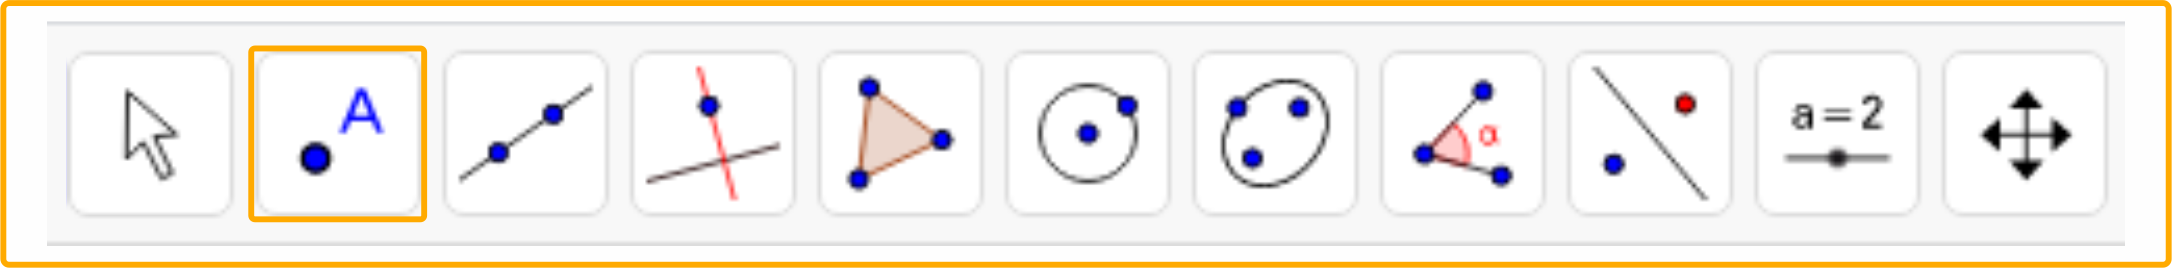
\includegraphics[height=1cm]{Figuras/T01_Ferramenta01.png}
    \caption{Destaque para o ícone {\bf Ponto}}
    \label{ponto}
\end{figure}
\begin{figure}[H]
    \centering
    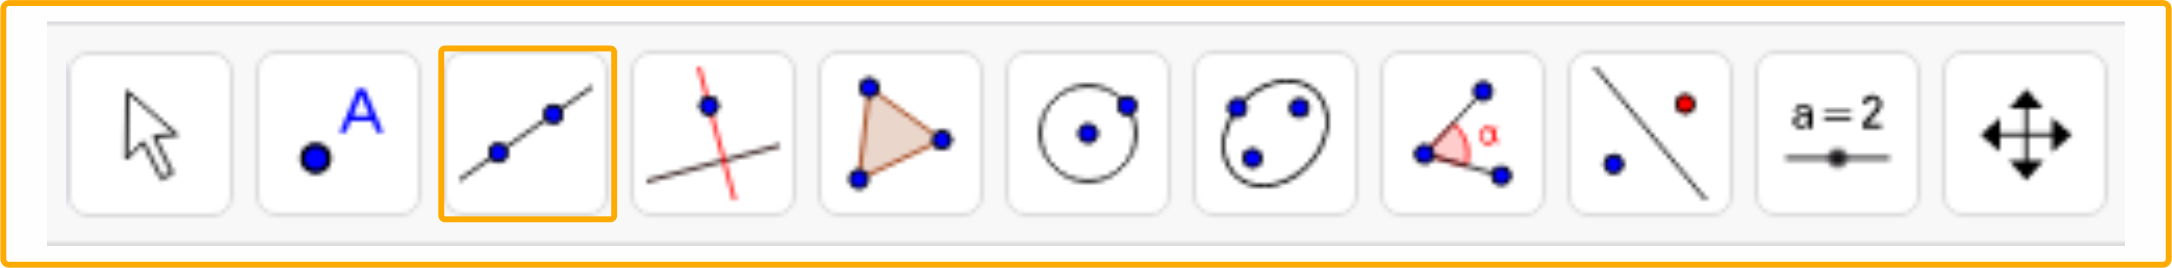
\includegraphics[height=1cm]{Figuras/T01_Ferramenta02.png}
    \caption{Destaque para o ícone {\bf Reta}}
    \label{reta}
\end{figure}
\begin{figure}[H]
    \centering
    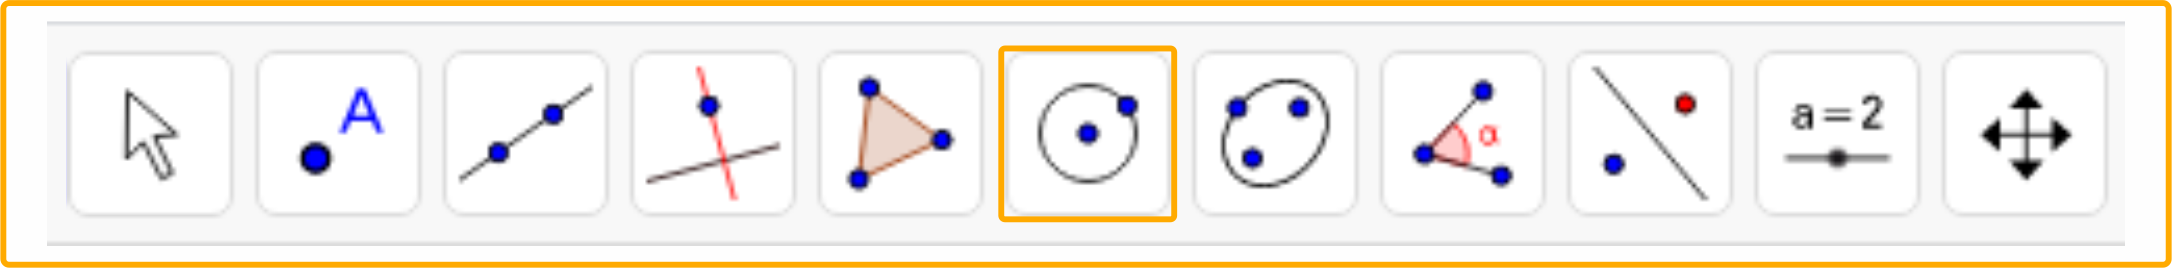
\includegraphics[height=1cm]{Figuras/T01_Ferramenta03.png}
    \caption{Destaque para o ícone {\bf Circunferência}}
    \label{circunferencia}
\end{figure}
\begin{figure}[H]
    \centering
    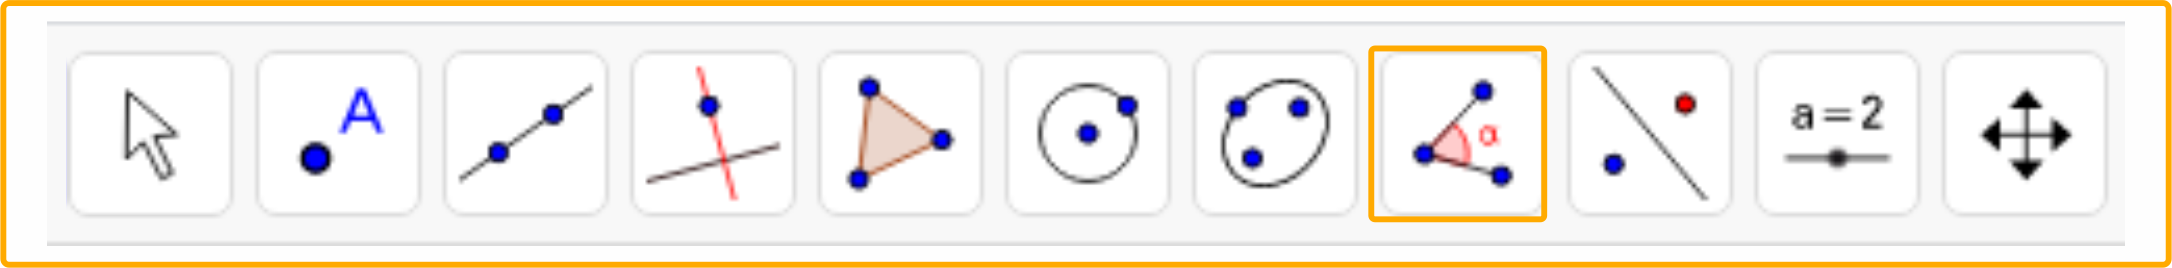
\includegraphics[height=1cm]{Figuras/T01_Ferramenta04.png}
    \caption{Destaque para o ícone {\bf Ângulo}}
    \label{angulo}
\end{figure}

\newpage
%%%%%%% SEÇÃO 03 - USANDO O GEOGEBRA %%%%%%%%
\section{Utilizando o GeoGebra}
O GeoGebra (aglutinação das palavras Geometria e Álgebra) é um aplicativo matemático que permite realizar construções geométricas, além de inserir funções, equações e coordenadas e alterar todos esses objetos dinamicamente. O melhor de tudo: é um programa gratuito e disponível em várias línguas, entre elas o Português.
Você pode fazer o download do GeoGebra acessando sua página \href{https://www.geogebra.org/}{{\color{blue}{clicando aqui}}}

%%%%%%% SUBSEÇÃO 01 - ATIVIDADE 01 %%%%%%%%
\subsection{Atividade I: Determinação do ponto médio de um segmento de reta}

\begin{enumerate}[{Etapa} 1.]
\item Selecione o ícone em destaque e clique na opção {\it reta}\label{Atividade01_Etapa01}

\begin{figure}[H]
    \centering
    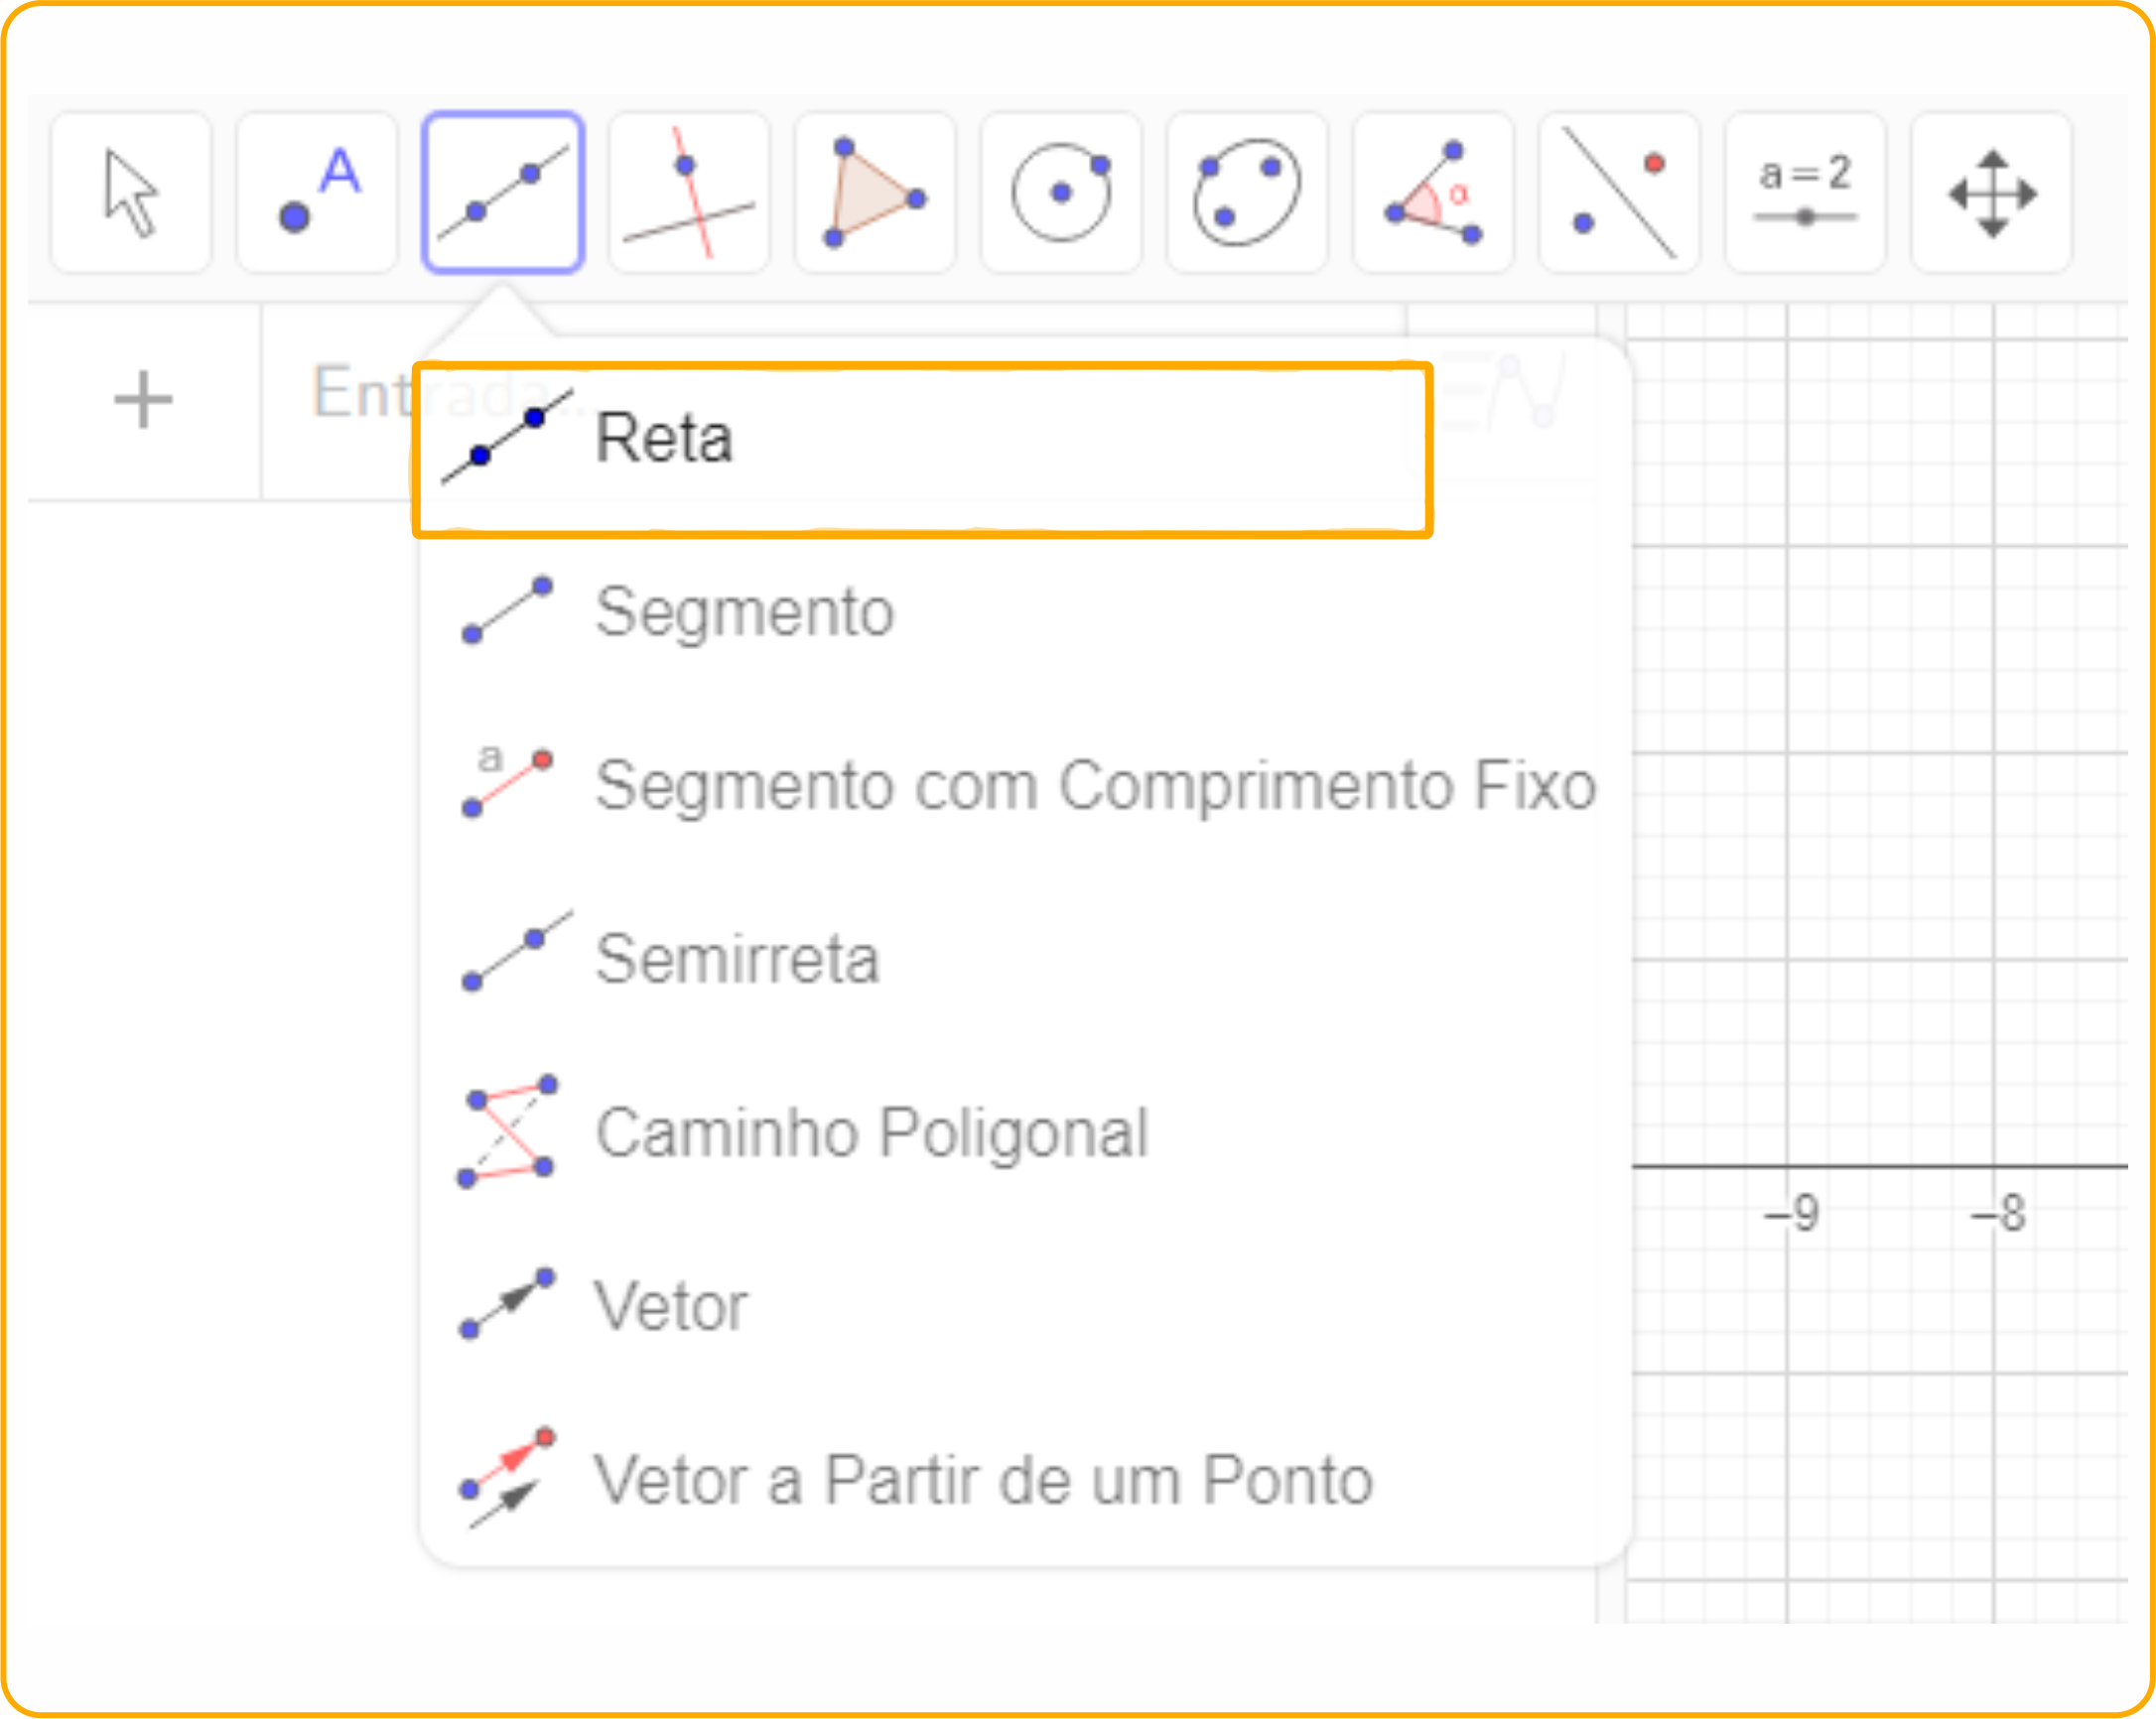
\includegraphics[height=8cm]{Figuras/T01_Elemento02.png}
    \caption{Atividade I - Etapa \ref{Atividade01_Etapa01}}
    \label{Atividade01_Etapa01_Imagem}
\end{figure}

\item Construa a reta $r$ que passe pelos pontos $A$ e $B$, sendo a coordenada do ponto $A (0,0)$ e do ponto $B (4,0)$. \label{Atividade01_Etapa02}

\begin{figure}[H]
    \centering
    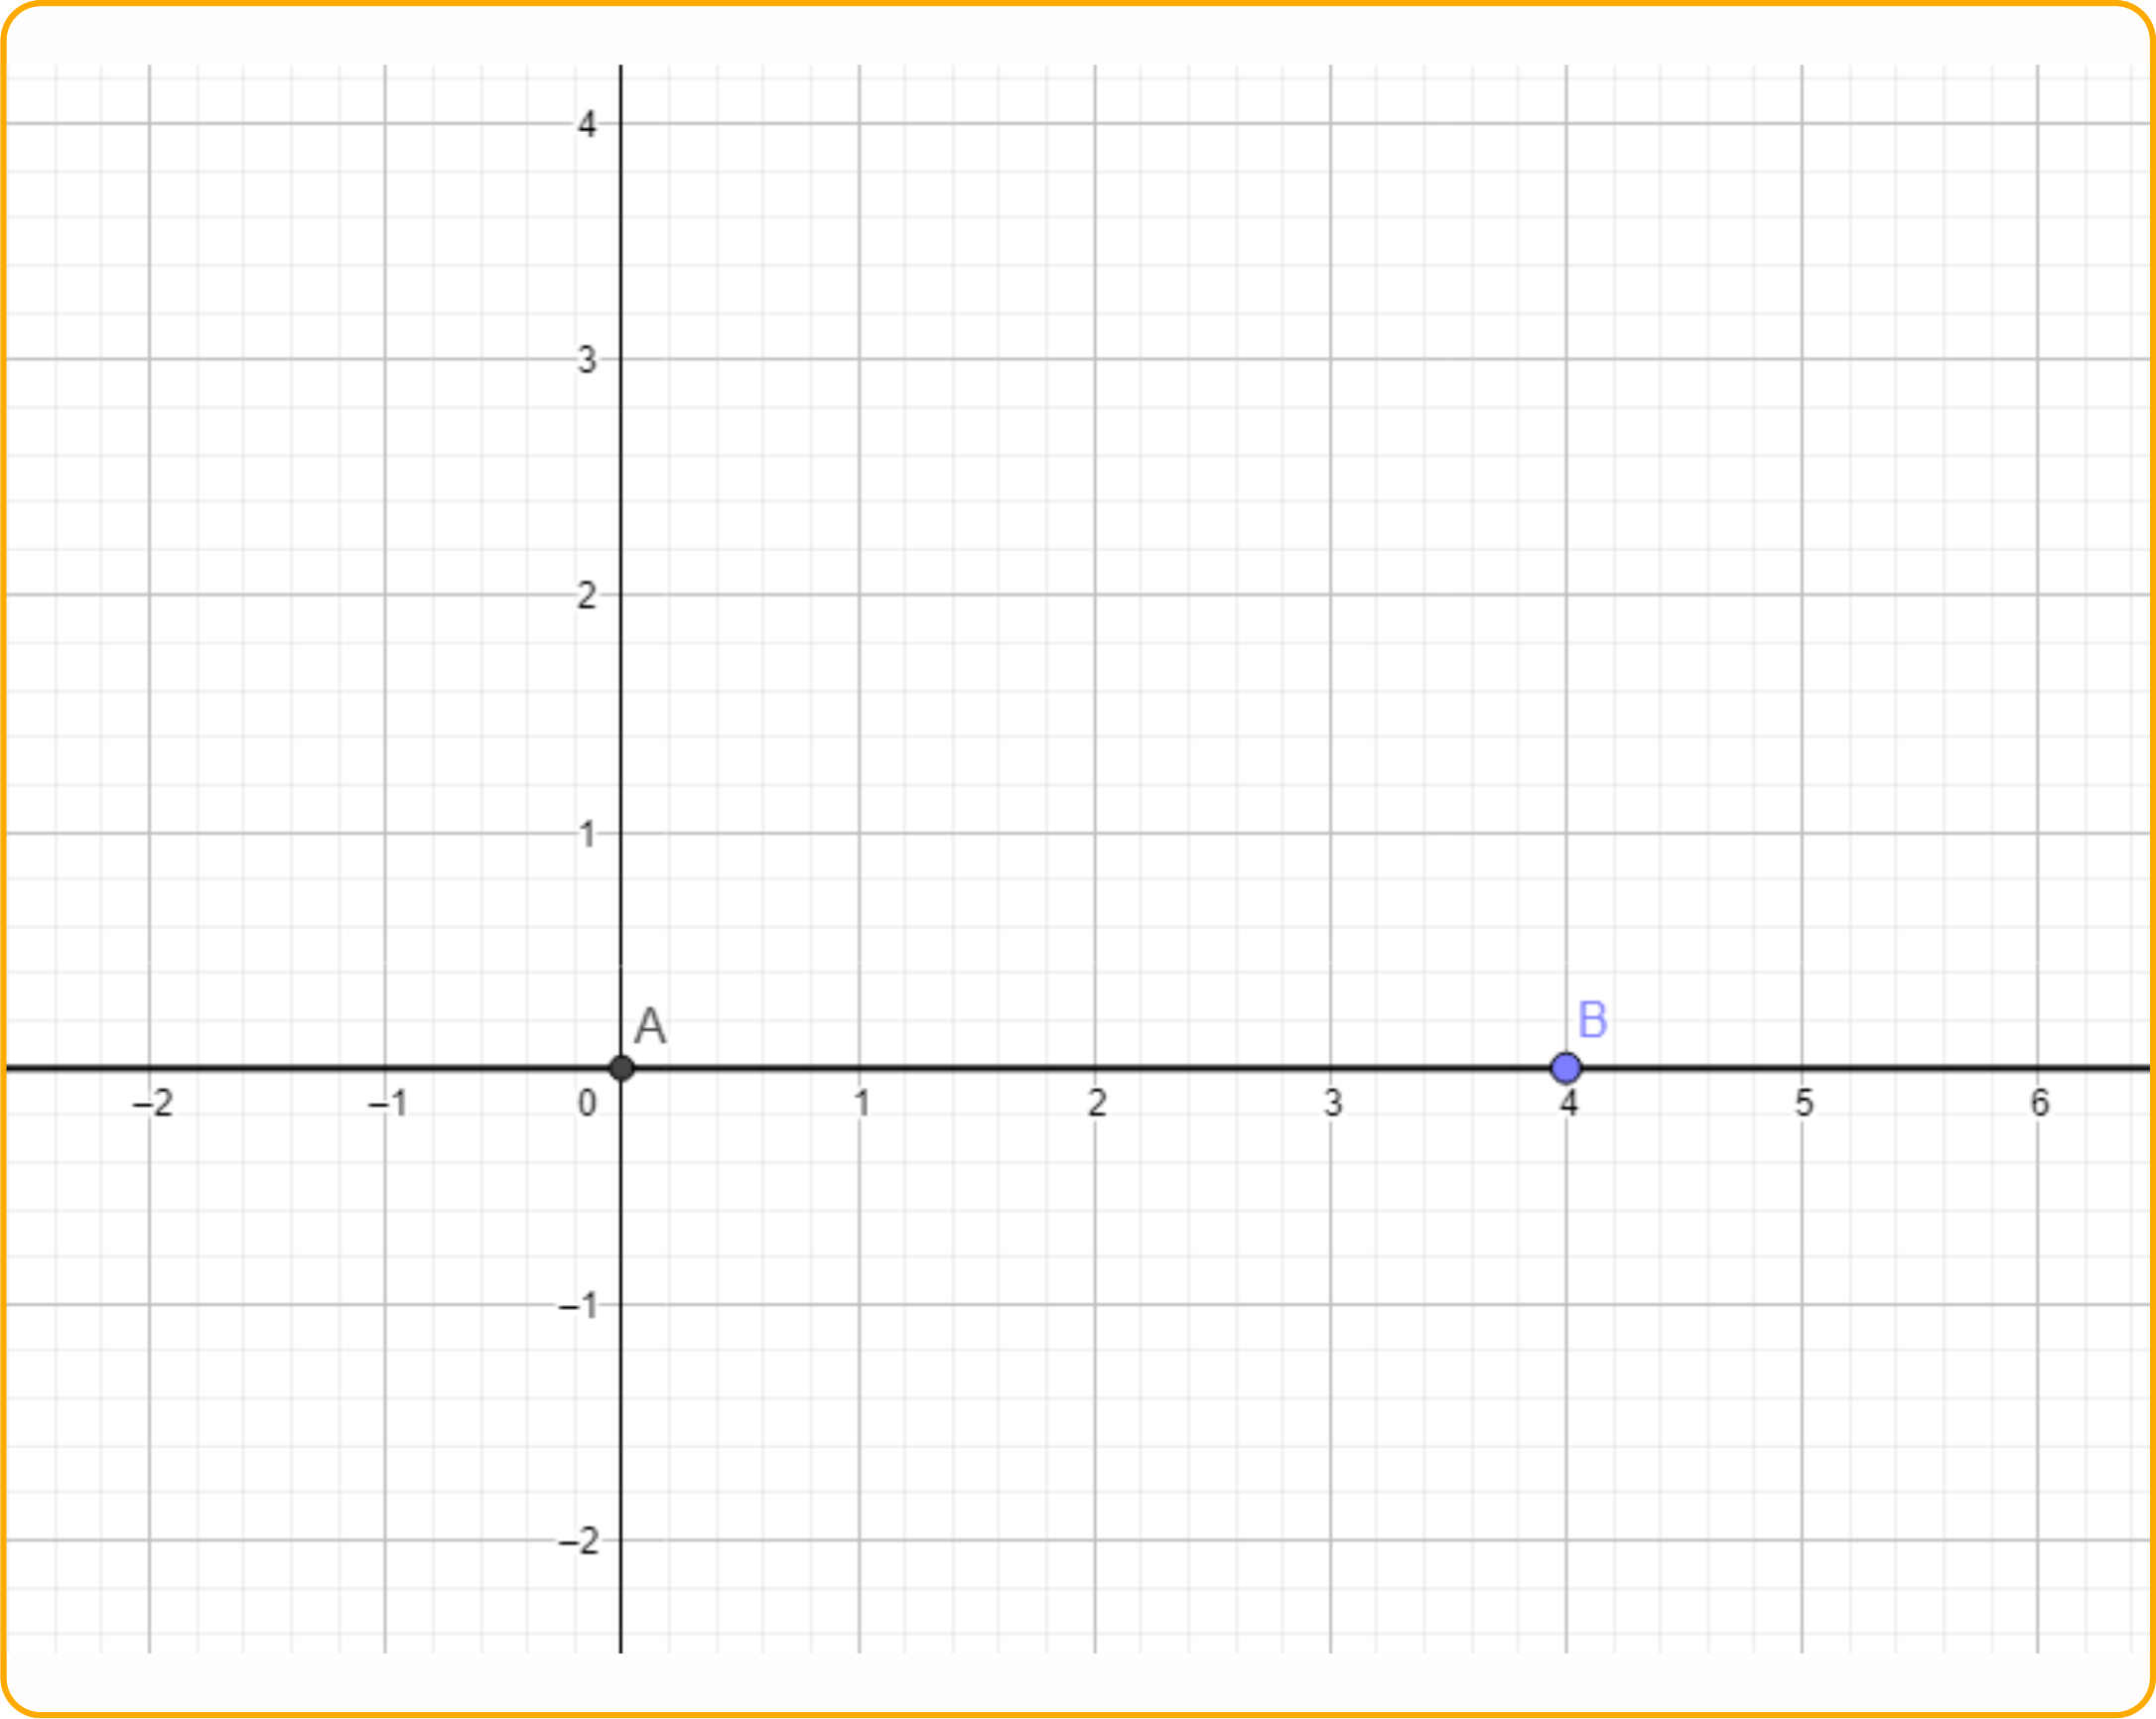
\includegraphics[height=8cm]{Figuras/T01_Atividade01_Fig01.png}
\caption{Atividade I - Etapa \ref{Atividade01_Etapa02}}
    \label{Atividade01_Etapa02_Imagem}
\end{figure}

\item Selecione o ícone em destaque e clique na opção {\it compasso} \label{Atividade01_Etapa03}

\begin{figure}[H]
    \centering
    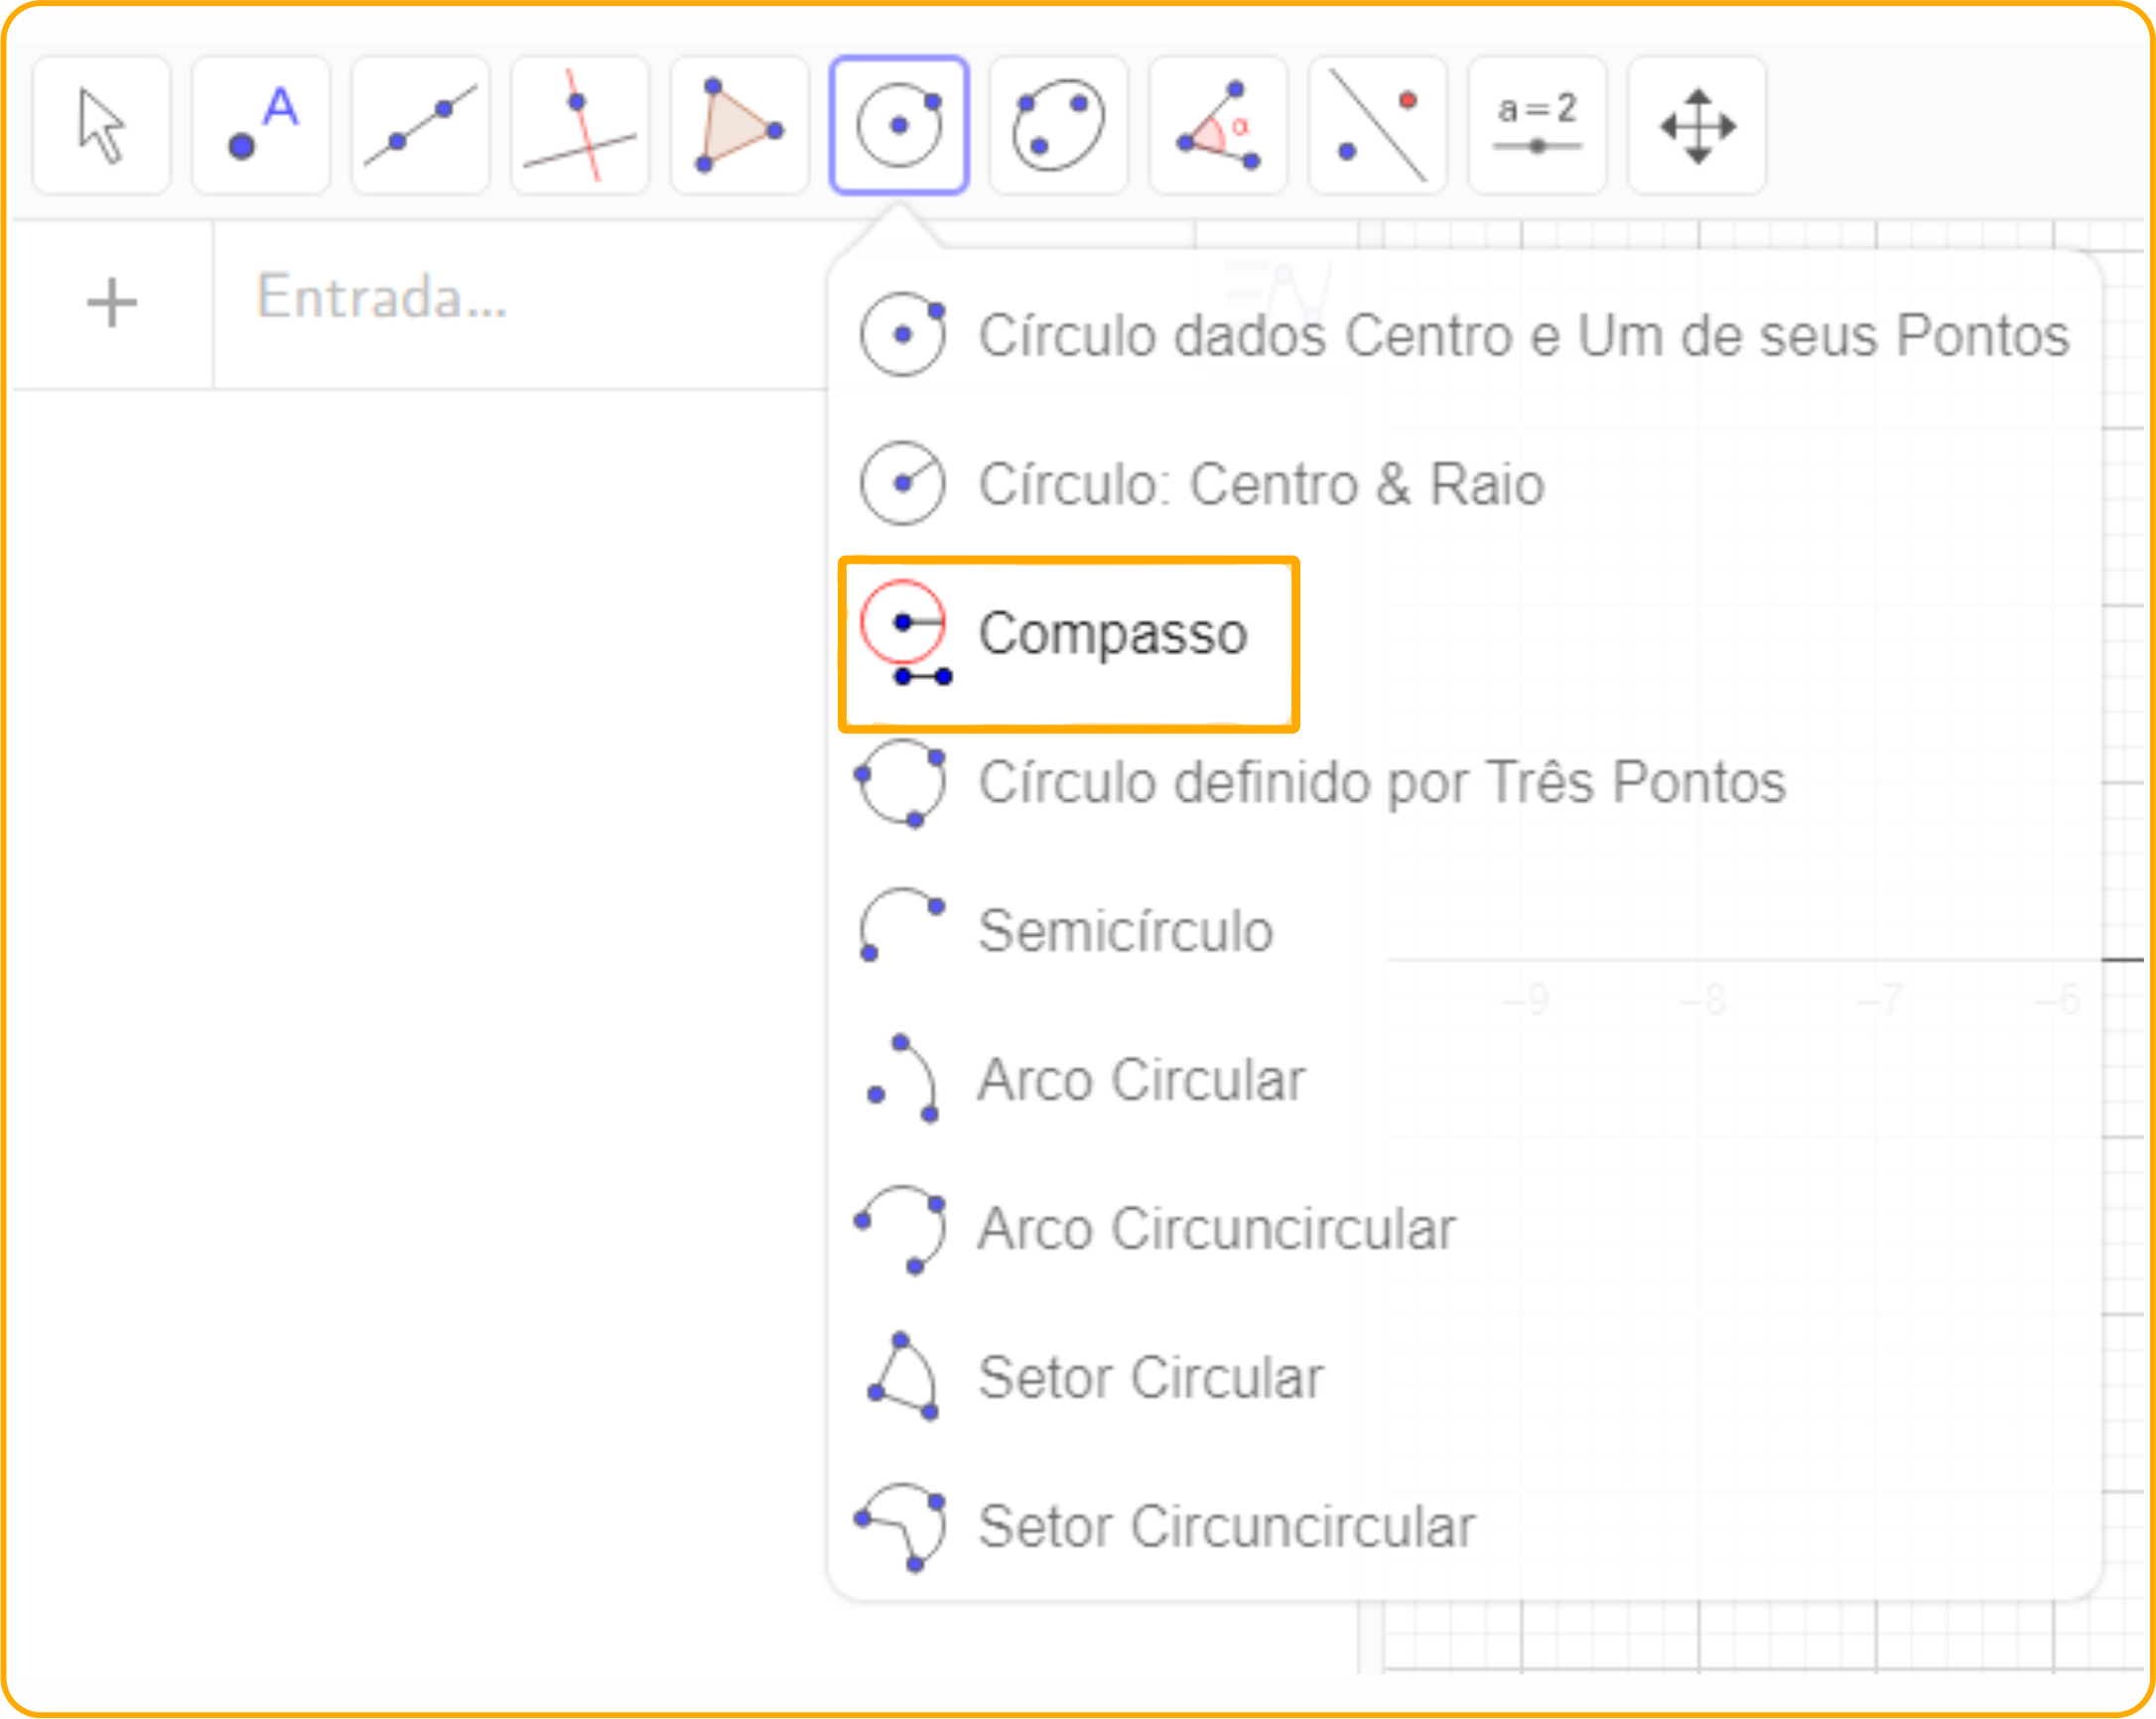
\includegraphics[height=8cm]{Figuras/T01_Elemento04.png}
    \caption{Atividade I - Etapa \ref{Atividade01_Etapa03}}
    \label{Atividade01_Etapa03_Imagem}
\end{figure}

\item Construa uma circunferência $c$ com centro no ponto $A$ e com raio de mesma medida que o segmento $\overline{AB}$ \label{Atividade01_Etapa04}

\begin{figure}[H]
    \centering
    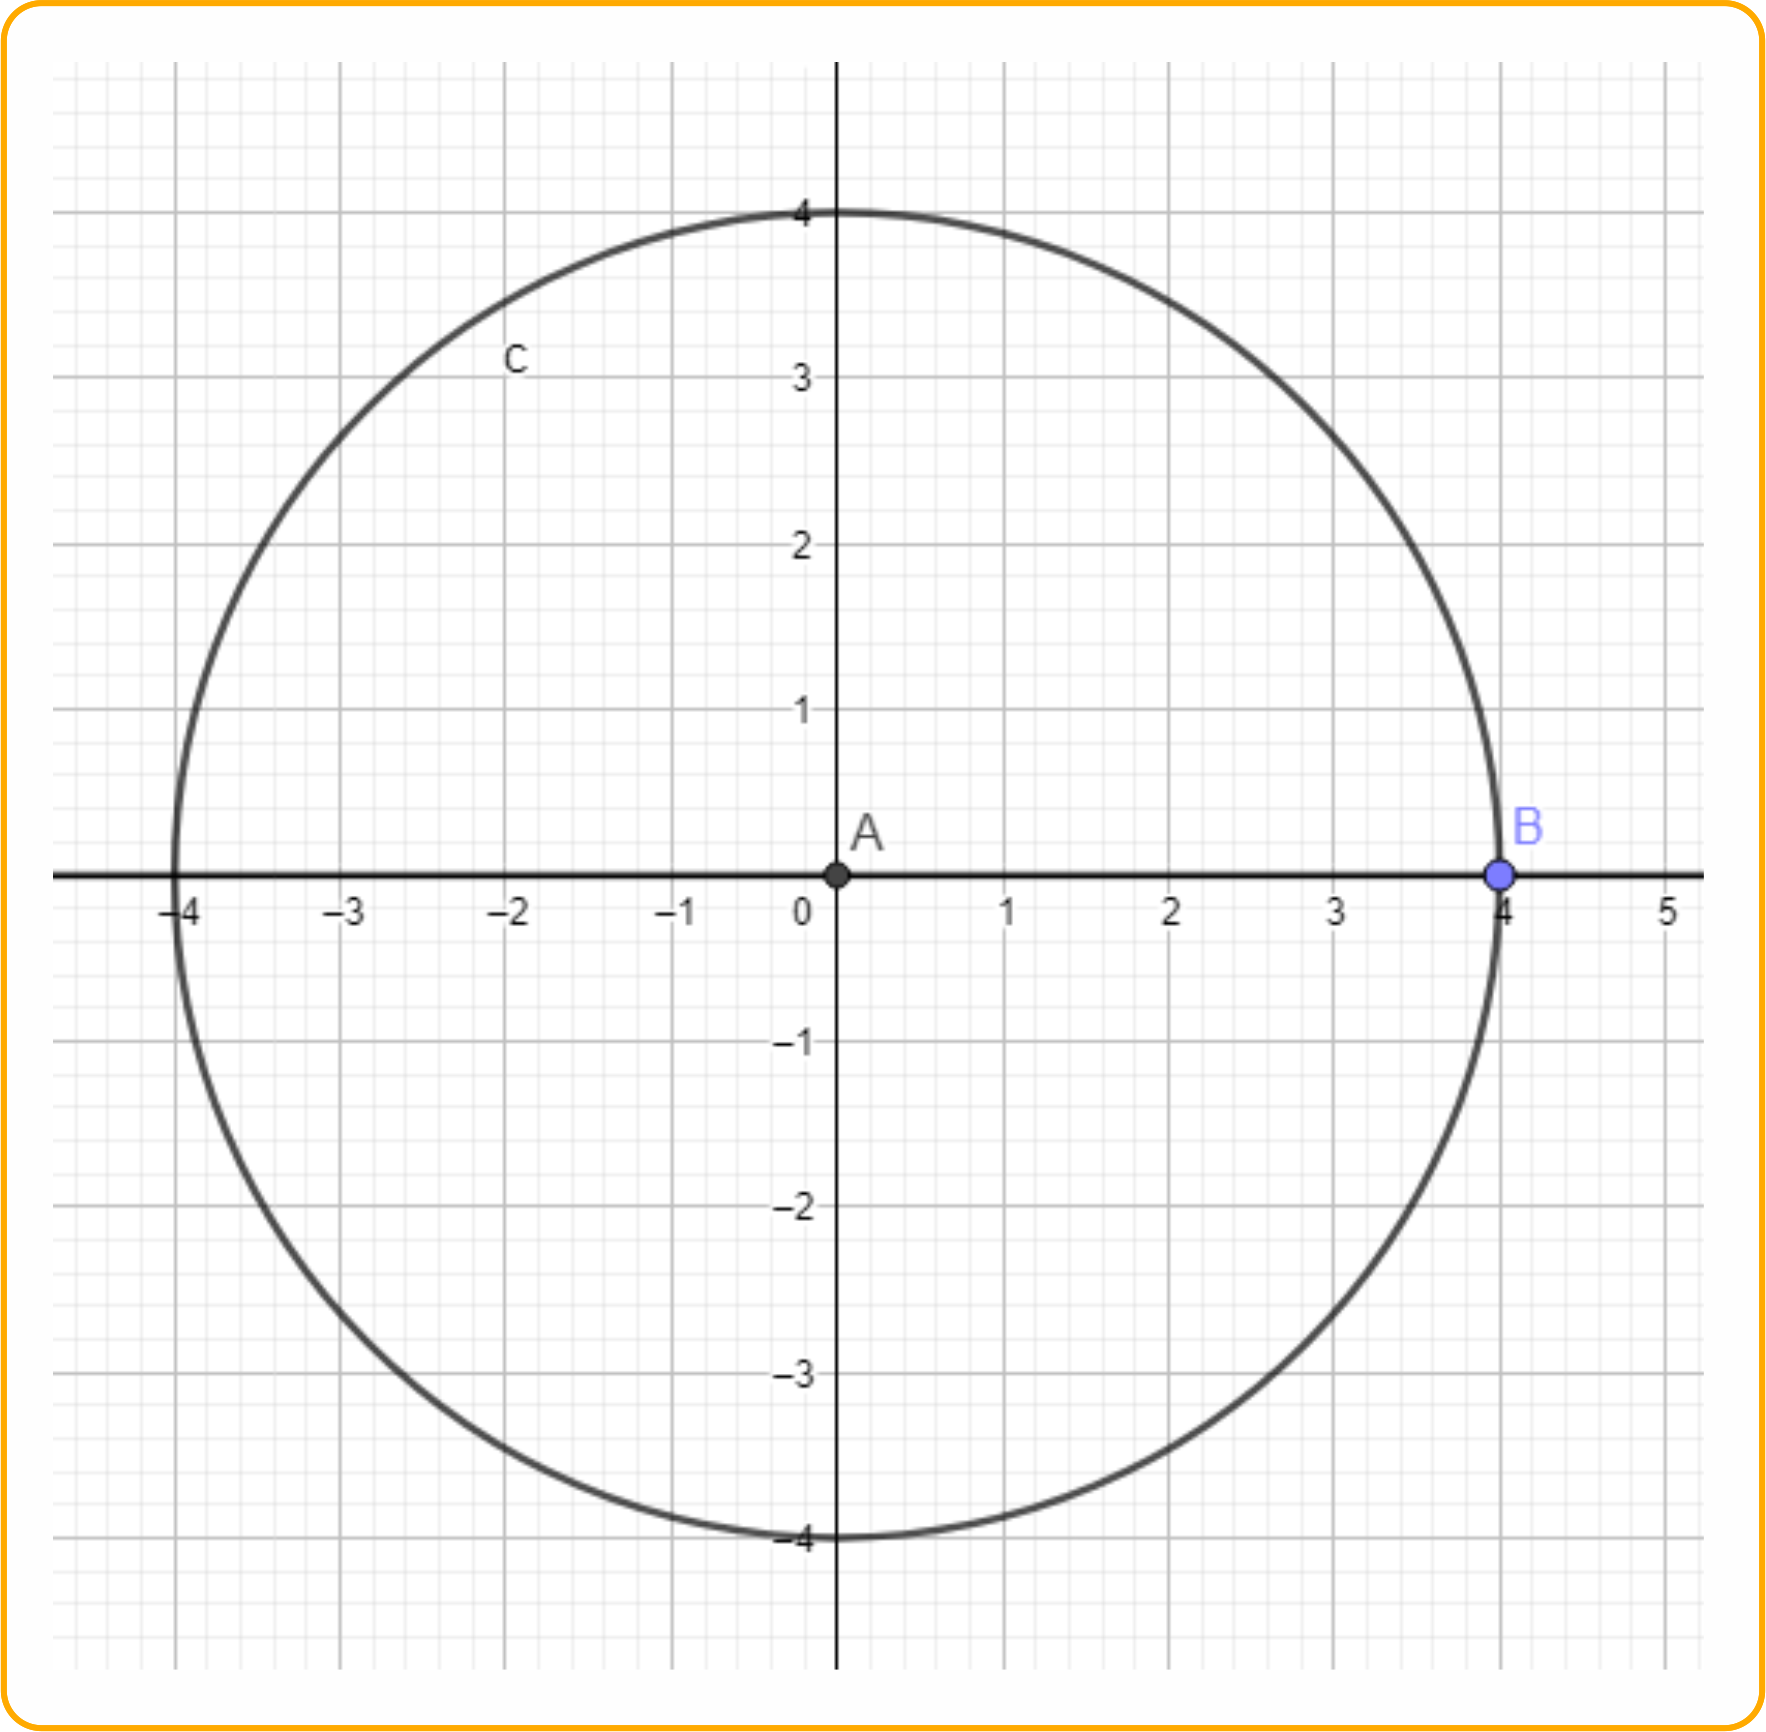
\includegraphics[height=8cm]{Figuras/T01_Atividade01_Fig02.png}
    \caption{Atividade I - Etapa \ref{Atividade01_Etapa04}}
    \label{Atividade01_Etapa04_Imagem}
\end{figure}

\item Construa uma outra circunferência $d$, agora com centro no ponto $B$ e com raio de mesma medida que o segmento $\overline{AB}$ \label{Atividade01_Etapa05}

\begin{figure}[H]
    \centering
    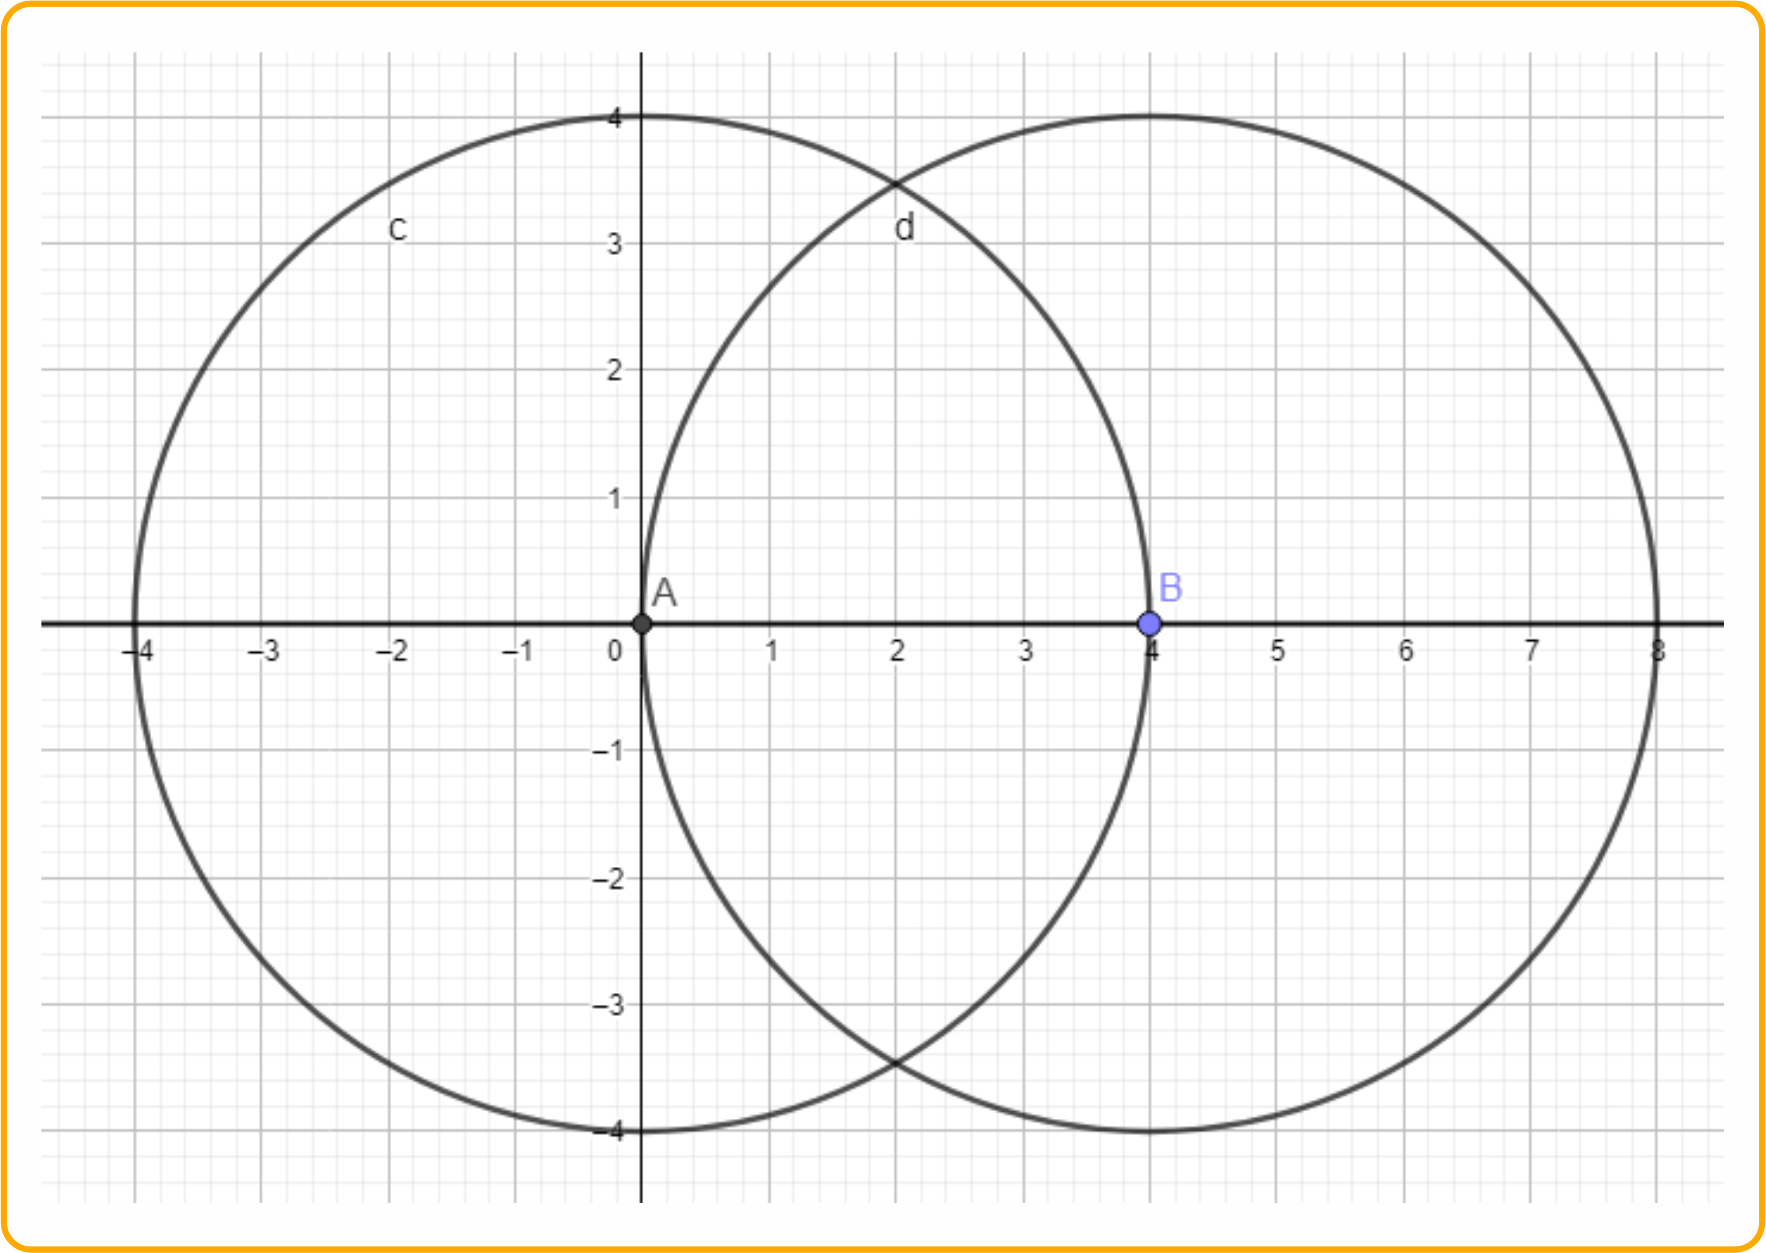
\includegraphics[height=8cm]{Figuras/T01_Atividade01_Fig03.png}
    \caption{Atividade I - Etapa \ref{Atividade01_Etapa05}}
    \label{Atividade01_Etapa05_Imagem}
\end{figure}

\item Selecione o ícone em destaque e clique na opção {\it interseção de dois objetos} \label{Atividade01_Etapa06}
\begin{figure}[H]
    \centering
    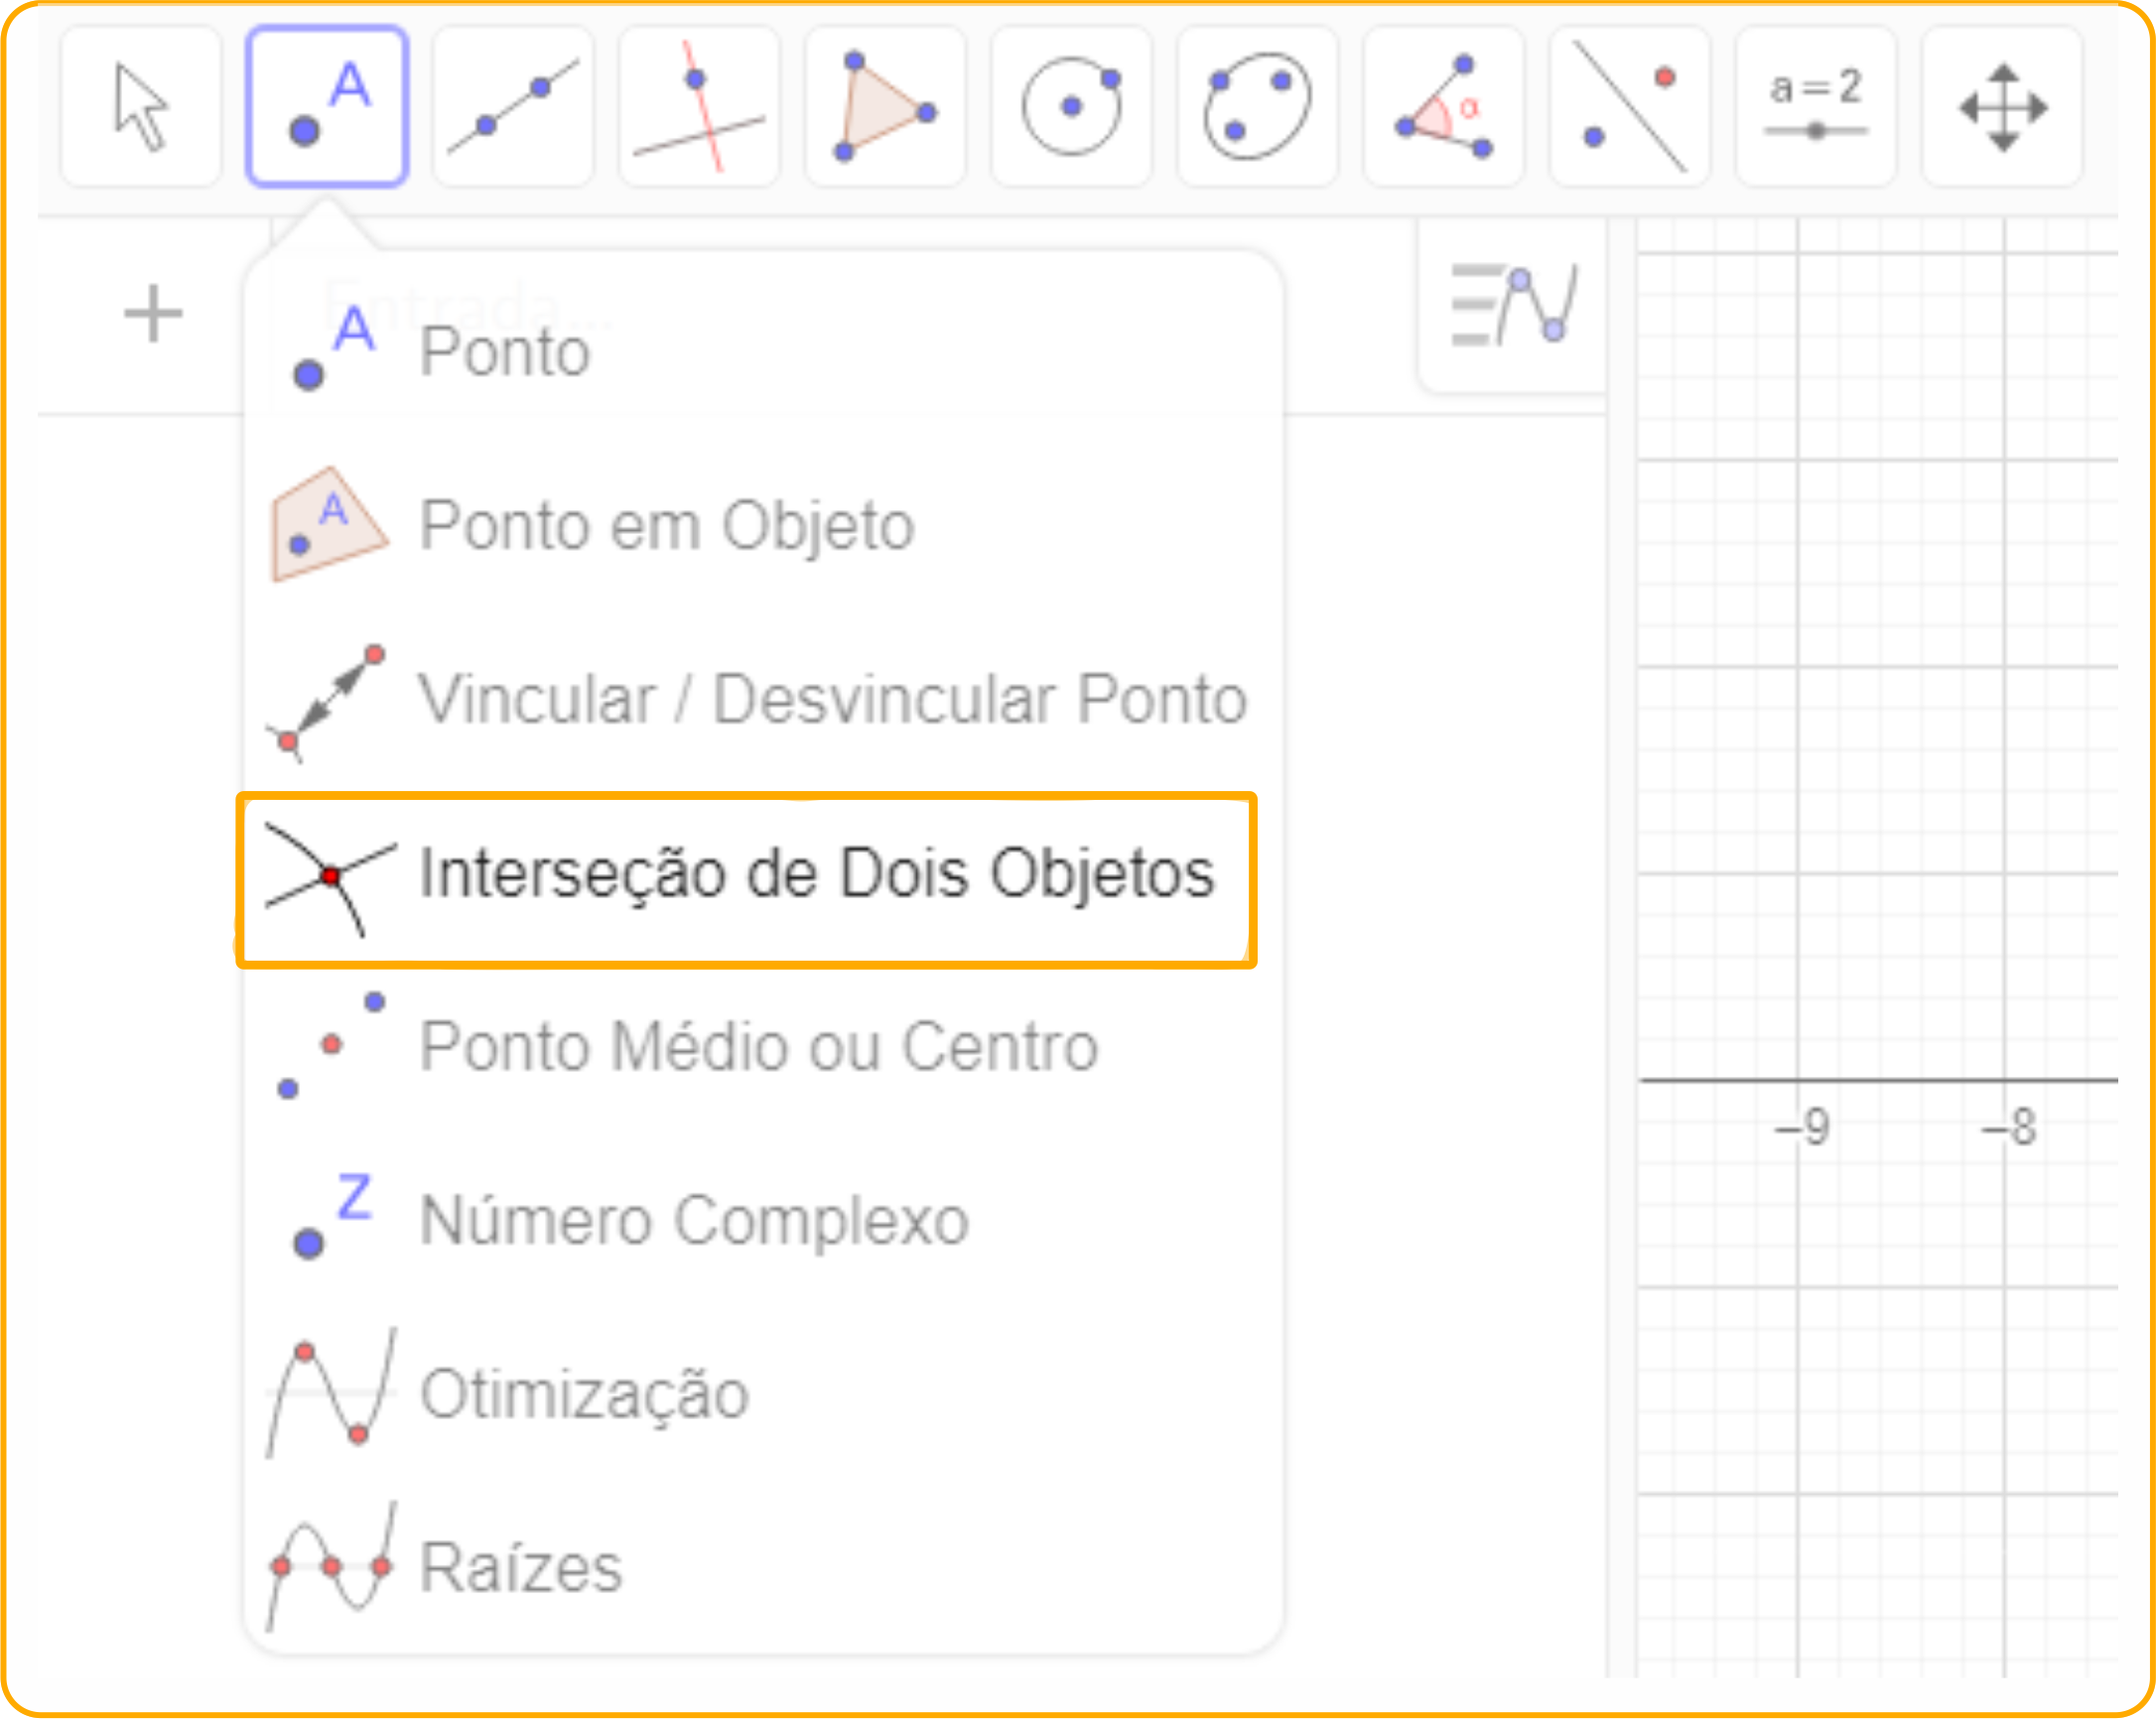
\includegraphics[height=8cm]{Figuras/T01_Elemento05.png}
    \caption{Atividade I - Etapa \ref{Atividade01_Etapa06}}
    \label{Atividade01_Etapa06_Imagem}
\end{figure}

\item Marque os pontos $C$ e $D$ nas interseções entre as circunferências $c$ e $d$ \label{Atividade01_Etapa07}

\begin{figure}[H]
    \centering
    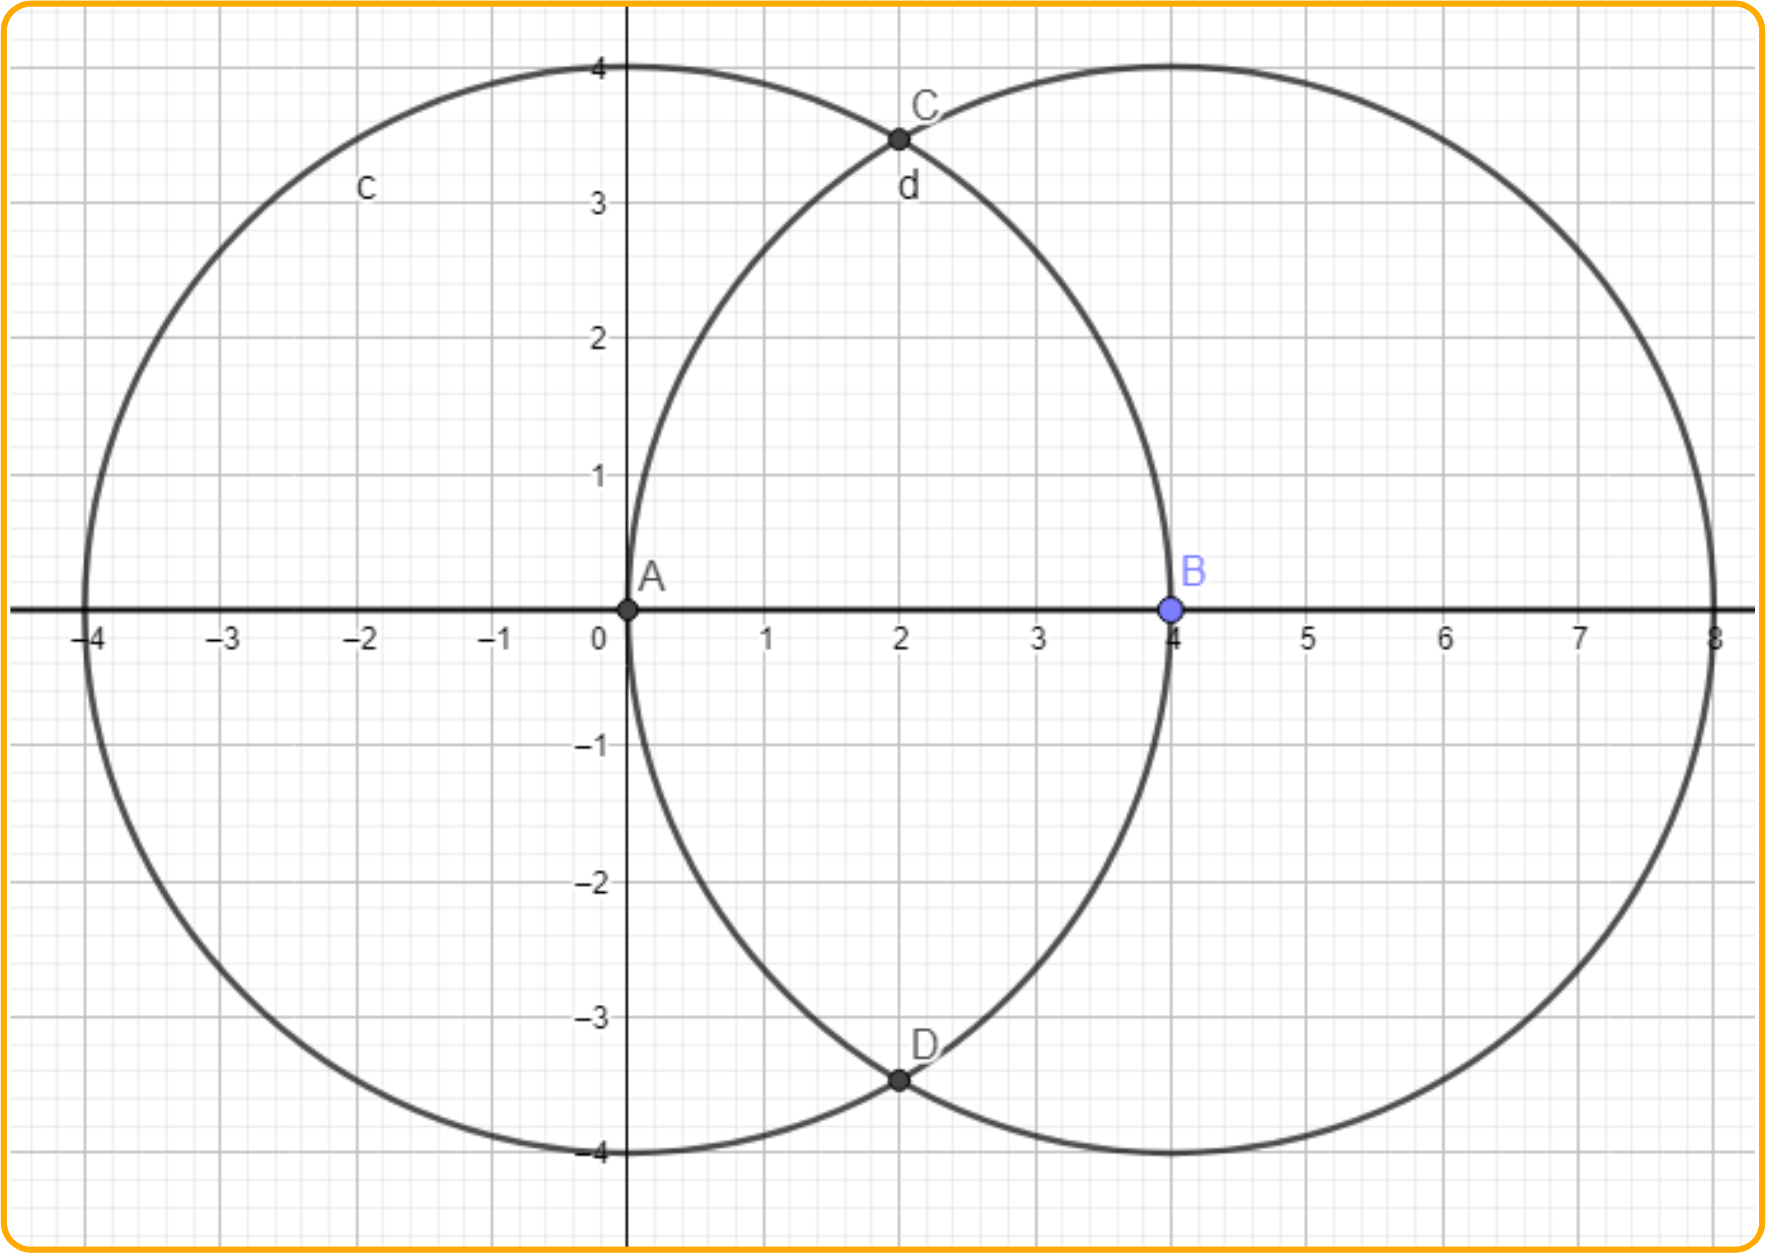
\includegraphics[height=8cm]{Figuras/T01_Atividade01_Fig04.png}
    \caption{Atividade I - Etapa \ref{Atividade01_Etapa07}}
    \label{Atividade01_Etapa07_Imagem}
\end{figure}

\item Selecione o ícone em destaque e clique na opção {\it segmento} \label{Atividade01_Etapa08}
\begin{figure}[H]
    \centering
    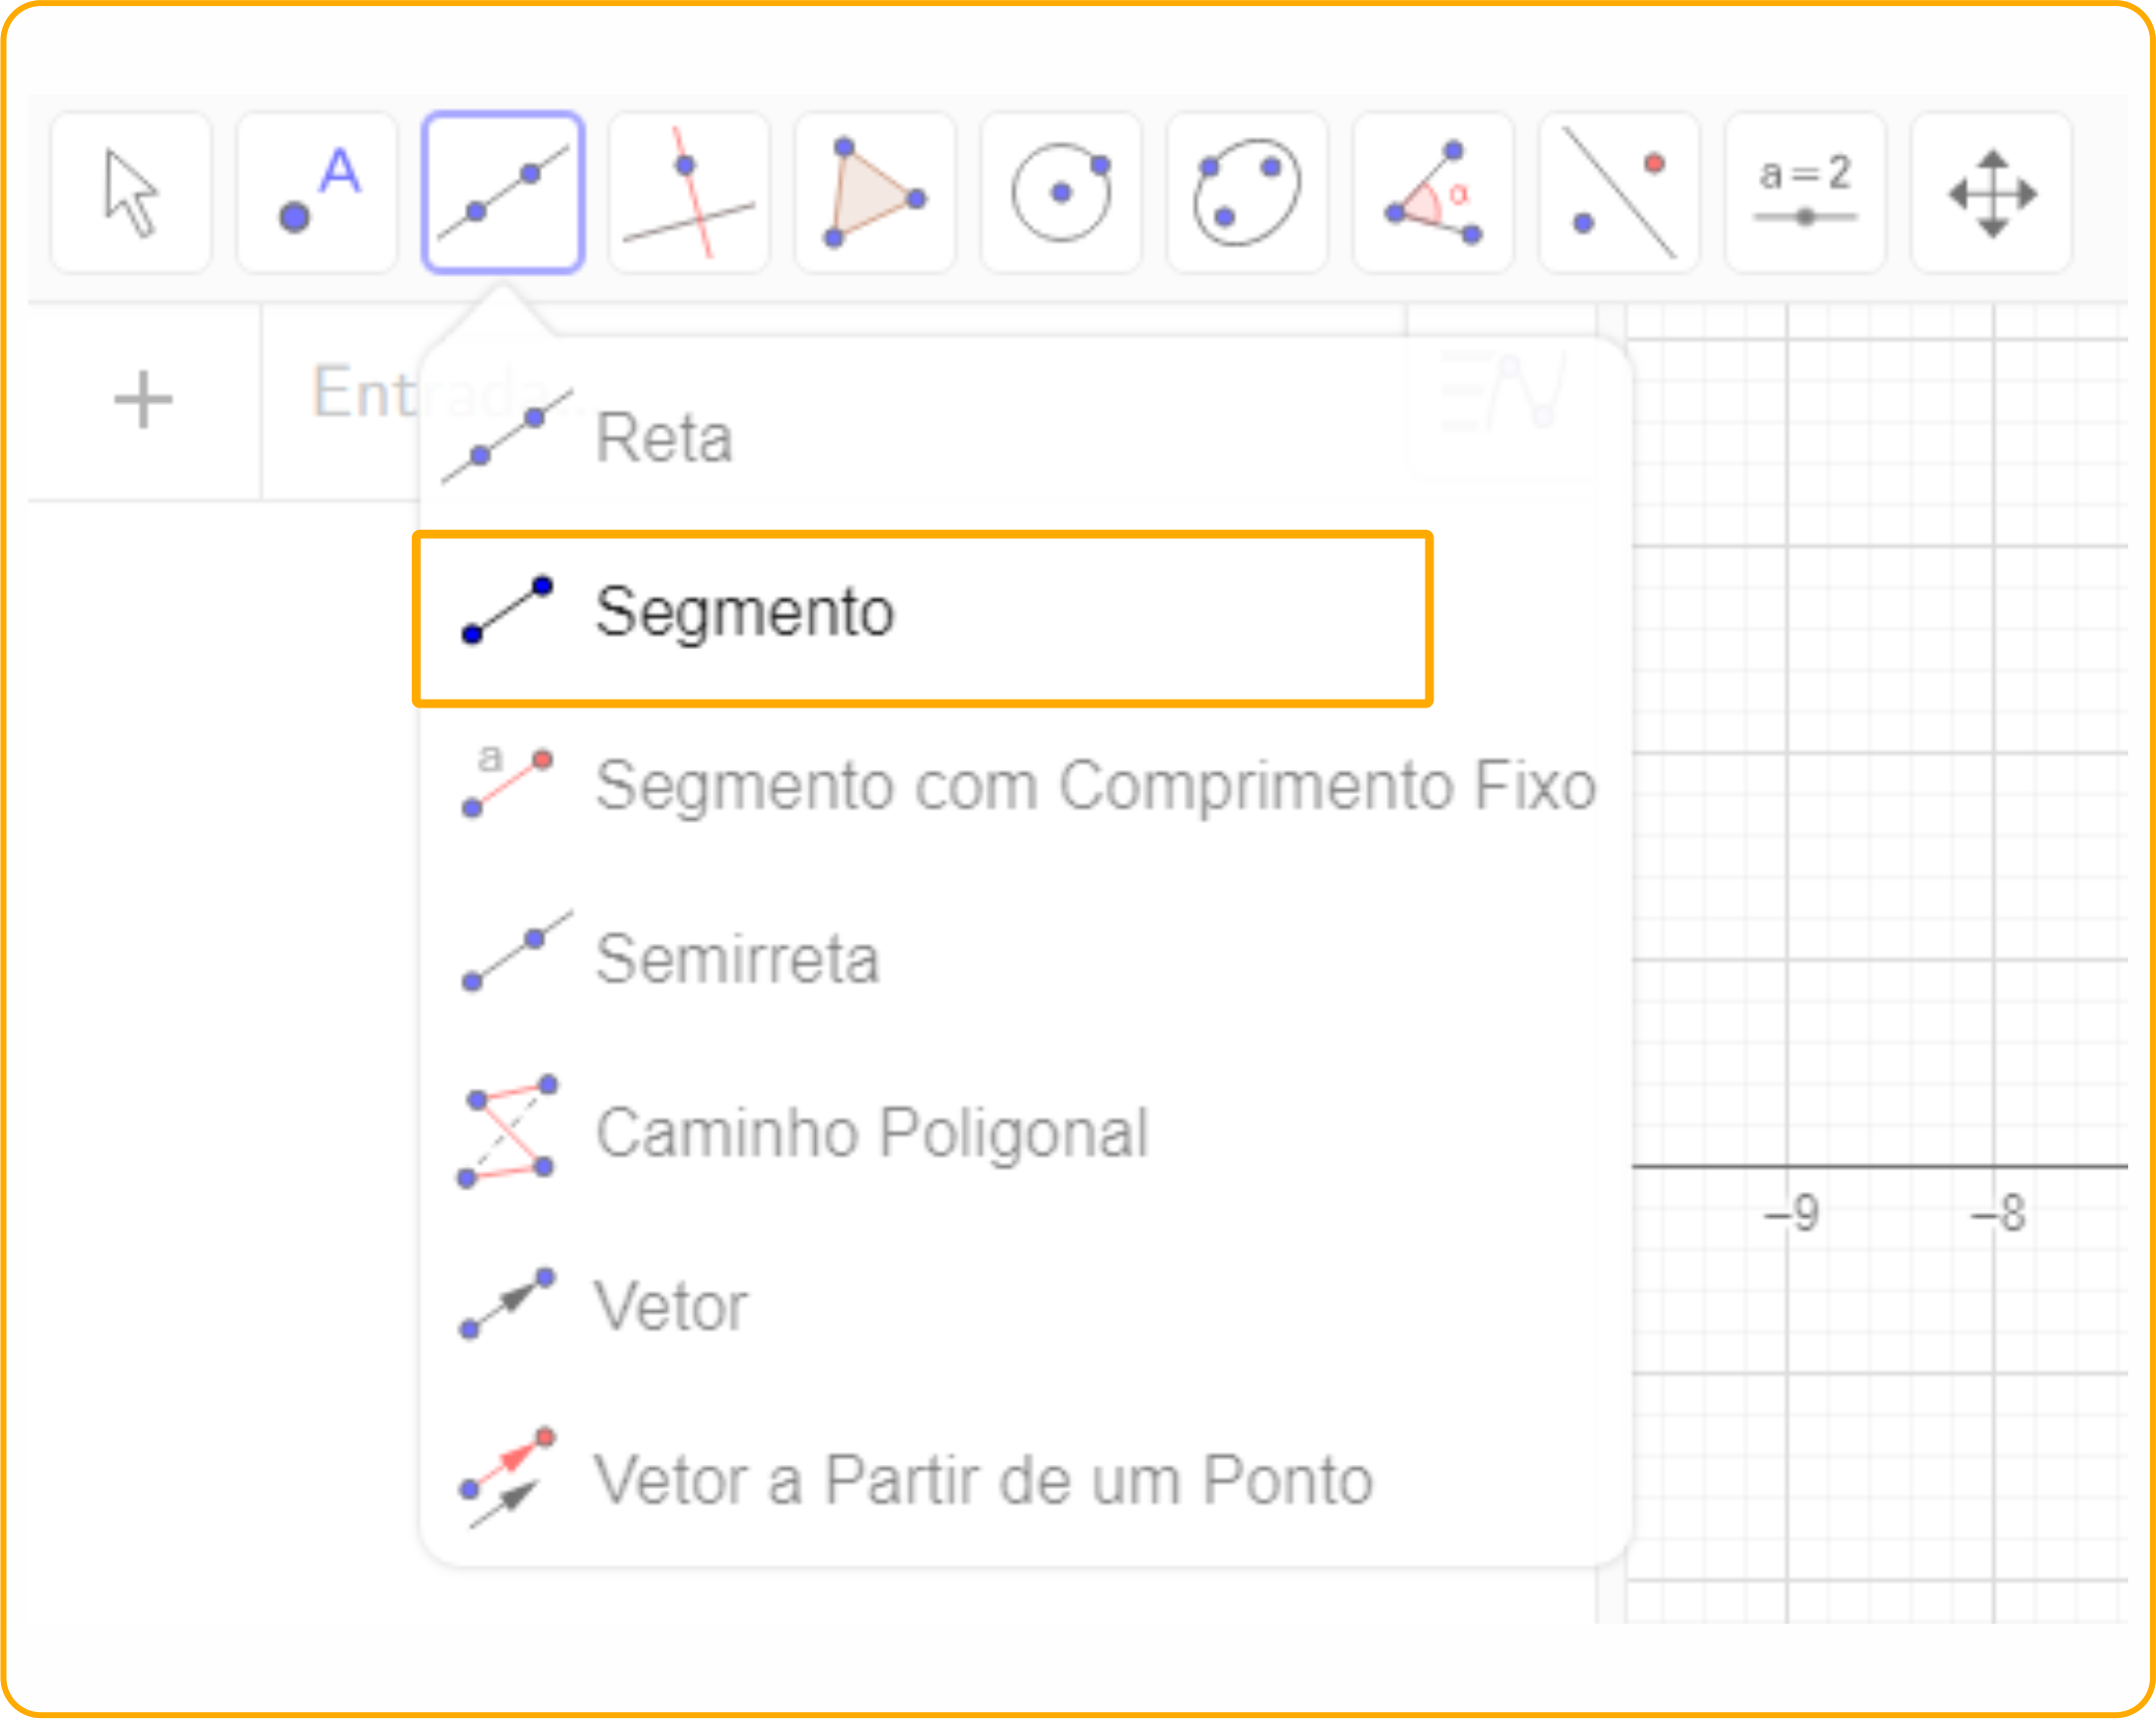
\includegraphics[height=8cm]{Figuras/T01_Elemento06.png}
    \caption{Atividade I - Etapa \ref{Atividade01_Etapa08}}
    \label{Atividade01_Etapa08_Imagem}
\end{figure}

\item Construa o segmento de reta $\overline{CD}$ \label{Atividade01_Etapa09}
\begin{figure}[H]
    \centering
    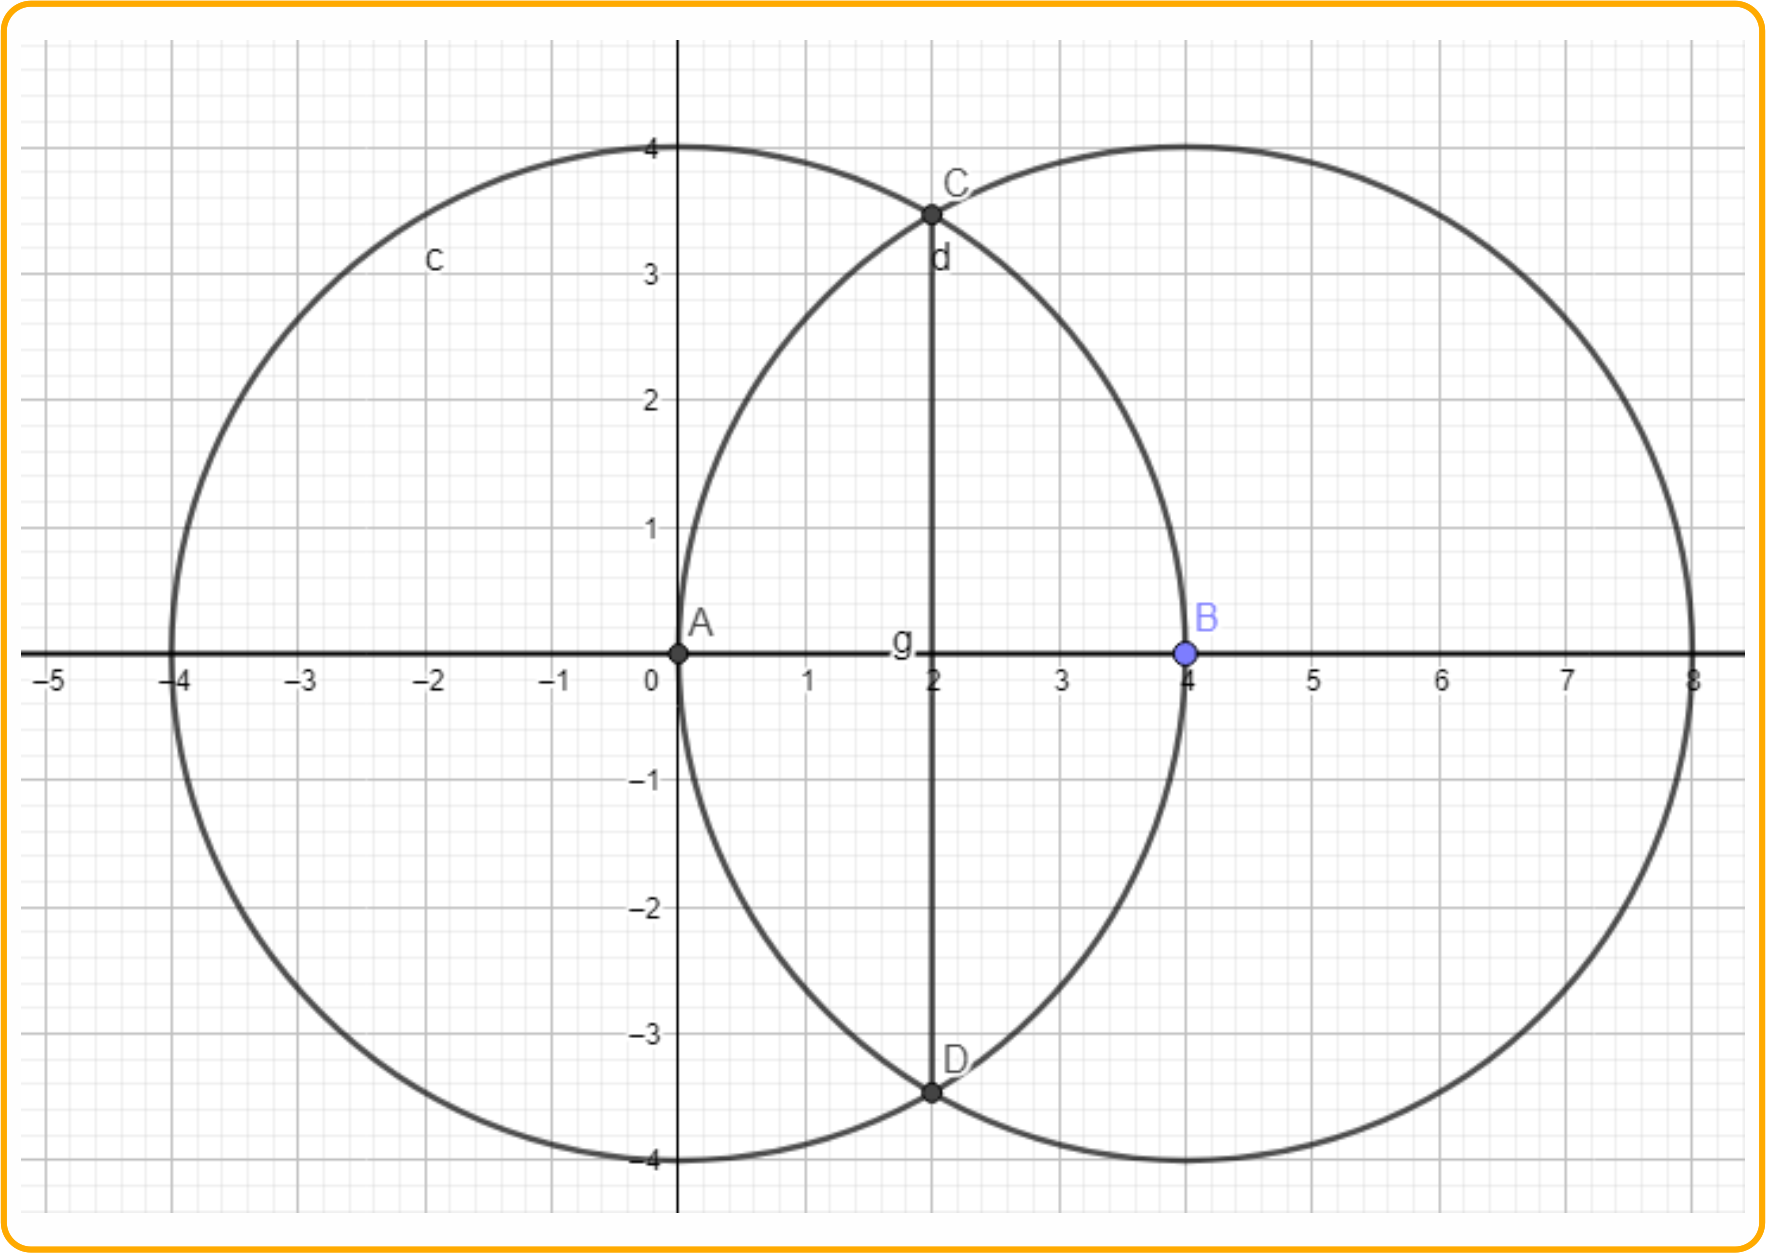
\includegraphics[height=8cm]{Figuras/T01_Atividade01_Fig05.png}
    \caption{Atividade I - Etapa \ref{Atividade01_Etapa09}}
    \label{Atividade01_Etapa09_Imagem}
\end{figure}

\item Repita a Etapa \ref{Atividade01_Etapa06} e marque o ponto $E$ na interseção entre o segmento $\overline{CD}$ e a reta $r$. Note que a coordenada do ponto $E$, indicado na barra lateral do GeoGebra, é $(2,0)$, pois trata-se do ponto médio do segmento $\overline{AB}$! \label{Atividade01_Etapa10}

\begin{figure}[H]
    \centering
    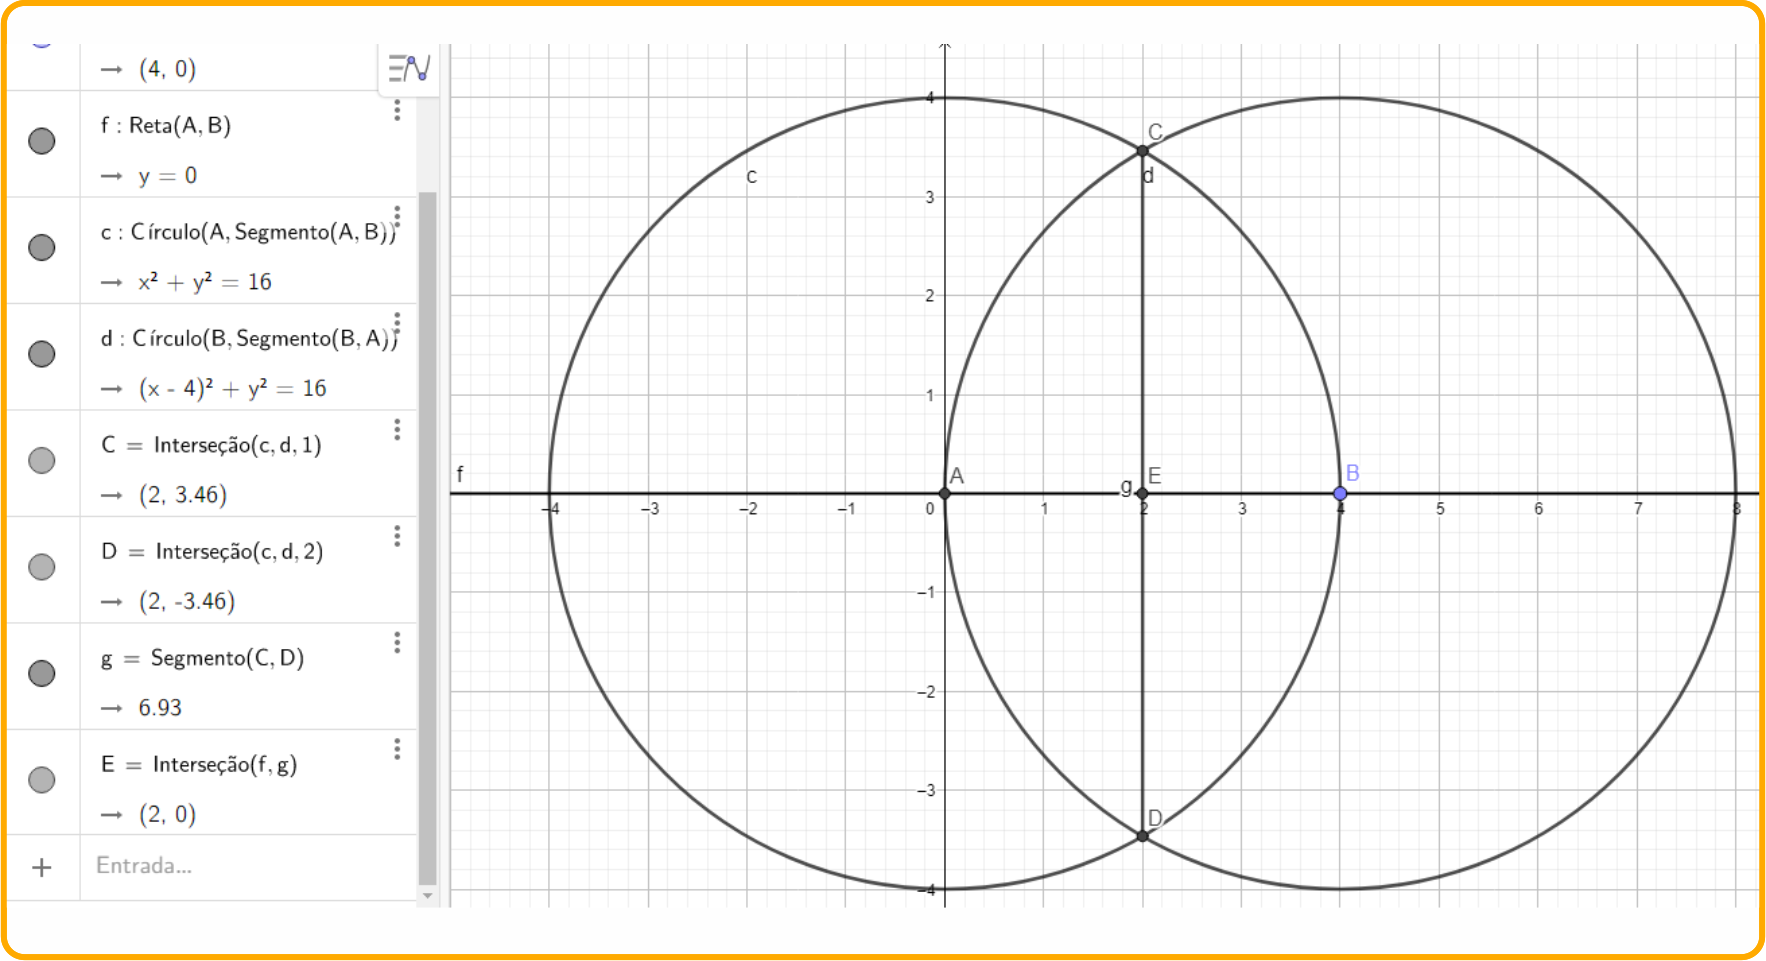
\includegraphics[height=8cm]{Figuras/T01_Atividade01_Fig06.png}
    \caption{Atividade I - Etapa \ref{Atividade01_Etapa10}}
    \label{Atividade01_Etapa10_Imagem}
\end{figure}
\end{enumerate}
O segmento $\overline{CD}$ é a mediatriz do segmento $\overline{AB}$, uma vez que por construção, ABCD forma um losango e, assim, suas diagonais são perpendiculares e cortam-se ao meio (no ponto $E$).

\newpage

%%%%%%% SUBSEÇÃO 02 - ATIVIDADE 02 %%%%%%%%
\subsection{Atividade II: Construção de retas paralelas}

\begin{enumerate}[{Etapa} 1.] 
\item Selecione o ícone em destaque e clique na opção {\it reta} \label{Atividade02_Etapa01}
\begin{figure}[H]
    \centering
    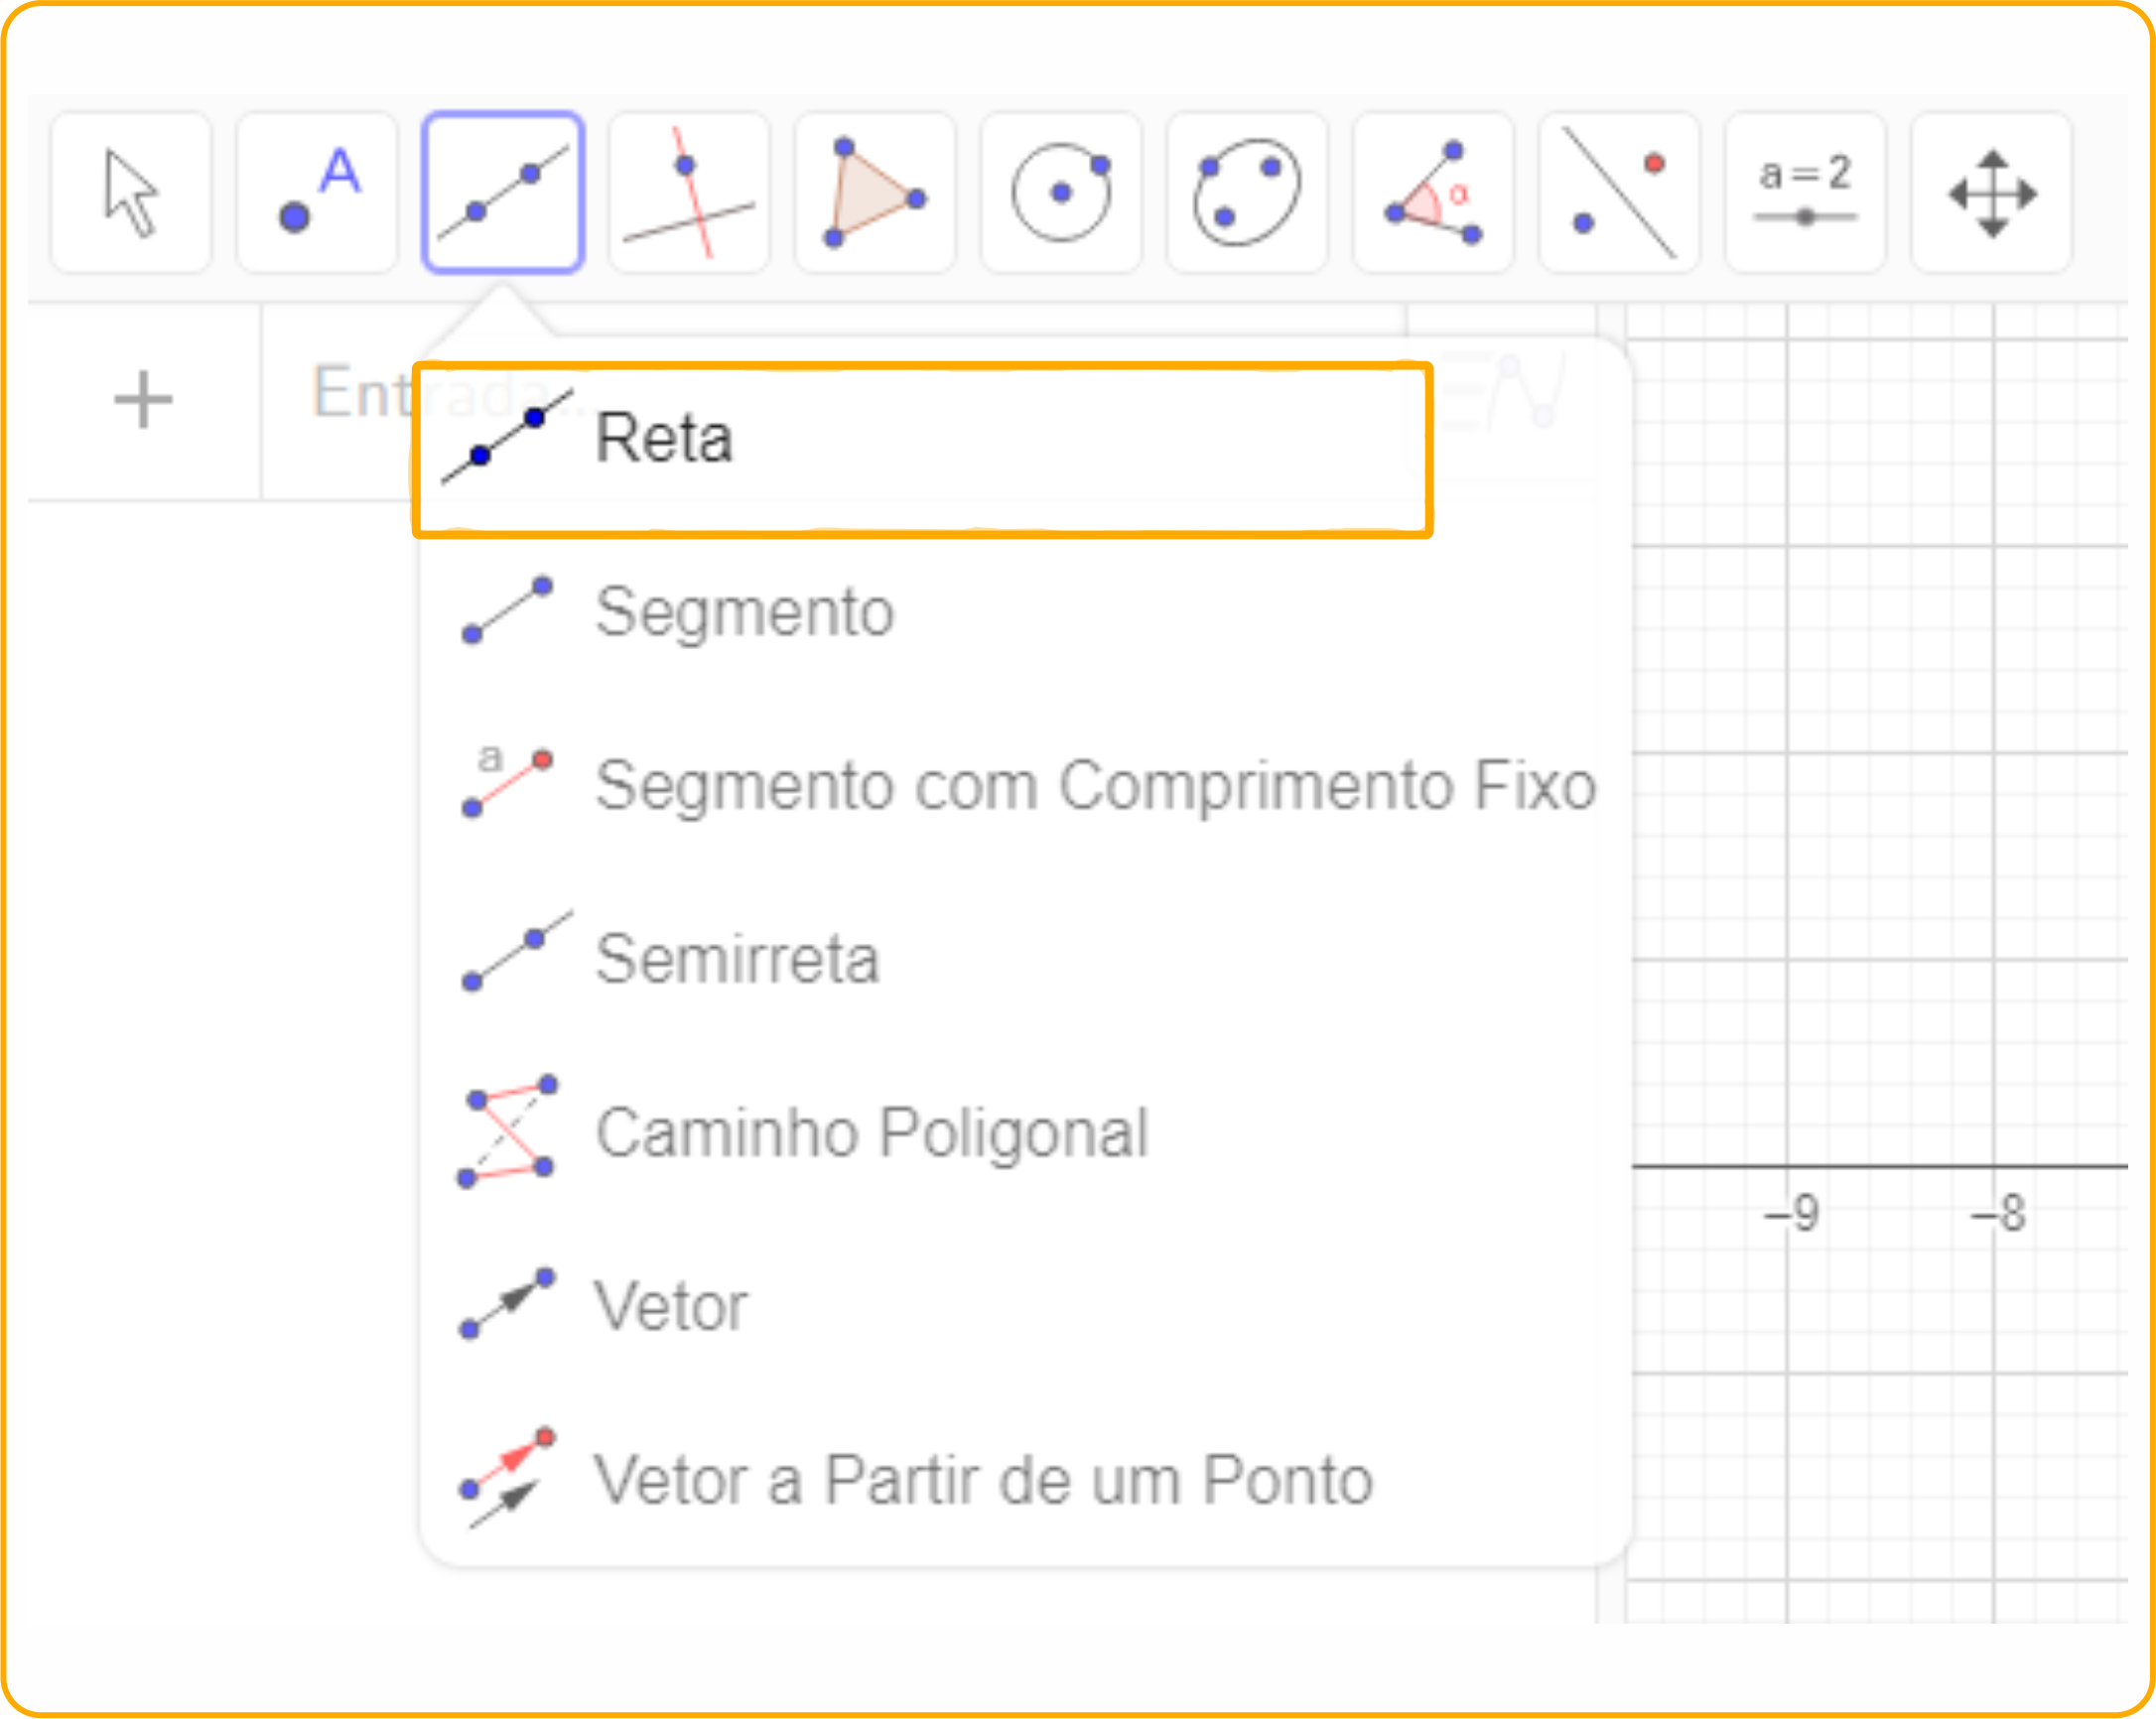
\includegraphics[height=8cm]{Figuras/T01_Elemento02.png}
    \caption{Atividade II - Etapa \ref{Atividade02_Etapa01}}
    \label{Atividade02_Etapa01_Imagem}
\end{figure}

\item Construa a reta $r$ que passe pelos pontos $A$ e $R$, sendo a coordenada do ponto $A (-2,0)$ e do ponto $R (4,1)$.\label{Atividade02_Etapa02}
\begin{figure}[H]
    \centering
    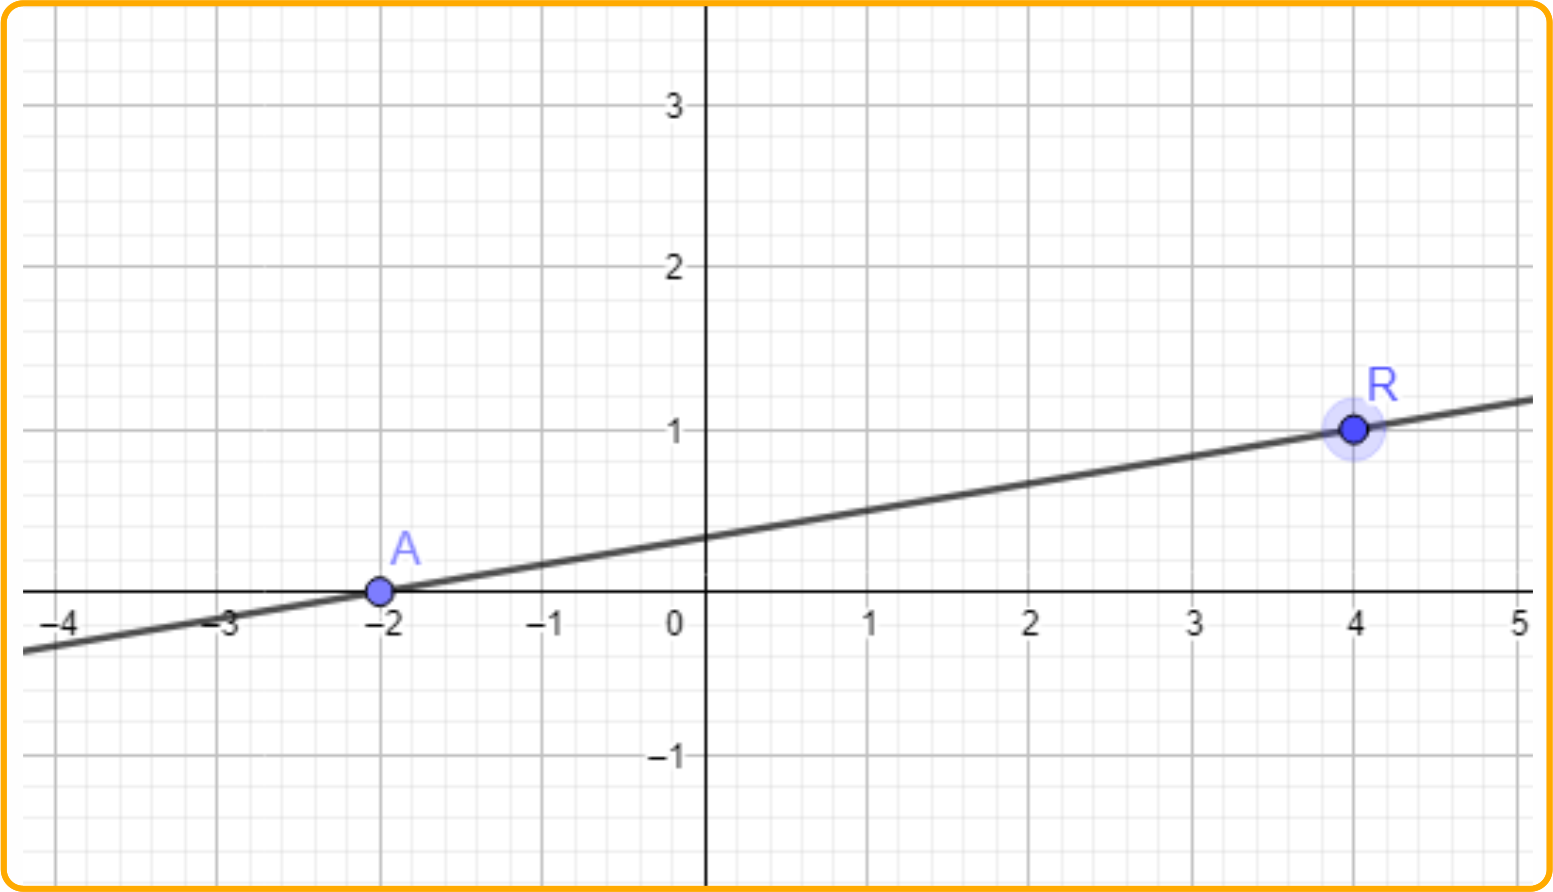
\includegraphics[height=8cm]{Figuras/T01_Atividade02_Fig01.png}
    \caption{Atividade II - Etapa \ref{Atividade02_Etapa02}}
    \label{Atividade02_Etapa02_Imagem}
\end{figure}

\item Selecione o ícone em destaque e clique na opção {\it ponto} \label{Atividade02_Etapa03}
\begin{figure}[H]
    \centering
    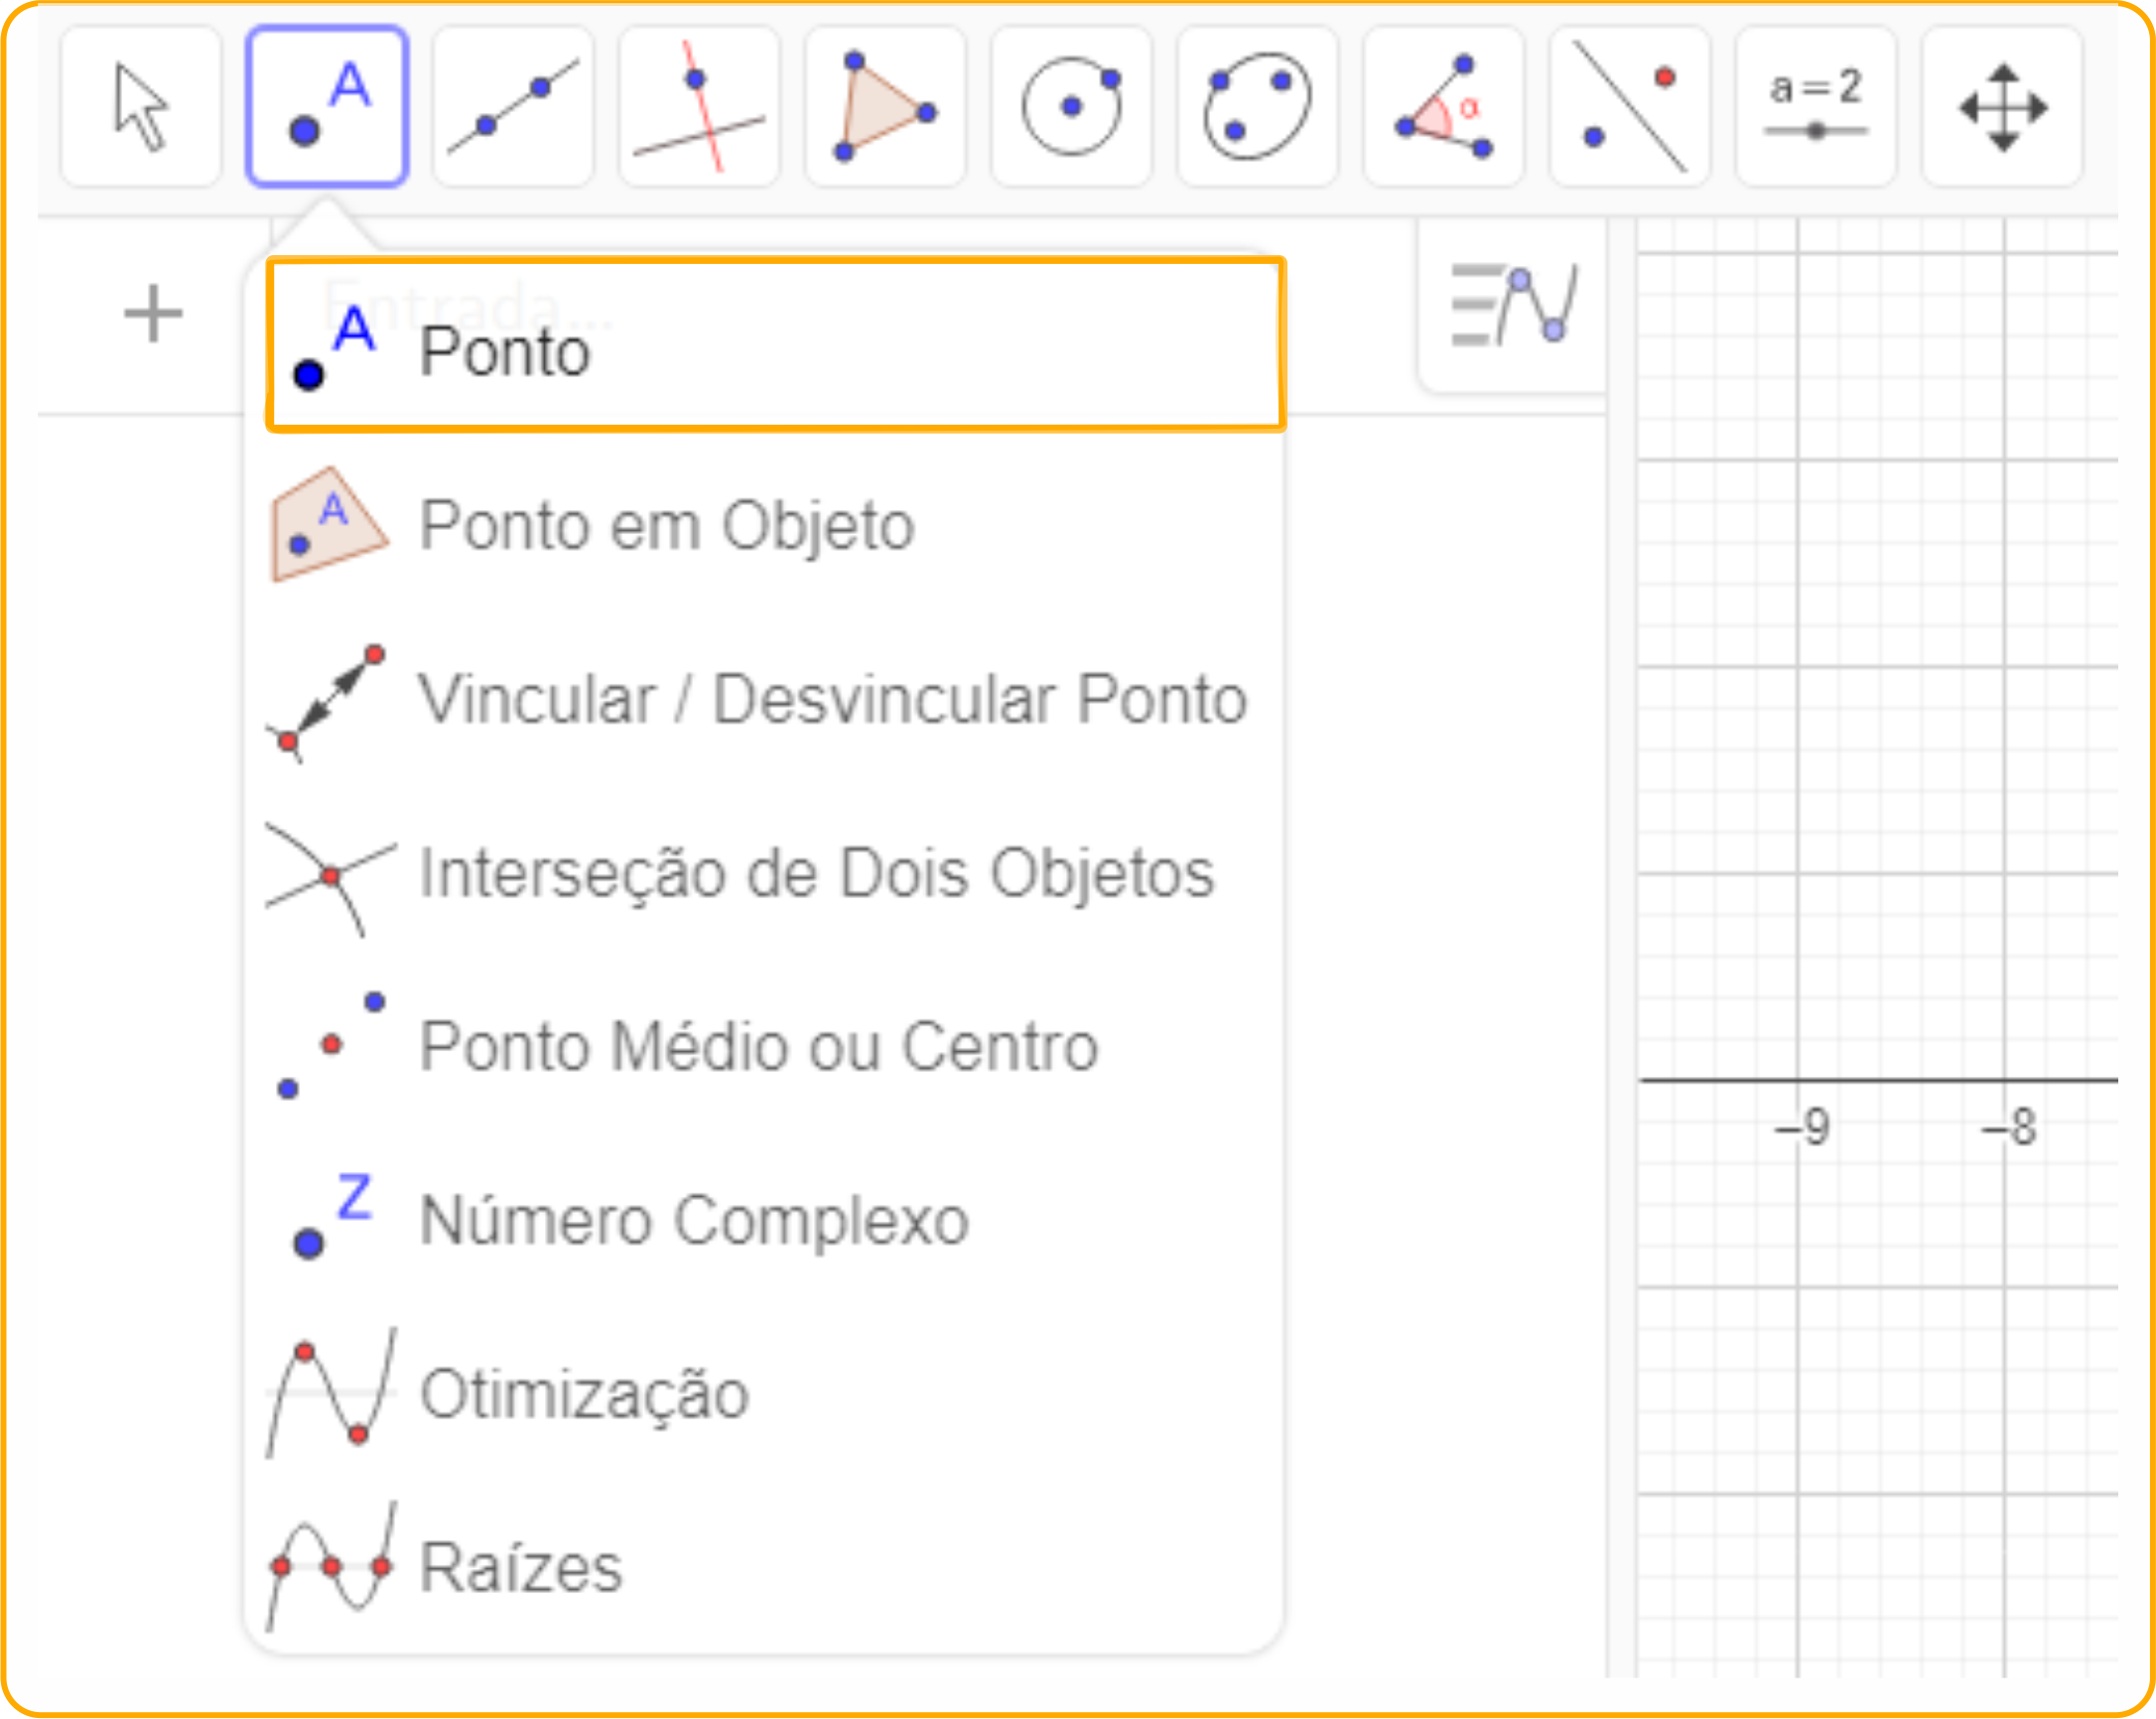
\includegraphics[height=8cm]{Figuras/T01_Elemento01.png}
    \caption{Atividade II - Etapa \ref{Atividade02_Etapa03}}
    \label{Atividade02_Etapa03_Imagem}
\end{figure}

\item Construa o ponto $P$ de coordenada $(-2,2)$ \label{Atividade02_Etapa04}
\begin{figure}[H]
    \centering
    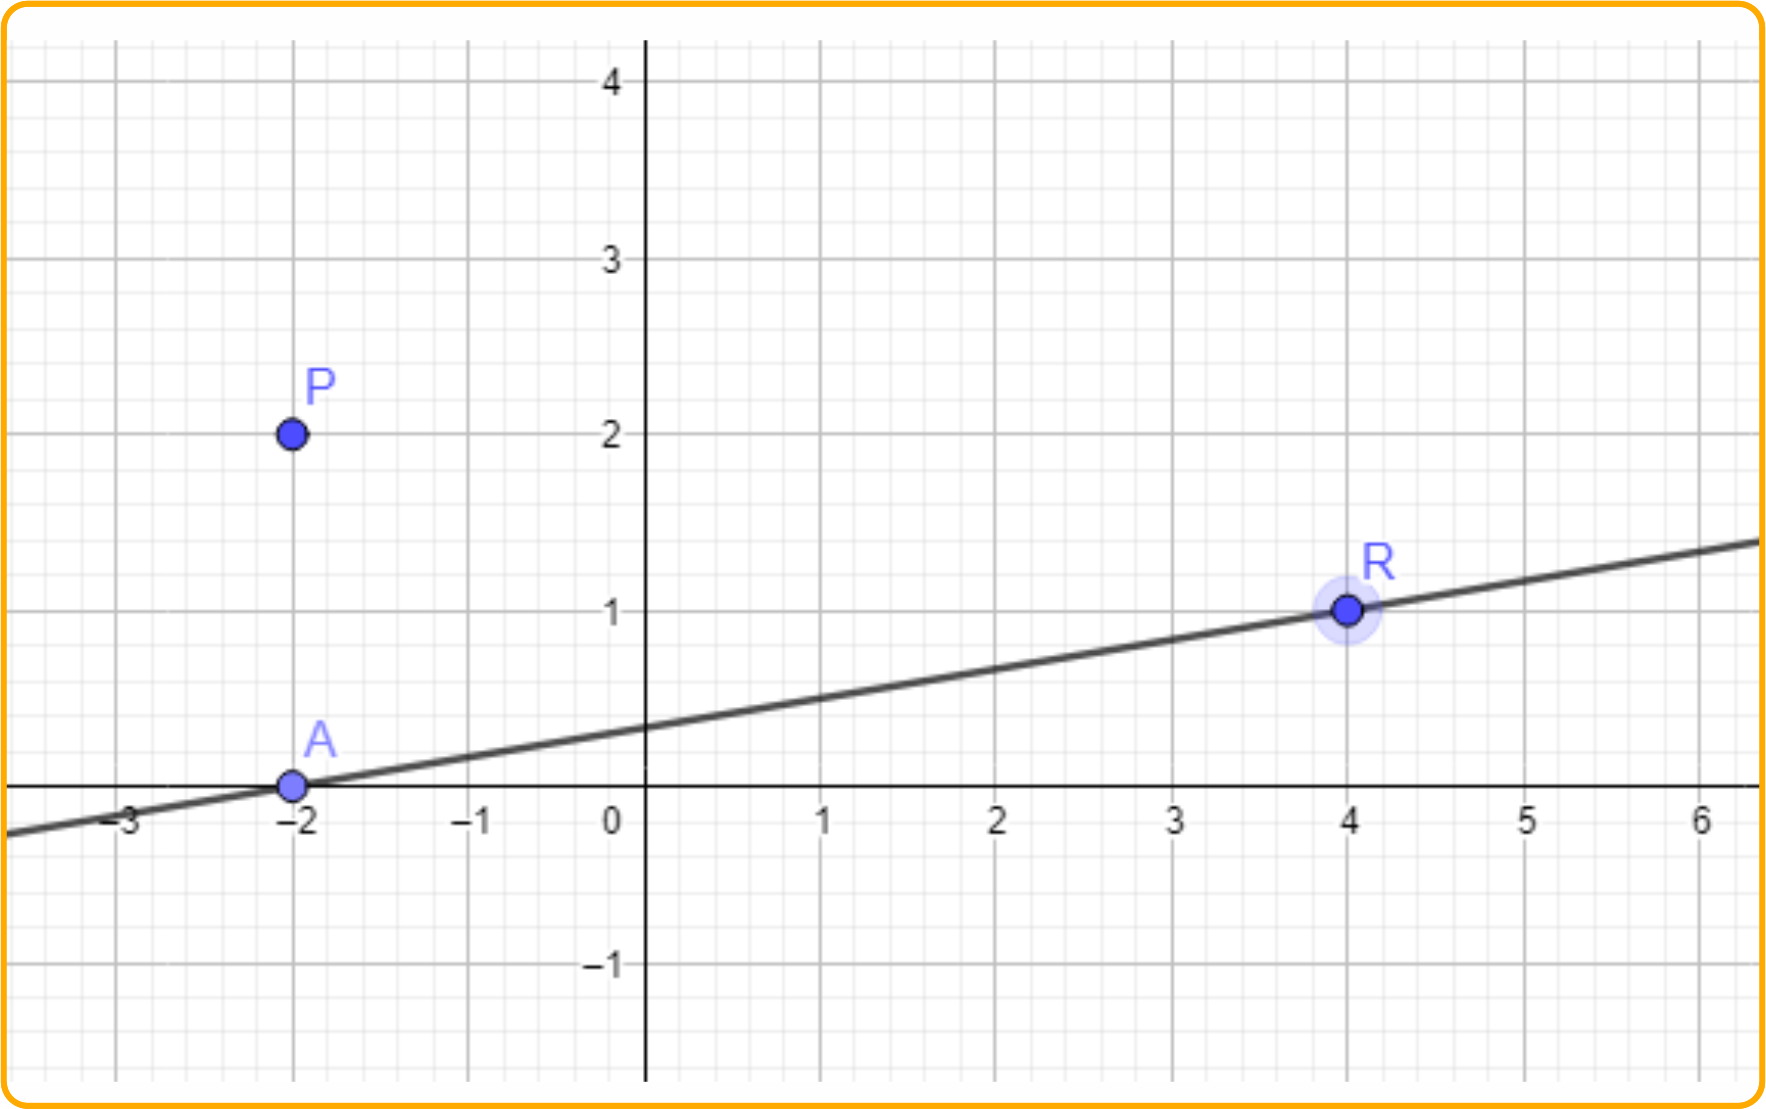
\includegraphics[height=8cm]{Figuras/T01_Atividade02_Fig02.png}
    \caption{Atividade II - Etapa \ref{Atividade02_Etapa04}}
    \label{Atividade02_Etapa04_Imagem}
\end{figure}

\item Selecione o ícone em destaque e clique na opção {\it círculo: centro \& raio} \label{Atividade02_Etapa05}
\begin{figure}[H]
    \centering
    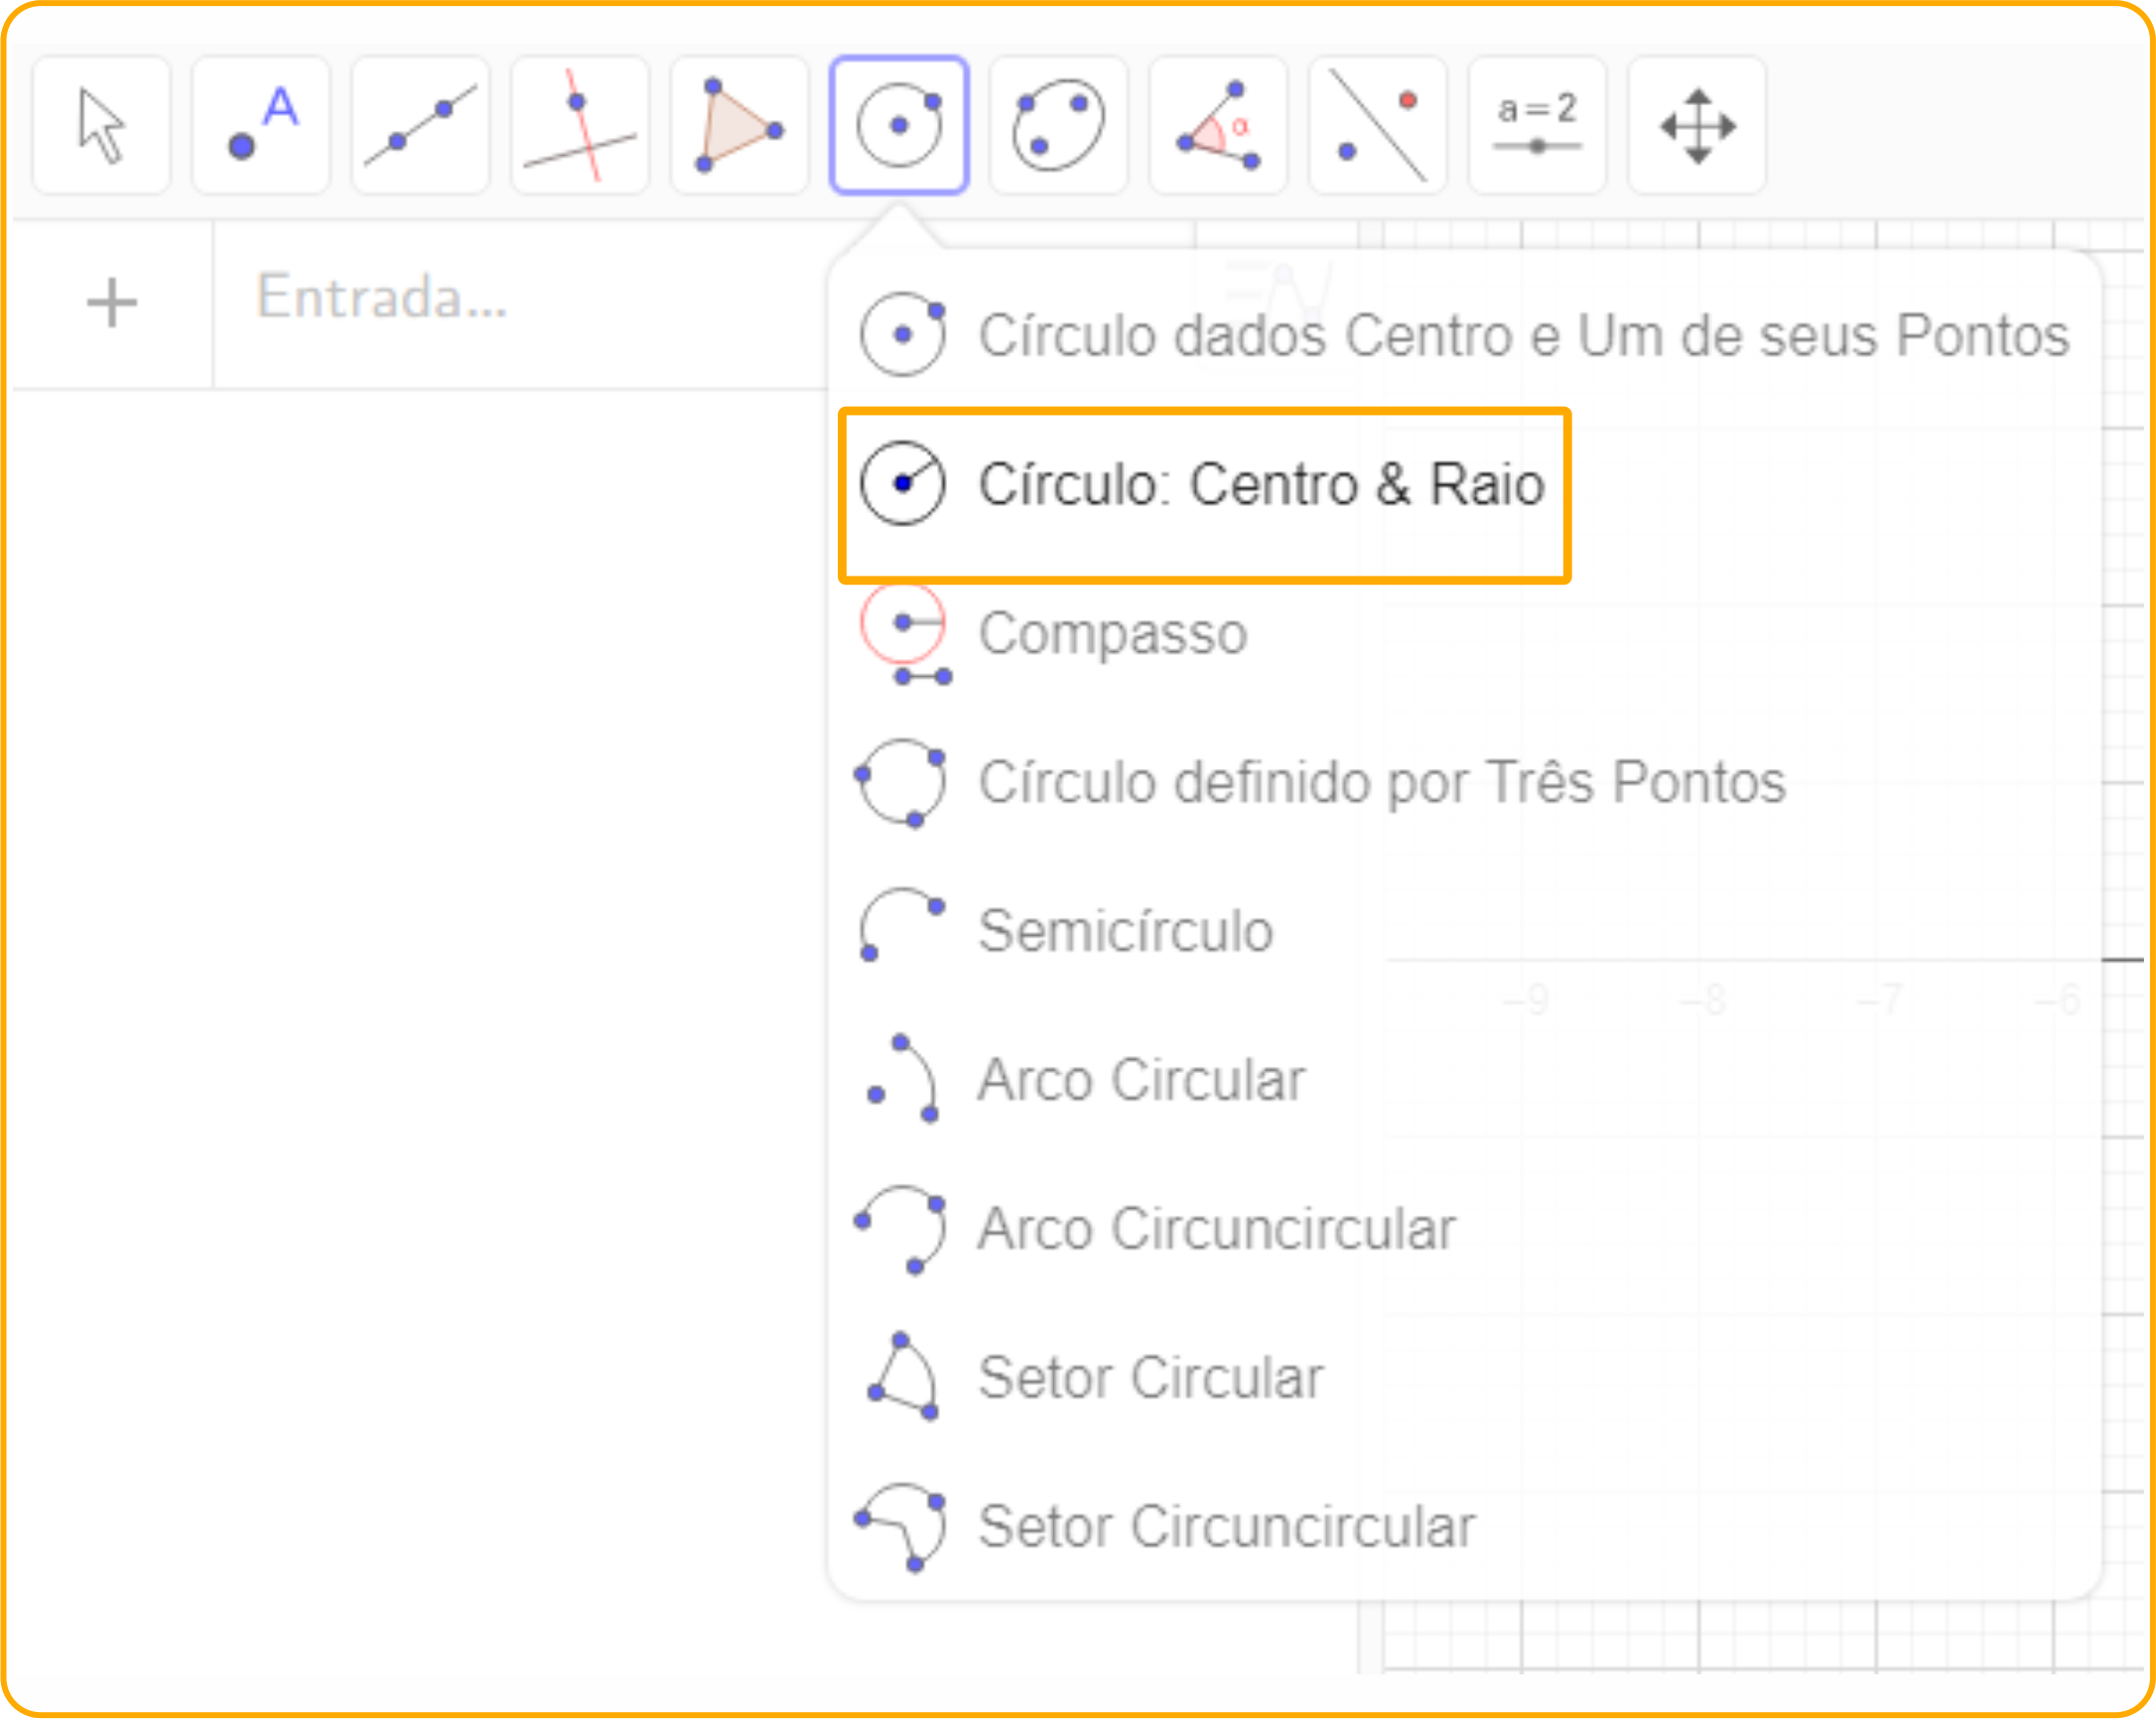
\includegraphics[height=8cm]{Figuras/T01_Elemento07.png}
    \caption{Atividade II - Etapa \ref{Atividade02_Etapa05}}
    \label{Atividade02_Etapa05_Imagem}
\end{figure}

\item Selecione o ponto ${\color{blue}{P}}$ e trace a circunferência ${\color{red}{c}}$ de raio $3$ \label{Atividade02_Etapa06}
\begin{figure}[H]
    \centering
    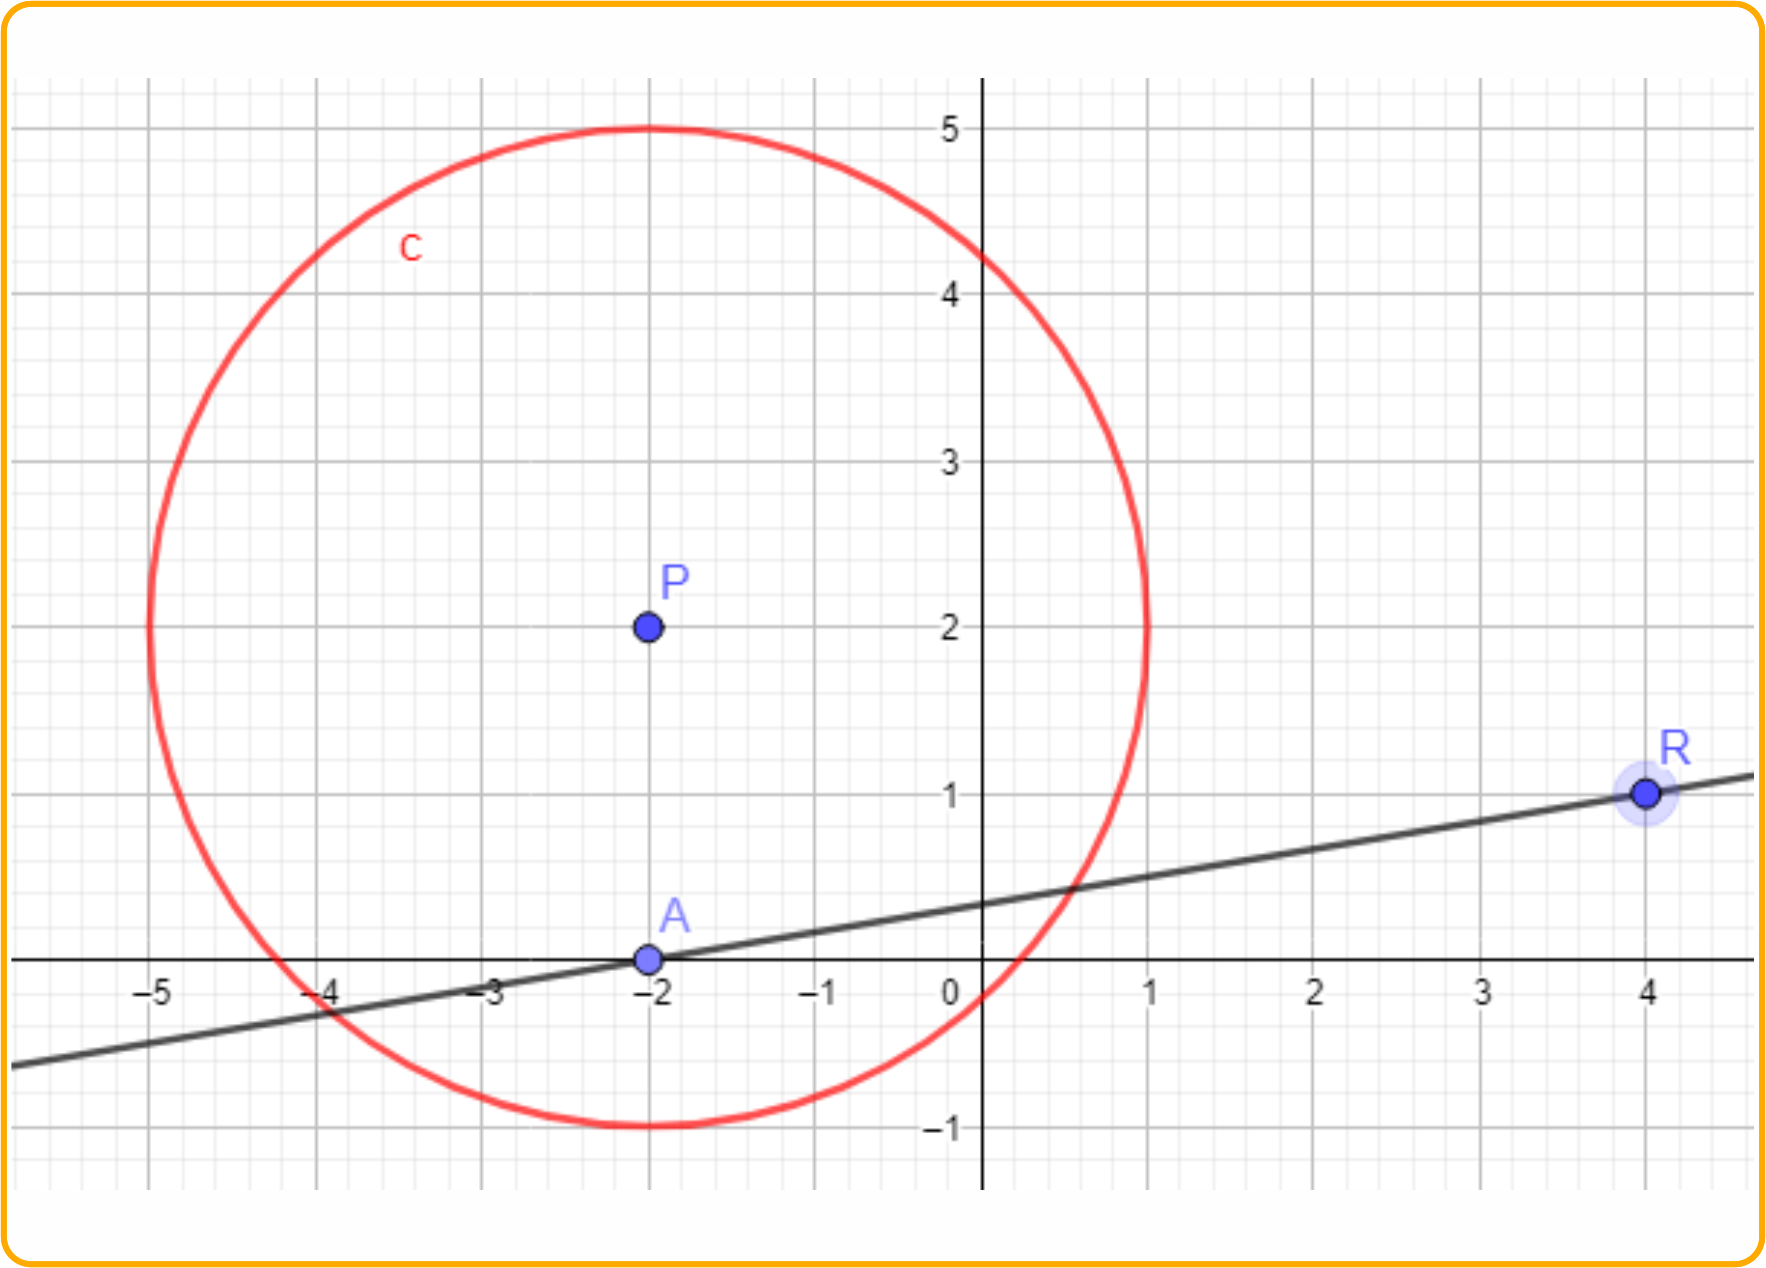
\includegraphics[height=8cm]{Figuras/T01_Atividade02_Fig03.png}
    \caption{Atividade II - Etapa \ref{Atividade02_Etapa06}}
    \label{Atividade02_Etapa06_Imagem}
\end{figure}

\item Selecione o ícone em destaque e clique na opção {\it interseção de dois objetos} \label{Atividade02_Etapa07}
\begin{figure}[H]
    \centering
    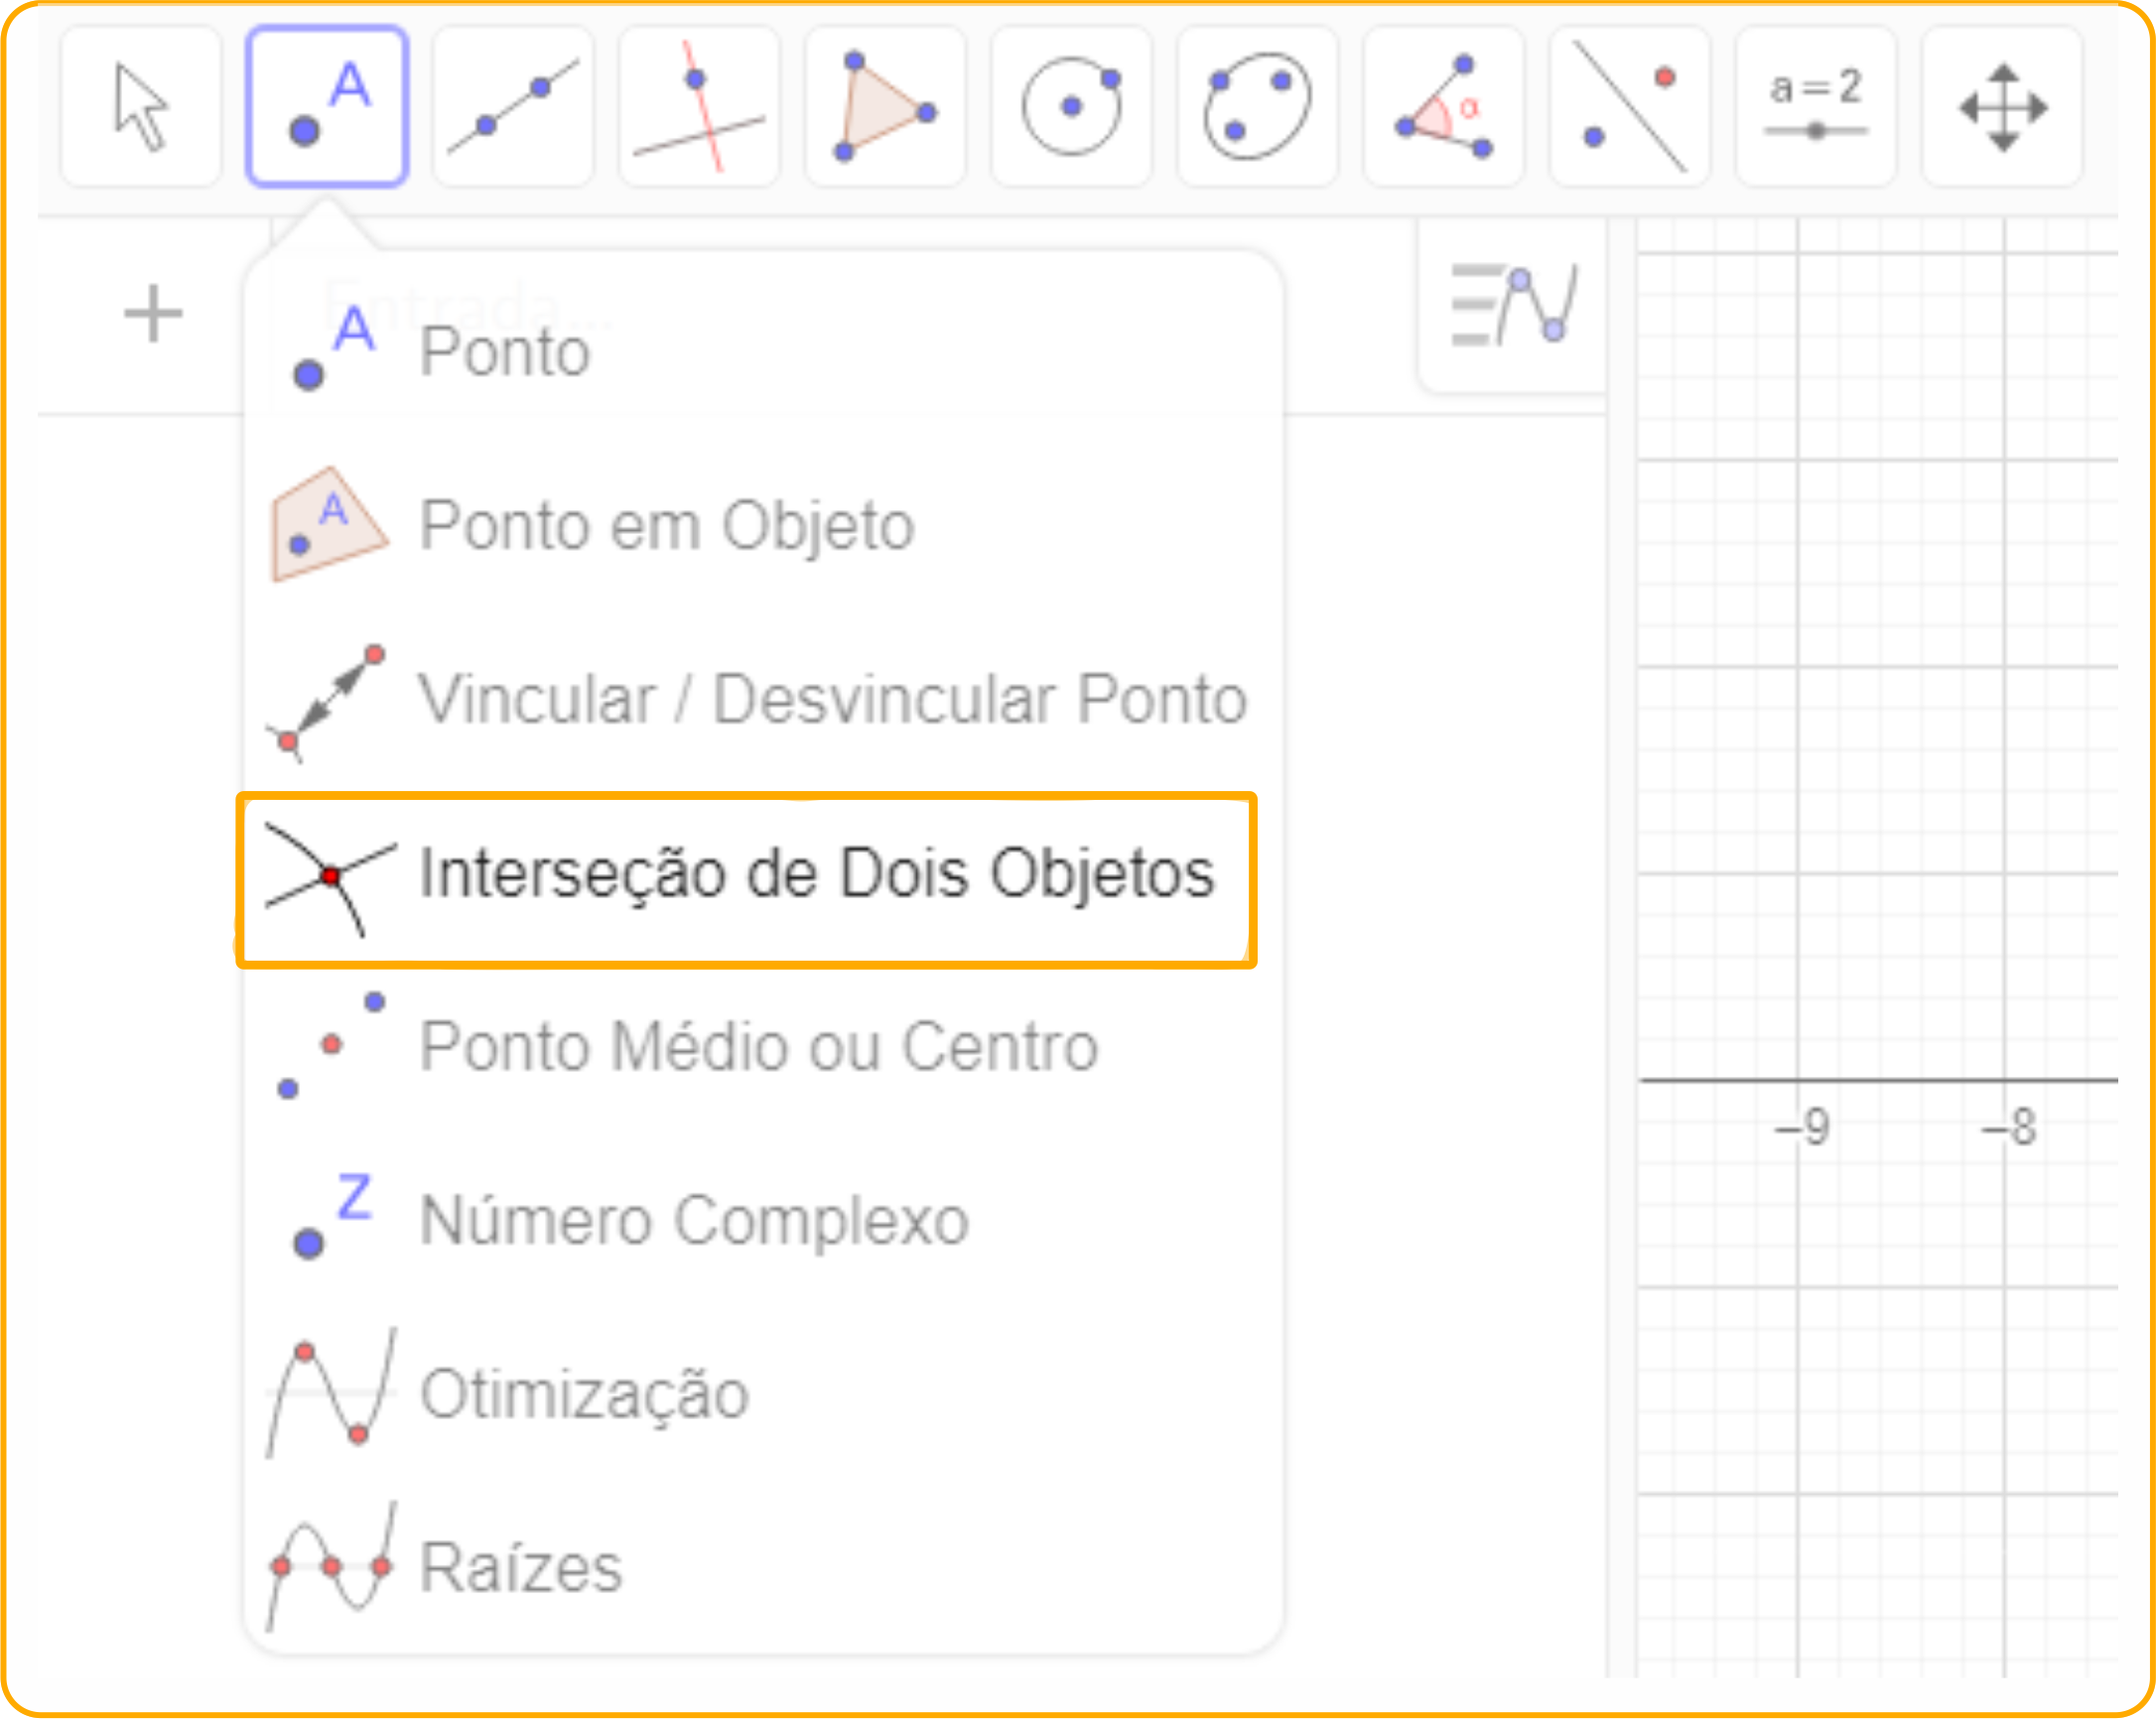
\includegraphics[height=8cm]{Figuras/T01_Elemento05.png}
    \caption{Atividade II - Etapa \ref{Atividade02_Etapa07}}
    \label{Atividade02_Etapa07_Imagem}
\end{figure}

\item Construa o ponto $B$ na interseção da circunferência ${\color{red}{c}}$ com a reta $r$. \label{Atividade02_Etapa08}
\begin{figure}[H]
    \centering
    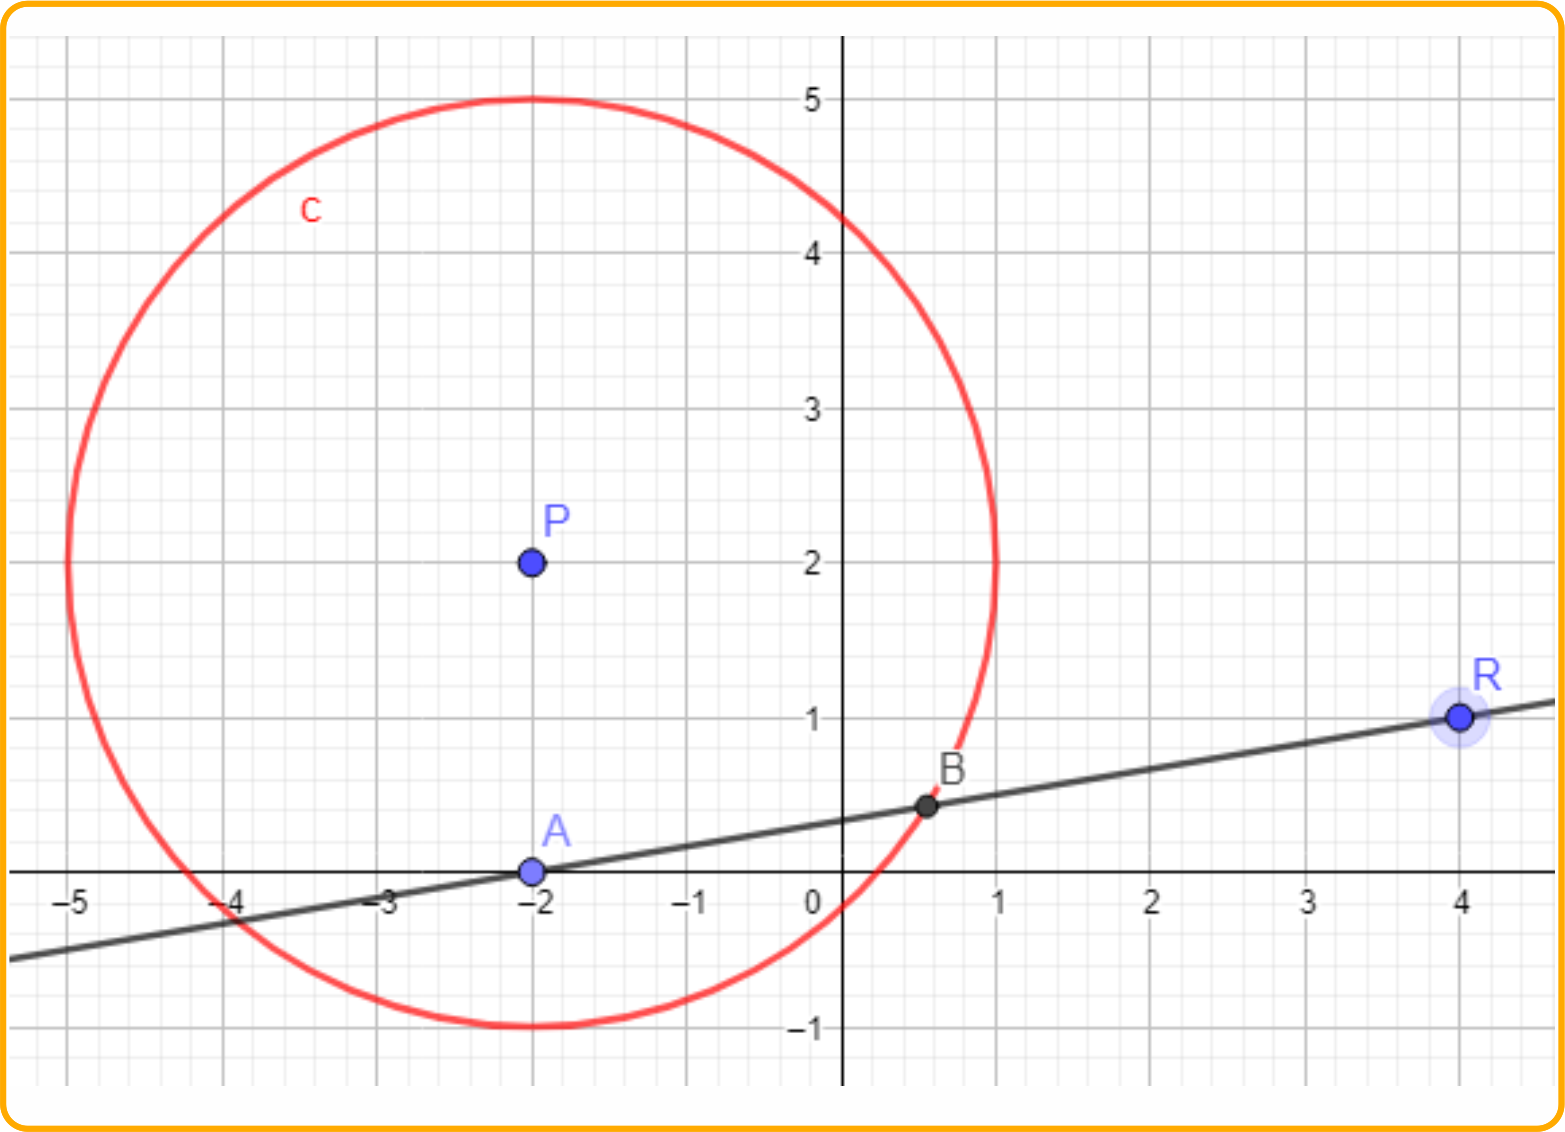
\includegraphics[height=8cm]{Figuras/T01_Atividade02_Fig04.png}
    \caption{Atividade II - Etapa \ref{Atividade02_Etapa08}}
    \label{Atividade02_Etapa08_Imagem}
\end{figure}

\item Selecione o ícone em destaque e clique na opção {\it compasso} \label{Atividade02_Etapa09}
\begin{figure}[H]
    \centering
    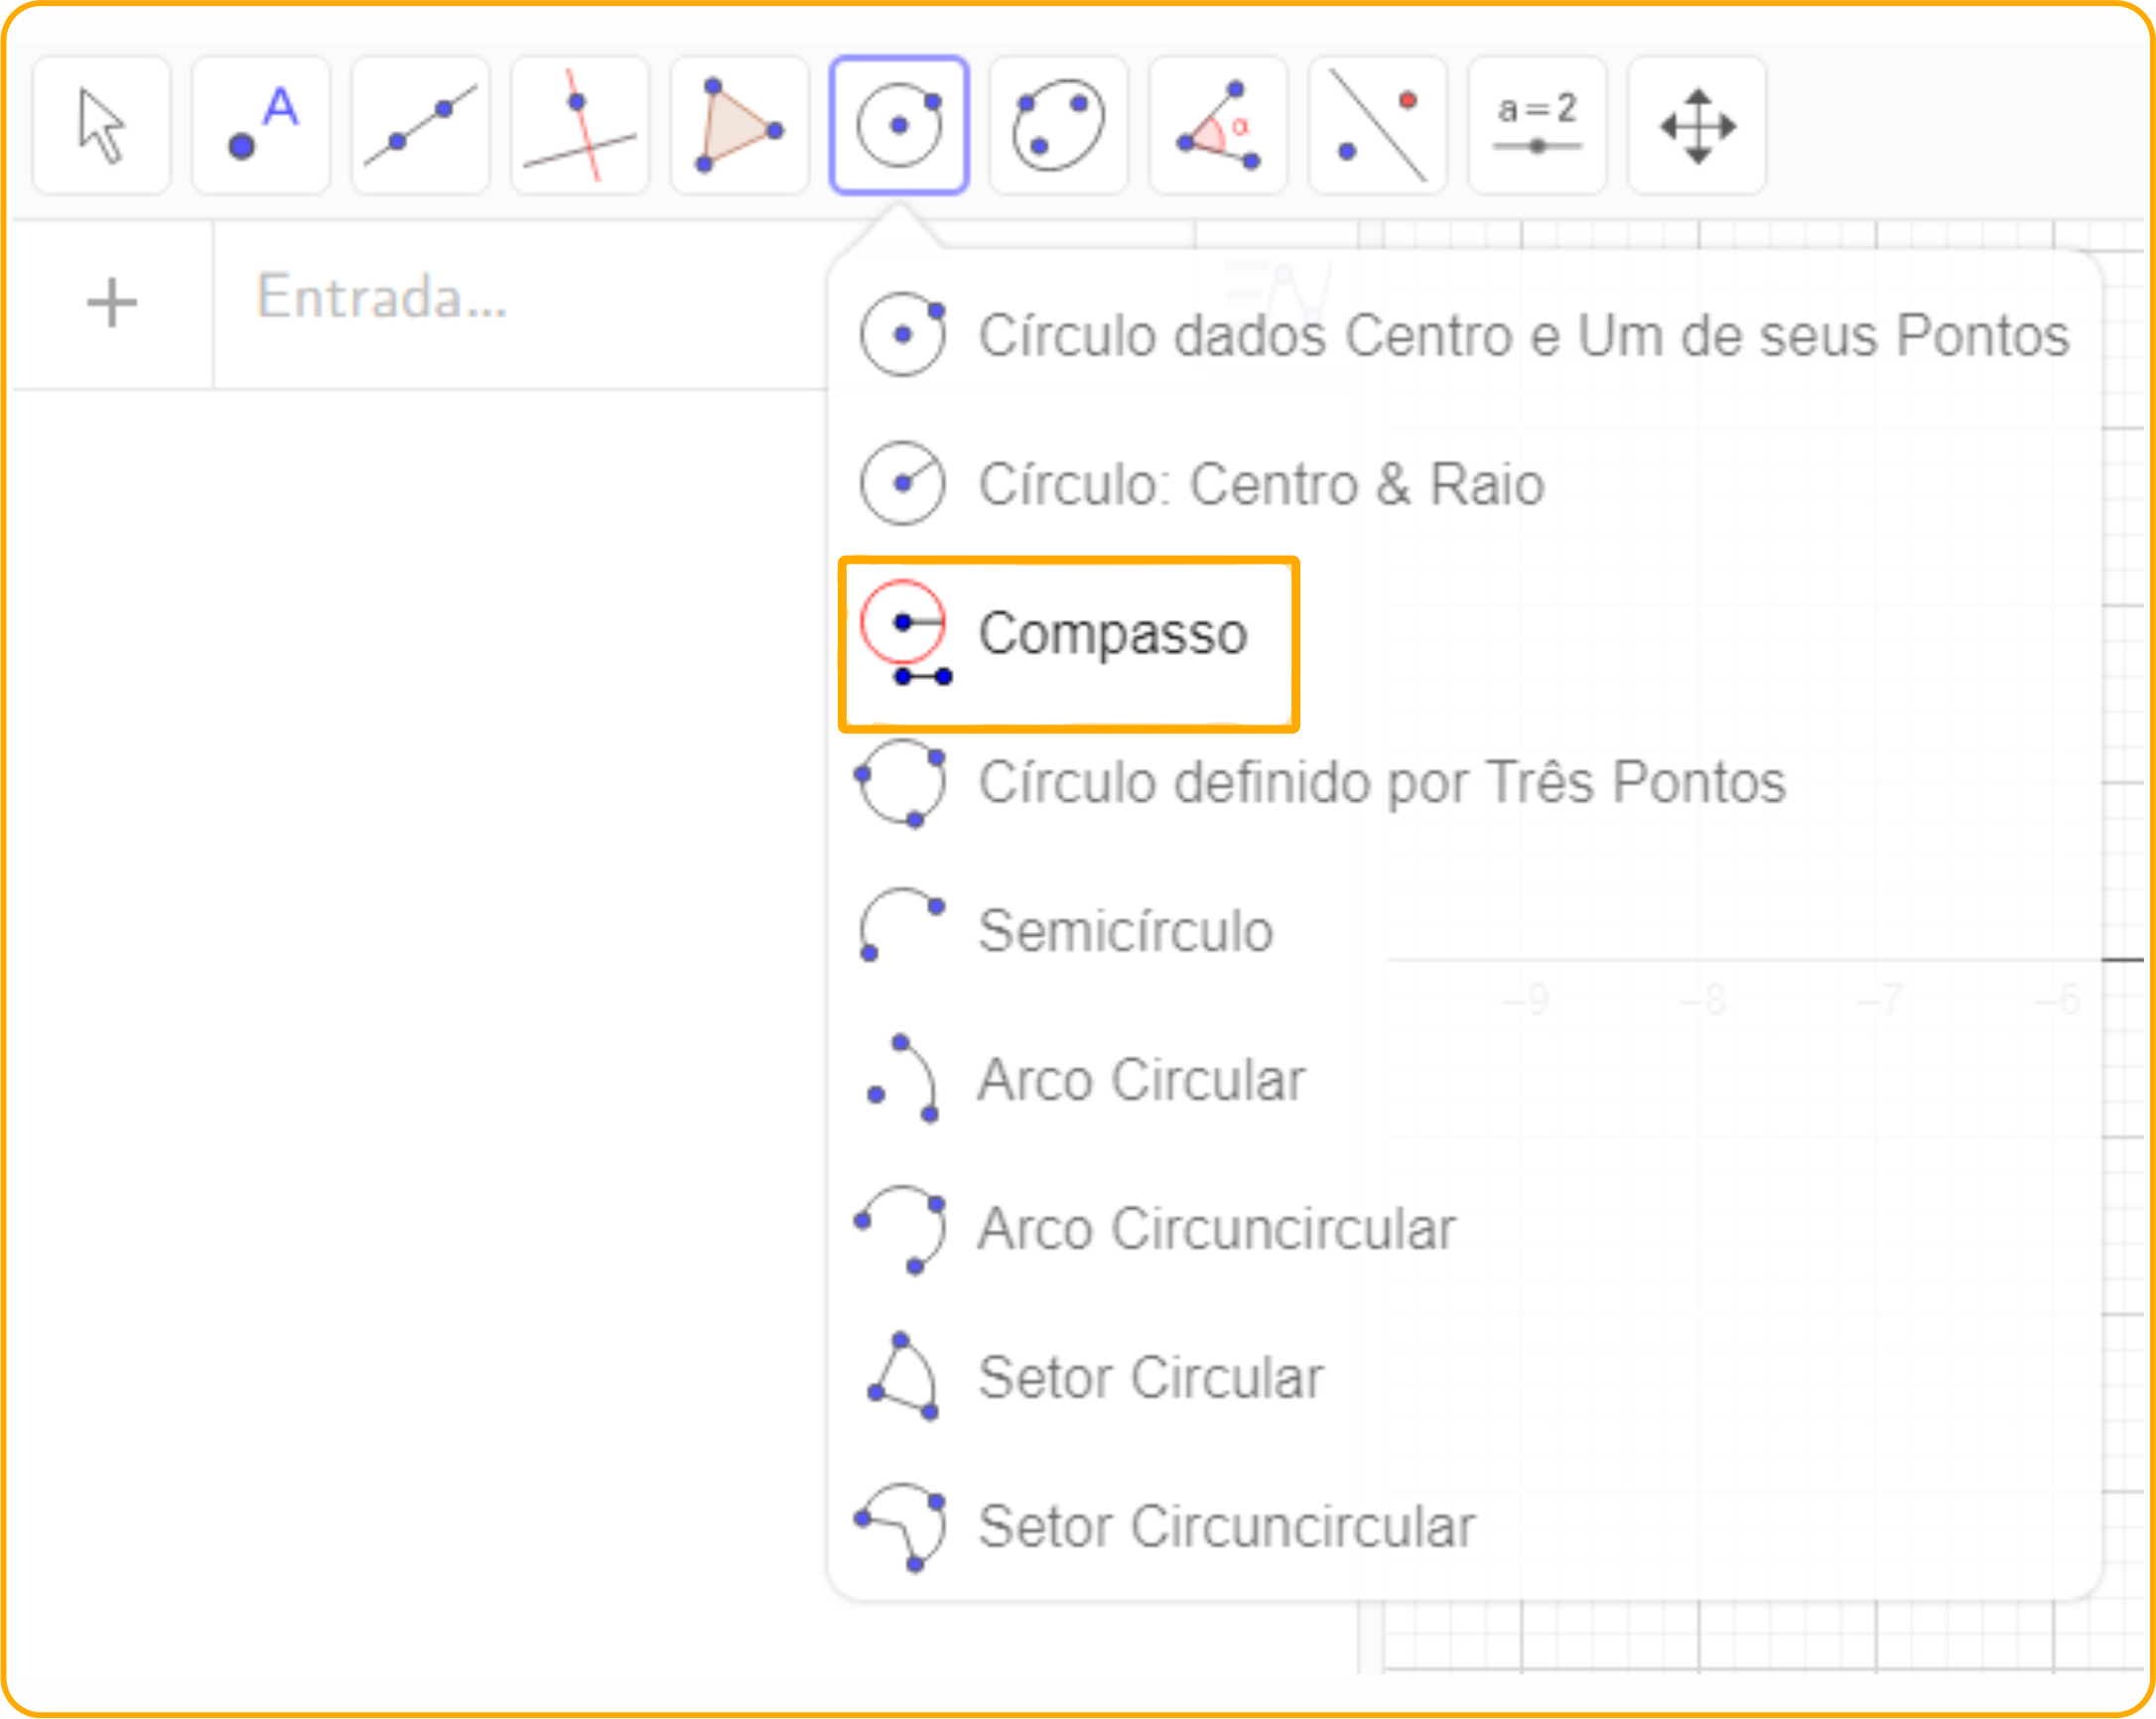
\includegraphics[height=8cm]{Figuras/T01_Elemento04.png}
    \caption{Atividade II - Etapa \ref{Atividade02_Etapa09}}
    \label{Atividade02_Etapa09_Imagem}
\end{figure}

\item Construa uma circunferência ${\color{blue}{d}}$  com centro no ponto $B$ e com raio de mesma medida que o segmento $\overline{PB}$. \label{Atividade02_Etapa10}
\begin{figure}[H]
    \centering
    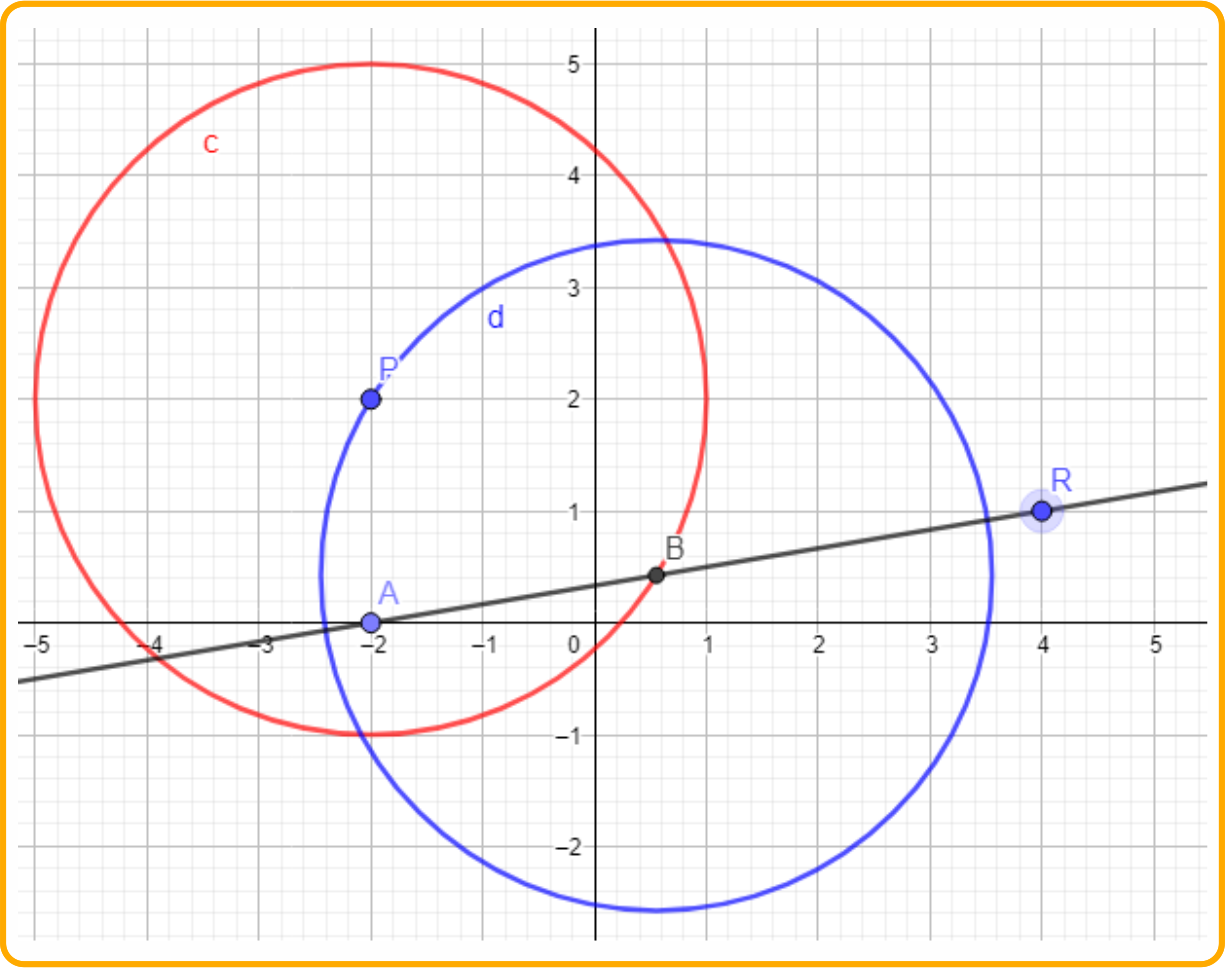
\includegraphics[height=8cm]{Figuras/T01_Atividade02_Fig05.png}
    \caption{Atividade II - Etapa \ref{Atividade02_Etapa10}}
    \label{Atividade02_Etapa10_Imagem}
\end{figure}

\item Repita a Etapa \ref{Atividade02_Etapa07} e marque o ponto $C$ na interseção entre a circunferência ${\color{blue}{d}}$  e a reta $r$ \label{Atividade02_Etapa11}
\begin{figure}[H]
    \centering
    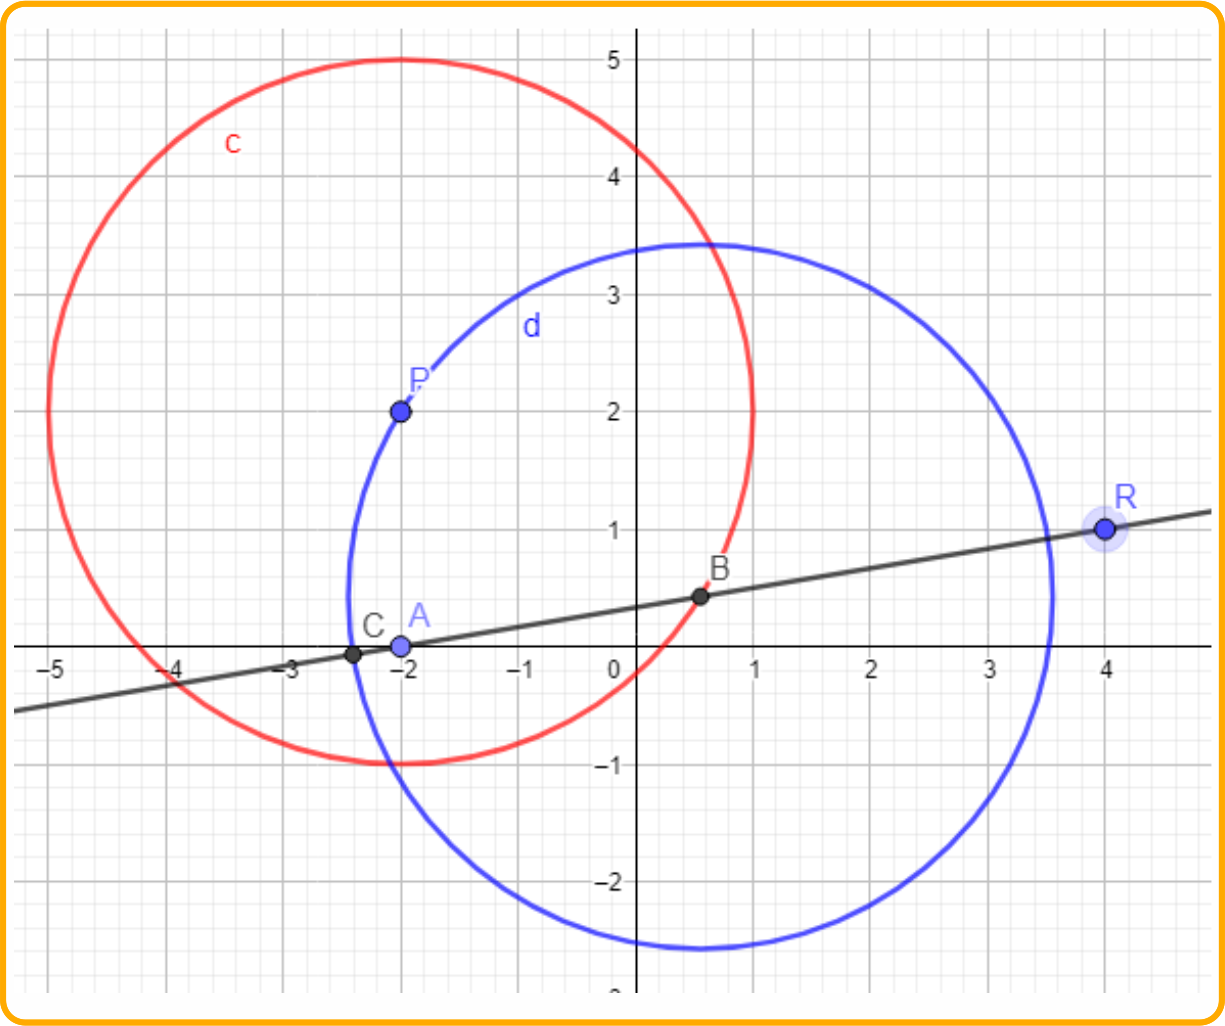
\includegraphics[height=8cm]{Figuras/T01_Atividade02_Fig06.png}
    \caption{Atividade II - Etapa \ref{Atividade02_Etapa11}}
    \label{Atividade02_Etapa11_Imagem}
\end{figure}

\item Repita a Etapa \ref{Atividade02_Etapa10} e construa uma circunferência ${\color{ForestGreen}{e}}$ com centro no ponto $B$ e com raio de mesma medida que o segmento $\overline{PC}$ \label{Atividade02_Etapa12}
\begin{figure}[H]
    \centering
    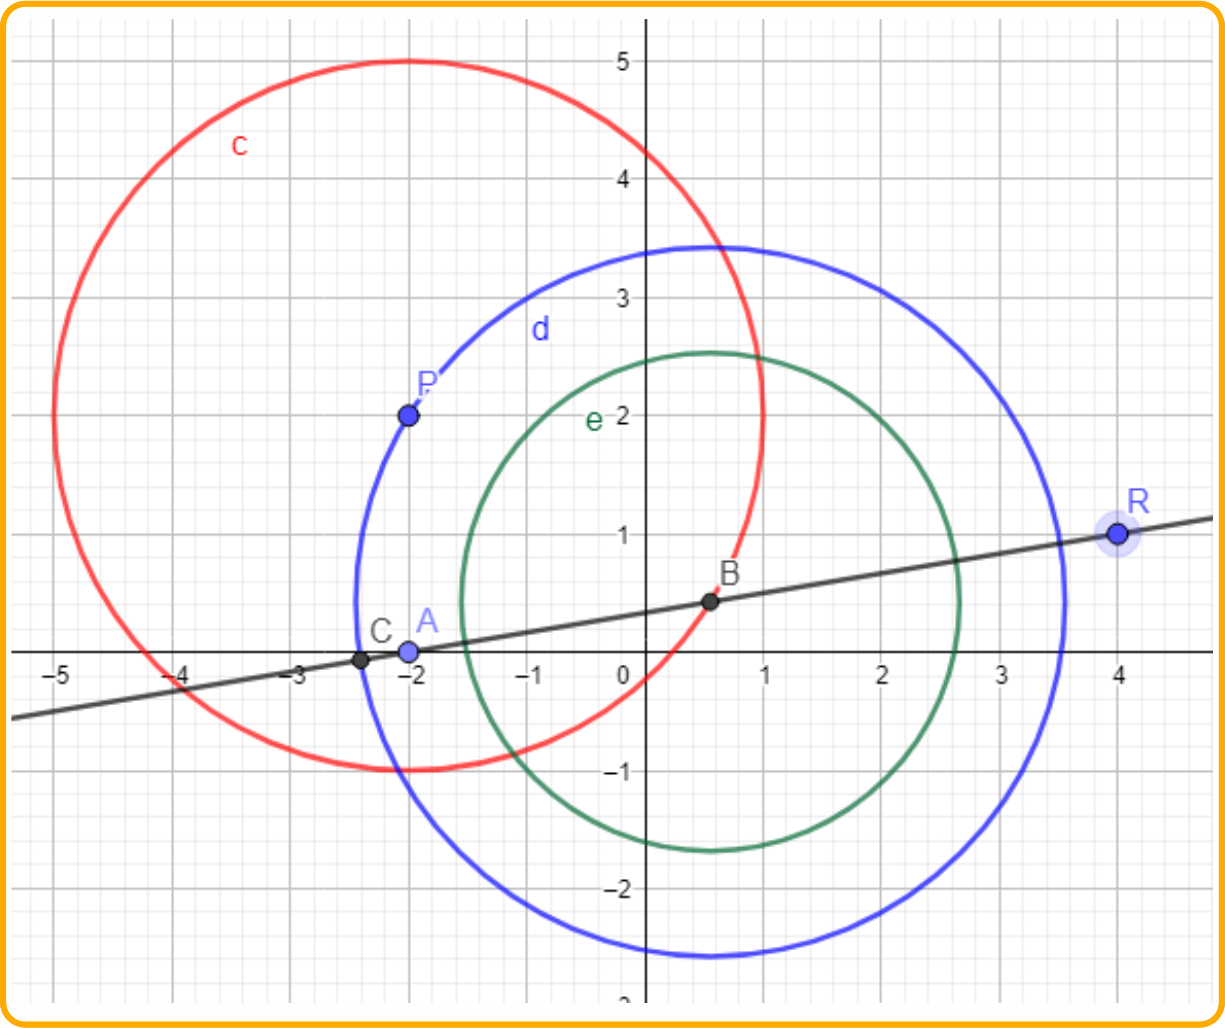
\includegraphics[height=8cm]{Figuras/T01_Atividade02_Fig07.png}
    \caption{Atividade II - Etapa \ref{Atividade02_Etapa12}}
    \label{Atividade02_Etapa12_Imagem}
\end{figure}

\item Repita a Etapa \ref{Atividade02_Etapa07} e marque o ponto $D$ na interseção entre as circunferências ${\color{red}{c}}$  e ${\color{ForestGreen}{e}}$ \label{Atividade02_Etapa13}
\begin{figure}[H]
    \centering
    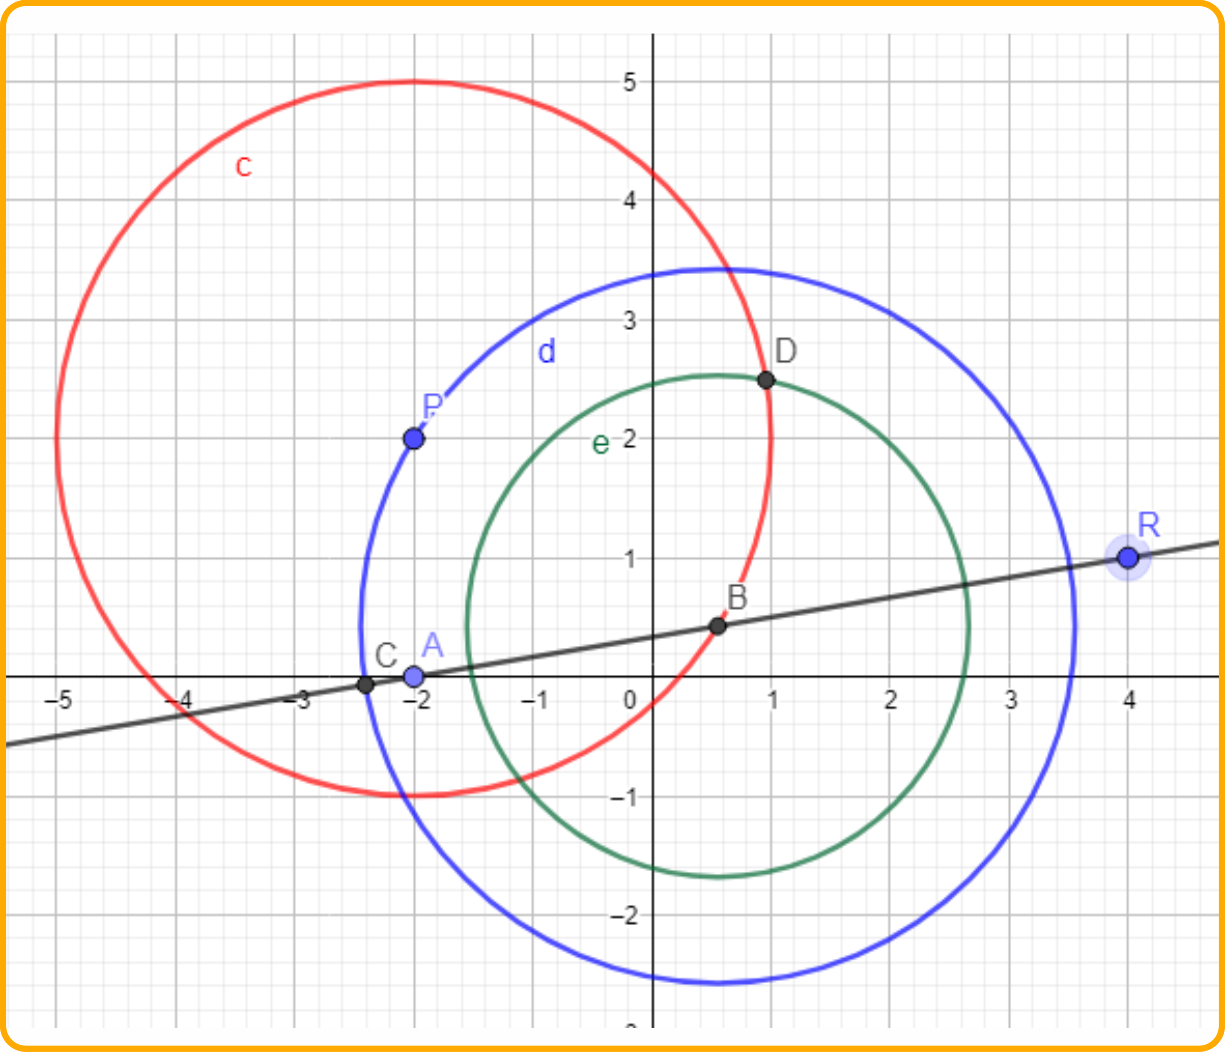
\includegraphics[height=8cm]{Figuras/T01_Atividade02_Fig08.png}
    \caption{Atividade II - Etapa \ref{Atividade02_Etapa13}}
    \label{Atividade02_Etapa13_Imagem}
\end{figure}

\item Repita a Etapa \ref{Atividade02_Etapa01} e construa a reta ${\color{magenta}{s}}$ , que passa pelos pontos $P$ e $D$. \label{Atividade02_Etapa14}
\begin{figure}[H]
    \centering
    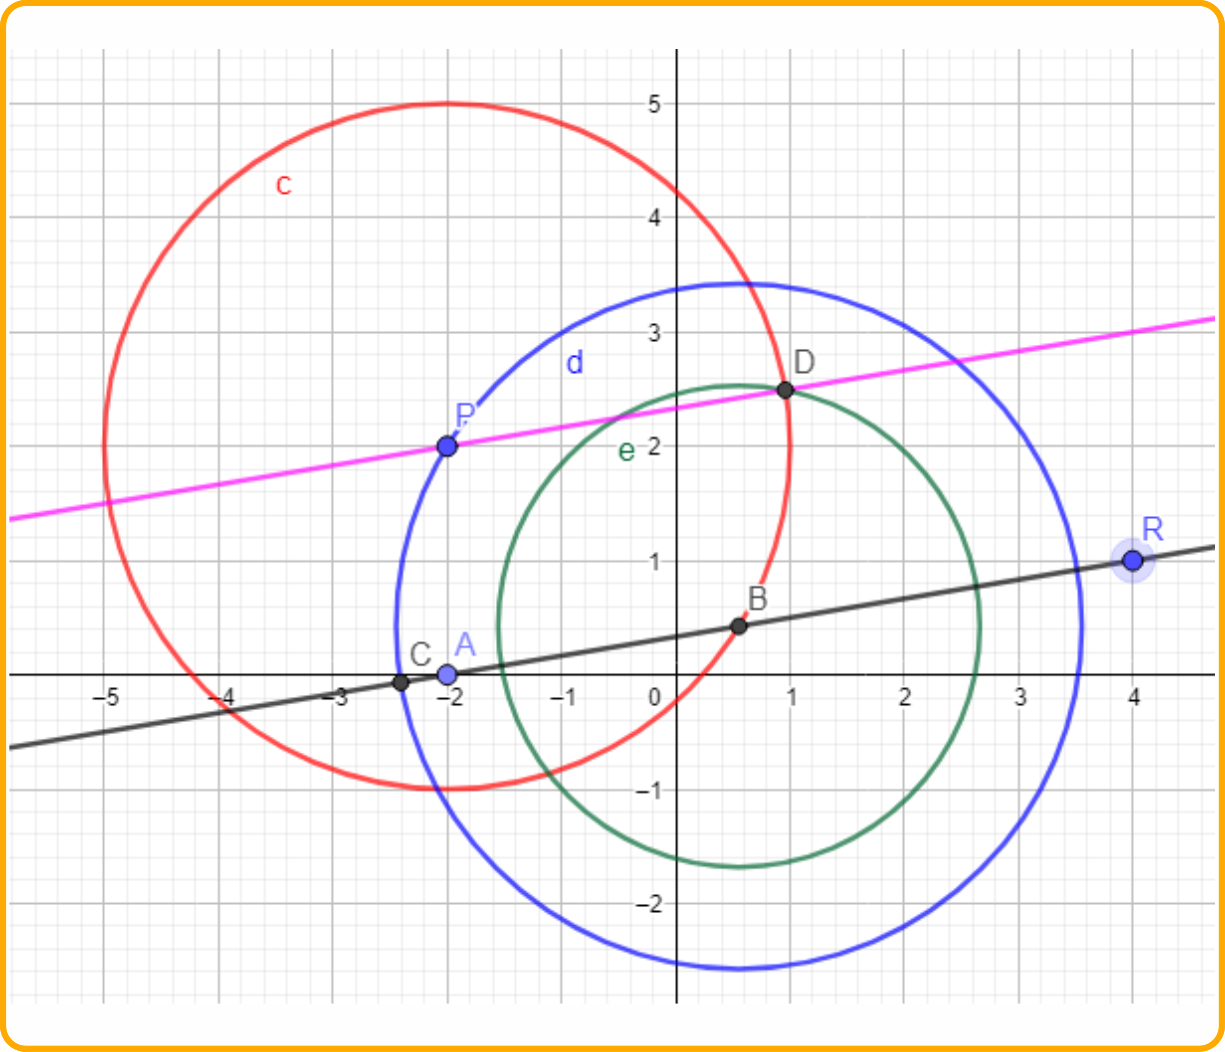
\includegraphics[height=8cm]{Figuras/T01_Atividade02_Fig09.png}
    \caption{Atividade II - Etapa \ref{Atividade02_Etapa14}}
    \label{Atividade02_Etapa14_Imagem}
\end{figure}
\end{enumerate}
A reta ${\color{magenta}{s}}$  será paralela à $r$, pois da forma como foi feita a construção, PCBD é um losango e portanto seus lados $\overline{PD}$ e $\overline{CB}$ são paralelos.

\newpage

%%%%%%% SUBSEÇÃO 03 - ATIVIDADE 03 %%%%%%%%
\subsection{Atividade III: Construção de uma reta perpendicular a uma reta dada que passe por um ponto exterior}

\begin{enumerate}[{Etapa} 1.]
\item Selecione o ícone em destaque e clique na opção {\it reta} \label{Atividade03_Etapa01}
\begin{figure}[H]
    \centering
    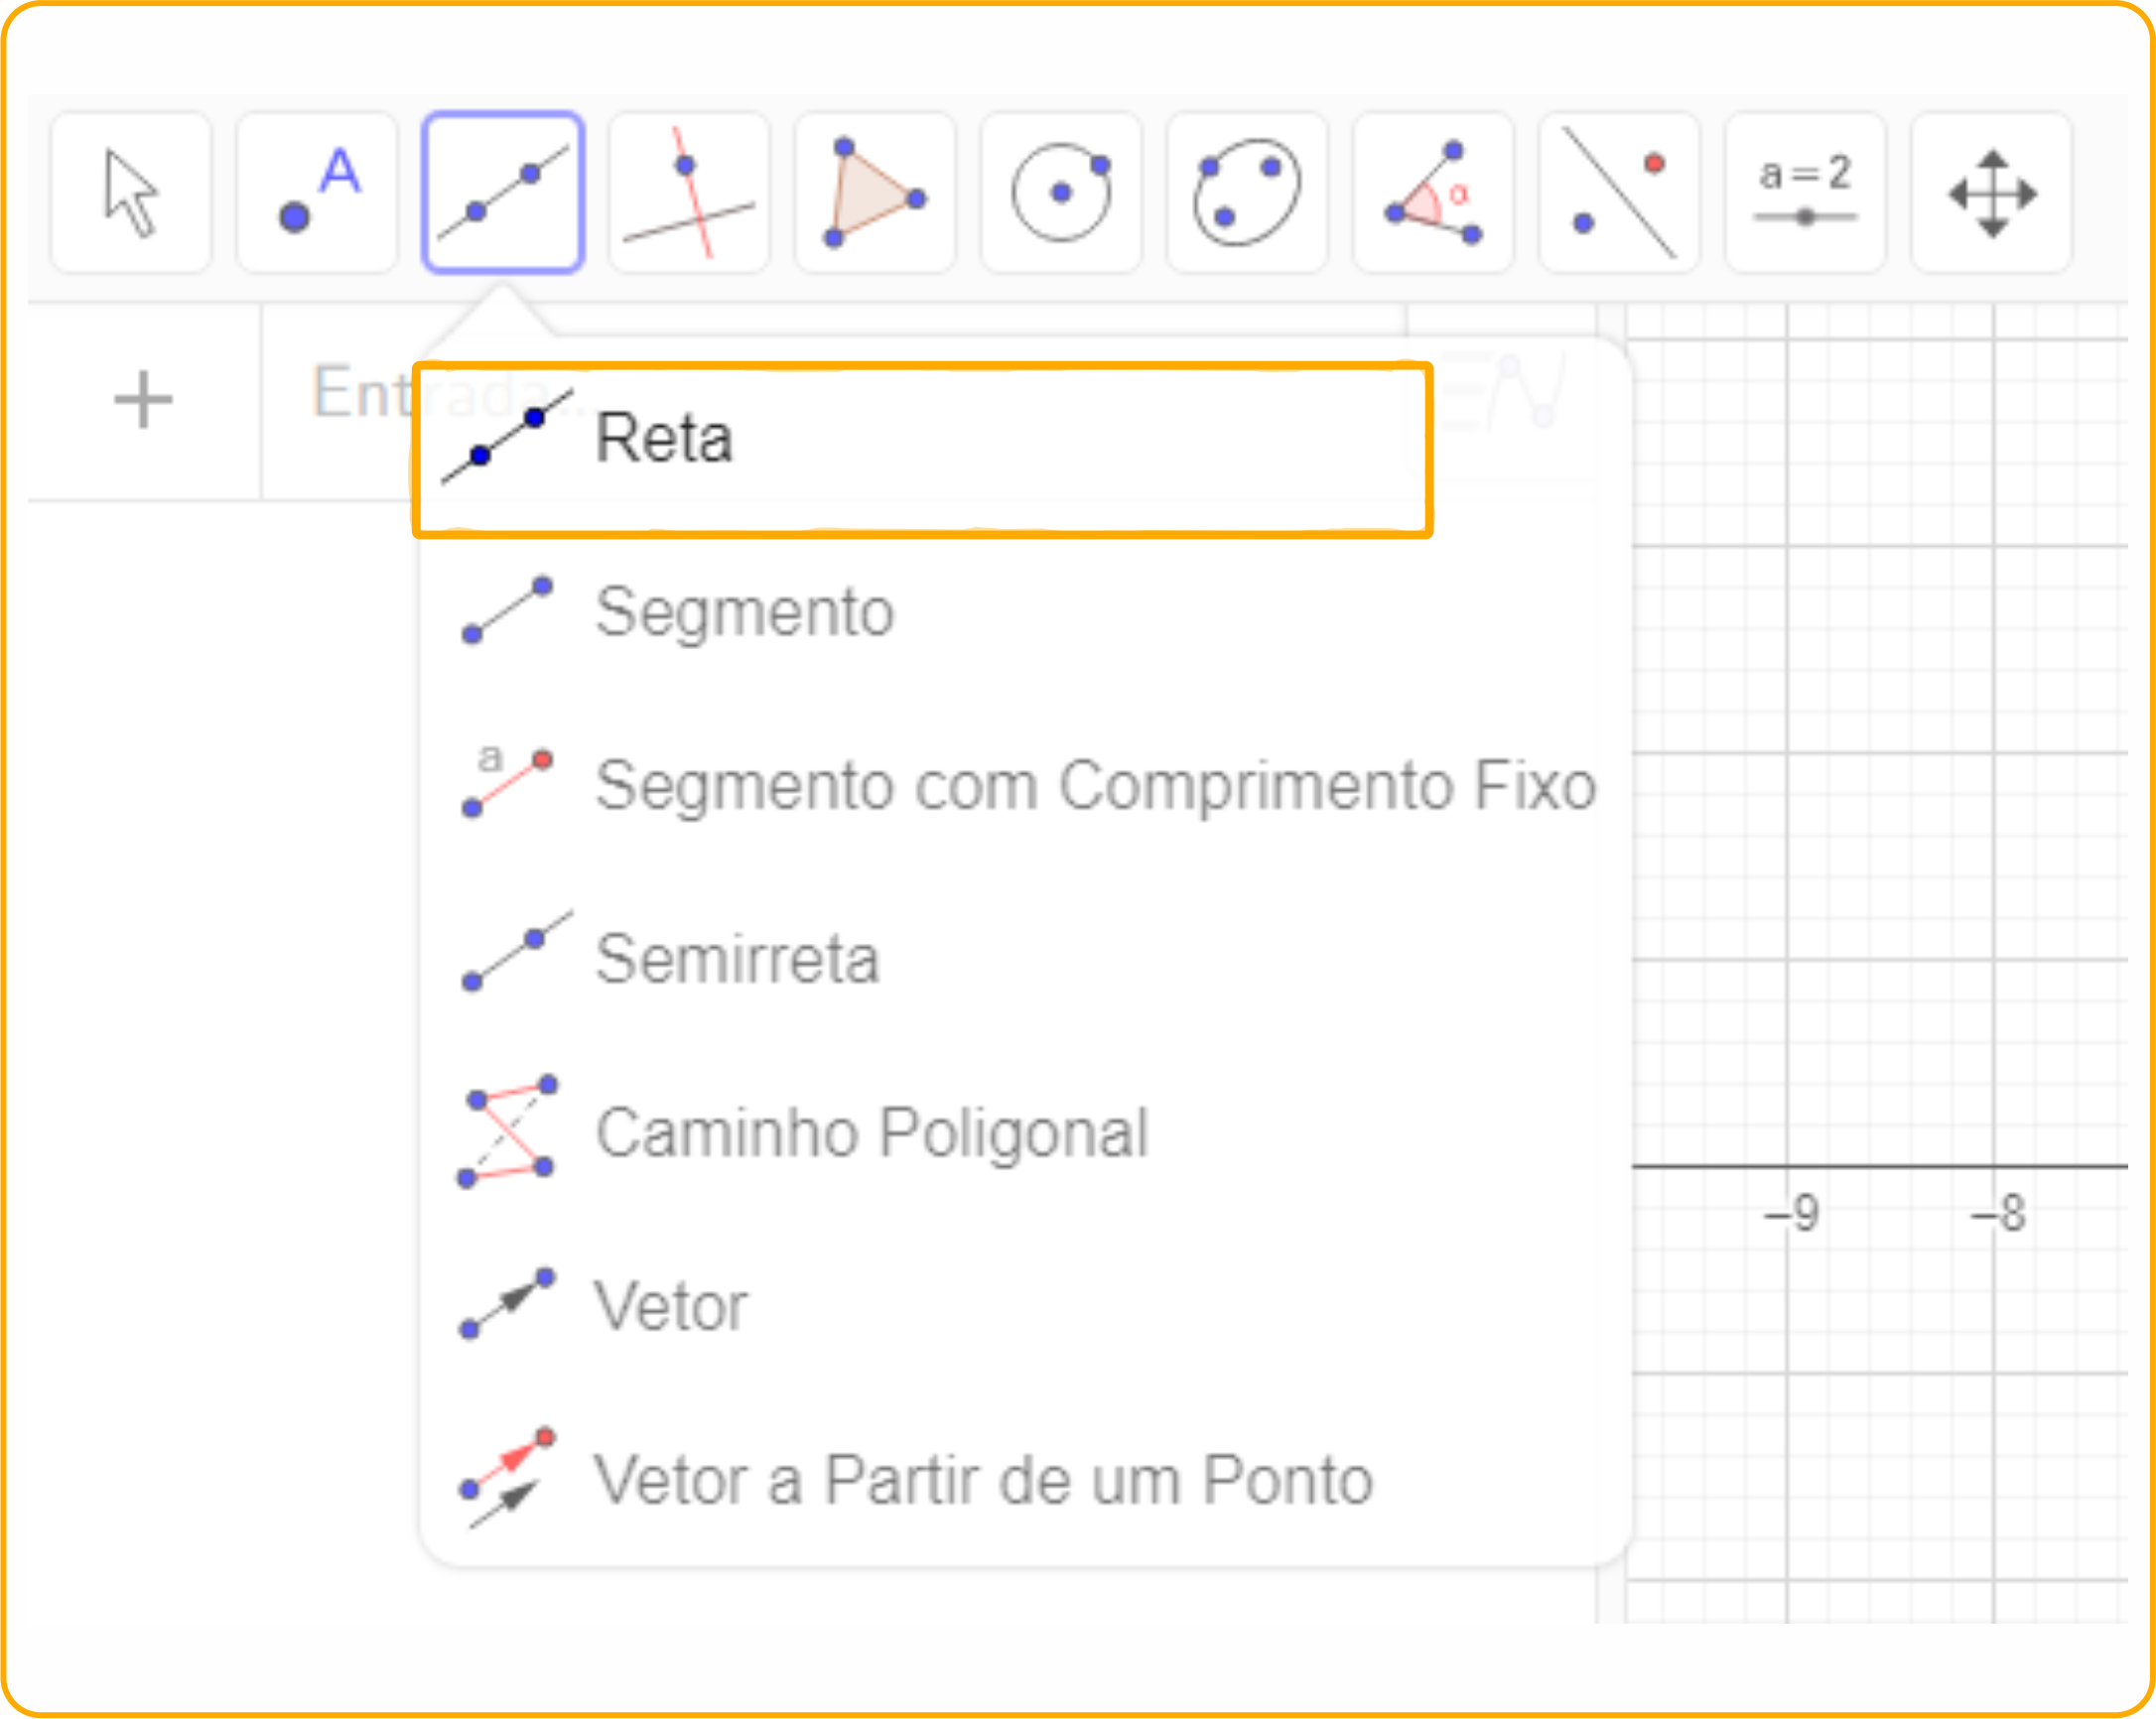
\includegraphics[height=8cm]{Figuras/T01_Elemento02.png}
    \caption{Atividade III - Etapa \ref{Atividade03_Etapa01}}
    \label{Atividade03_Etapa01_Imagem}
\end{figure}

\item Construa a reta $r$ que passe pelos pontos $A$ e $R$, sendo a coordenada do ponto $A (-2,0)$ e do ponto $R (4,1)$. \label{Atividade03_Etapa02}
\begin{figure}[H]
    \centering
    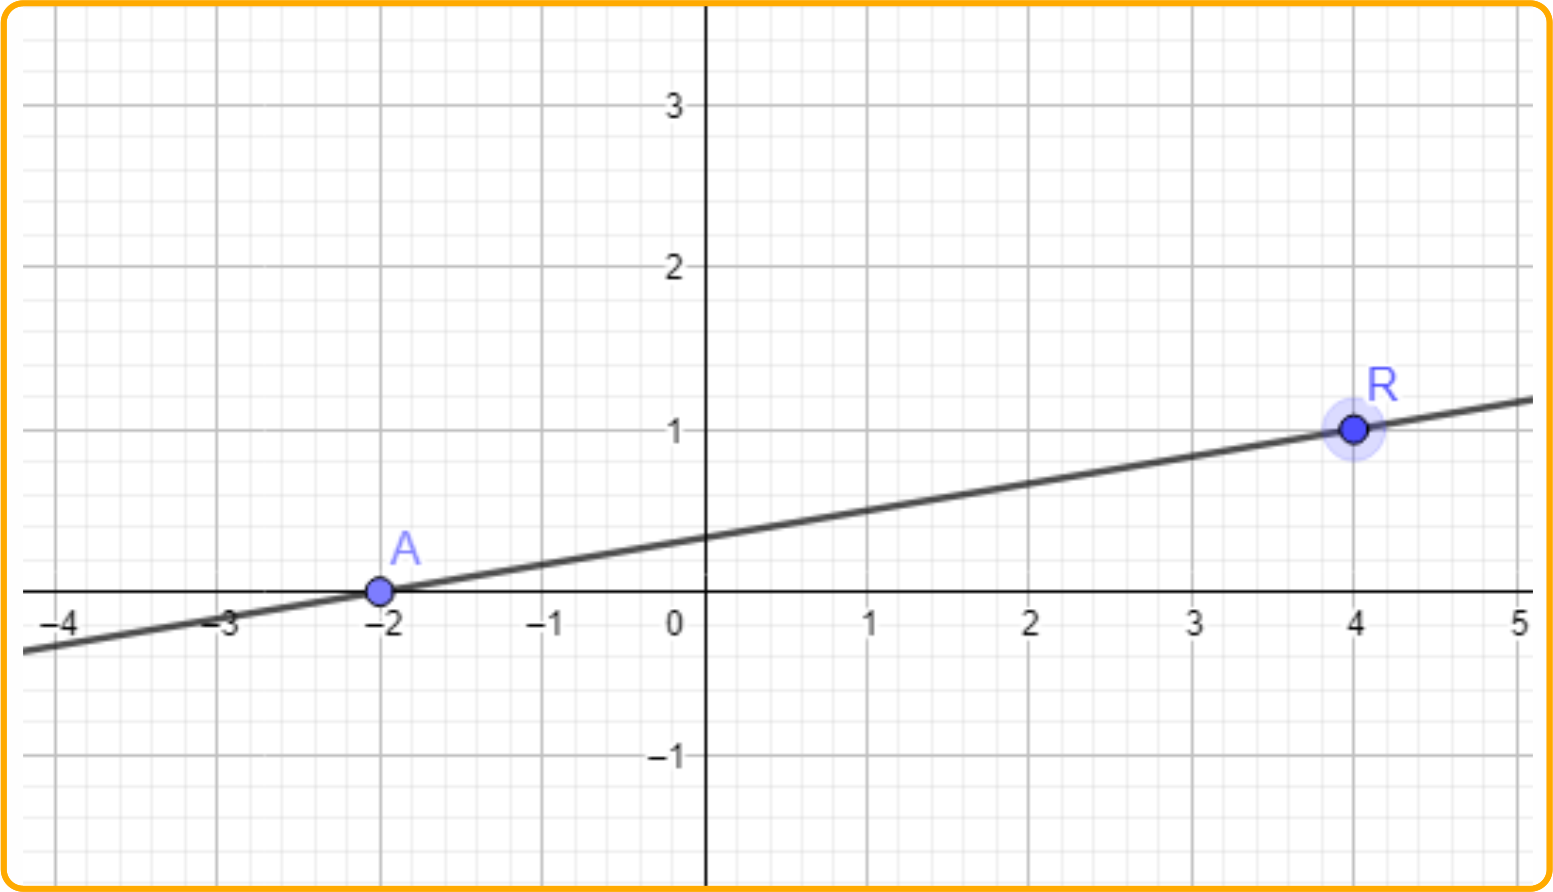
\includegraphics[height=7cm]{Figuras/T01_Atividade02_Fig01.png}
    \caption{Atividade III - Etapa \ref{Atividade03_Etapa02}}
    \label{Atividade03_Etapa02_Imagem}
\end{figure}

\item Selecione o ícone em destaque e clique na opção {\it ponto} \label{Atividade03_Etapa03}
\begin{figure}[H]
    \centering
    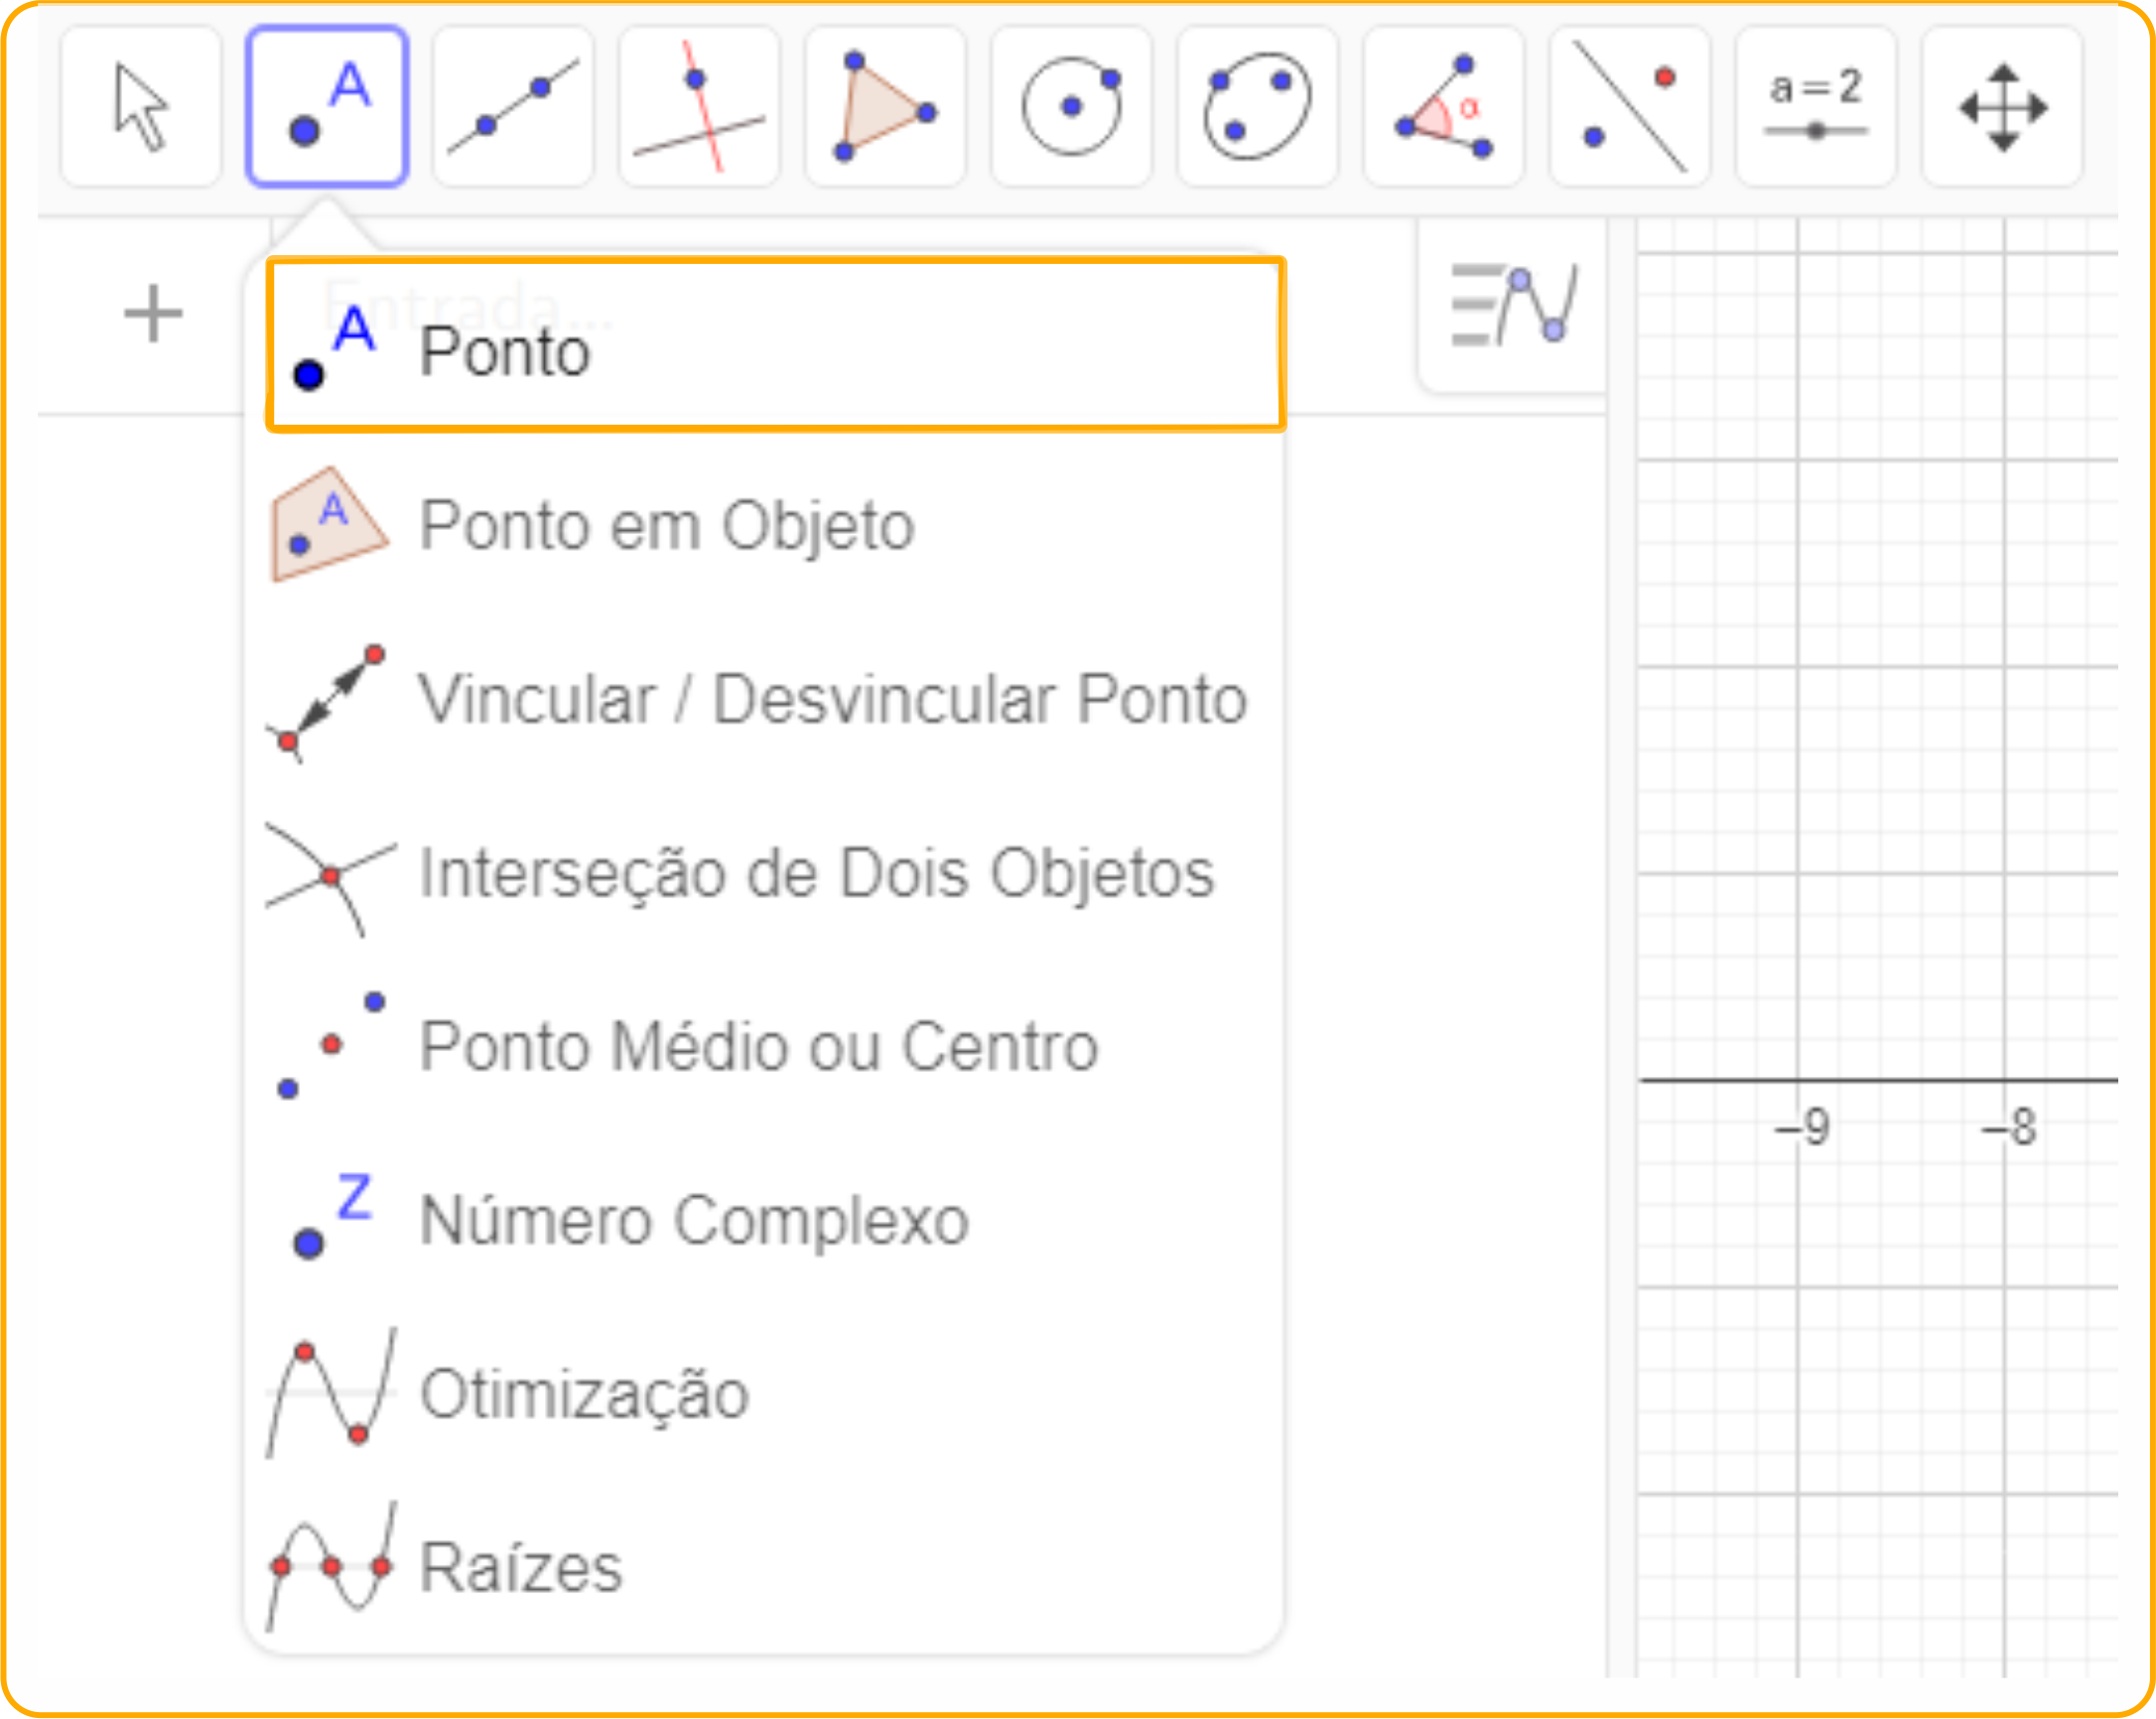
\includegraphics[height=8cm]{Figuras/T01_Elemento01.png}
    \caption{Atividade III - Etapa \ref{Atividade03_Etapa03}}
    \label{Atividade03_Etapa03_Imagem}
\end{figure}

\item Construa o ponto ${\color{blue}{P}}$ de coordenada $(-2,2)$. \label{Atividade03_Etapa04}
\begin{figure}[H]
    \centering
    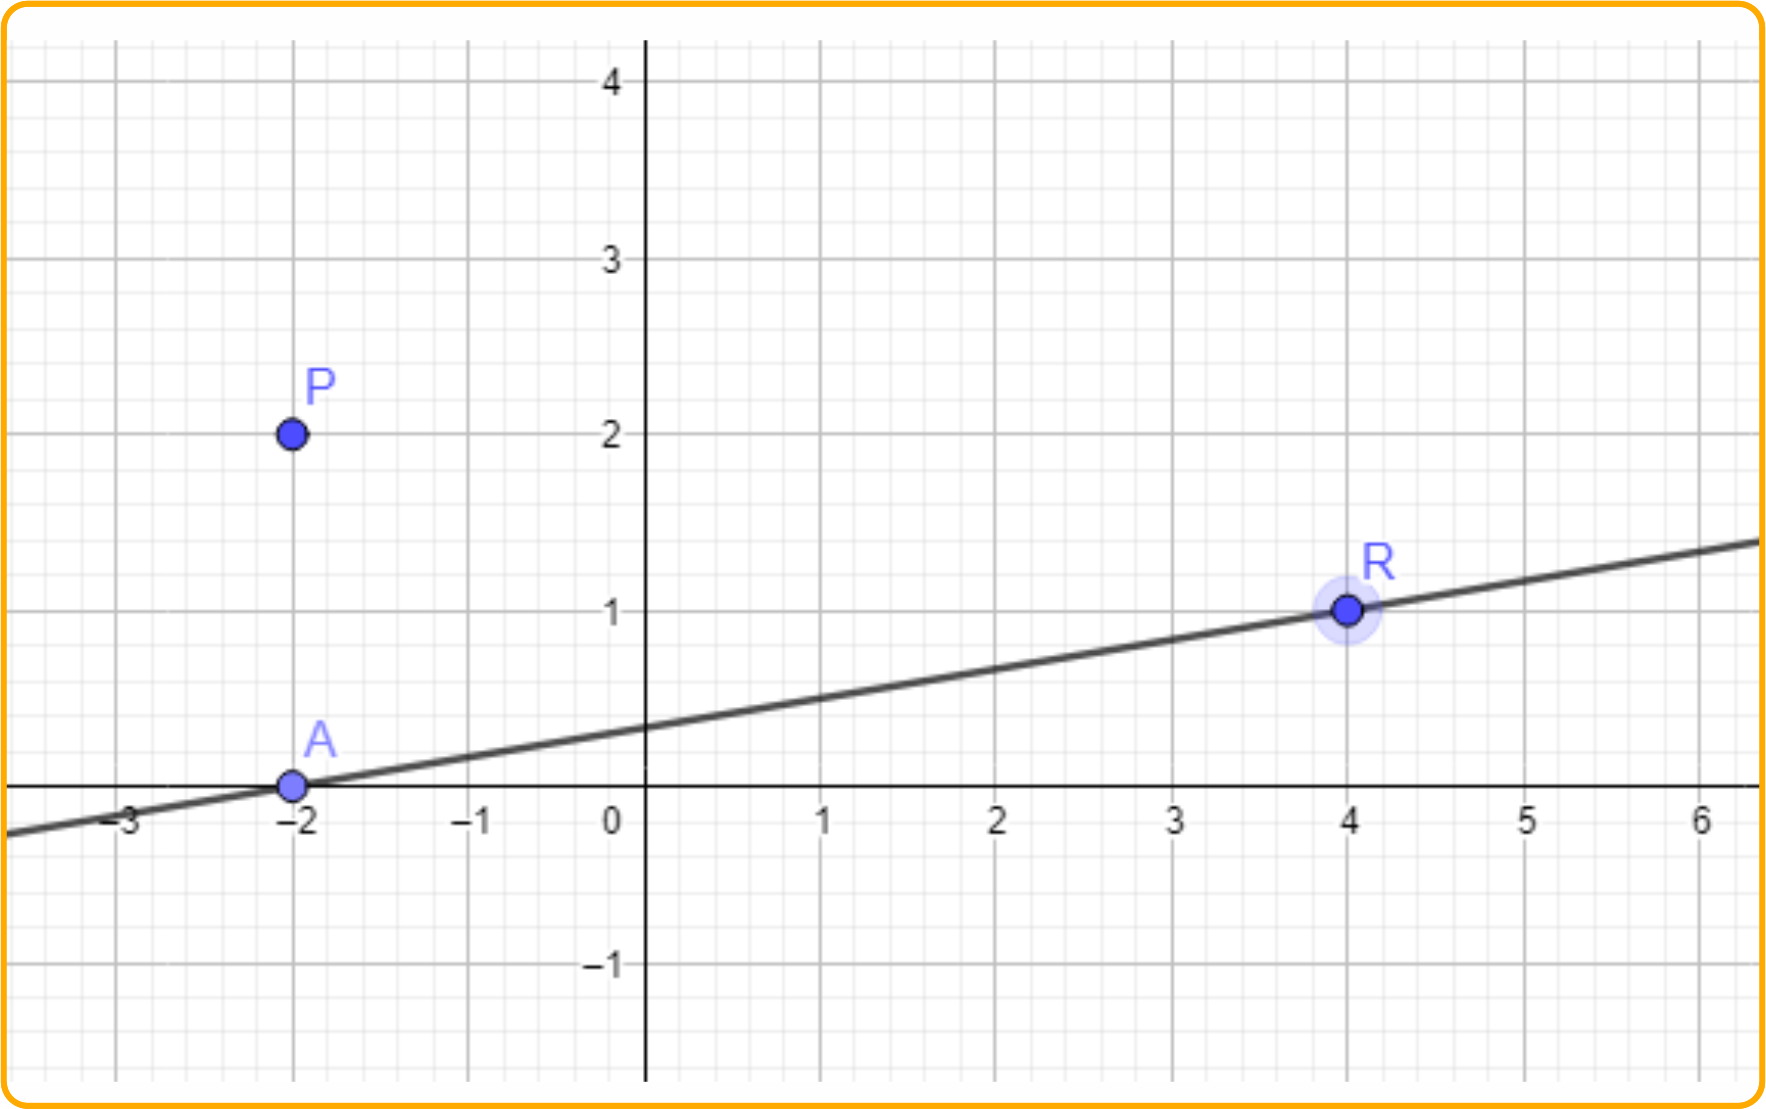
\includegraphics[height=8cm]{Figuras/T01_Atividade02_Fig02.png}
    \caption{Atividade III - Etapa \ref{Atividade03_Etapa04}}
    \label{Atividade03_Etapa04_Imagem}
\end{figure}

\item Selecione o ícone em destaque e clique na opção {\it círculo: centro \& raio}. \label{Atividade03_Etapa05}
\begin{figure}[H]
    \centering
    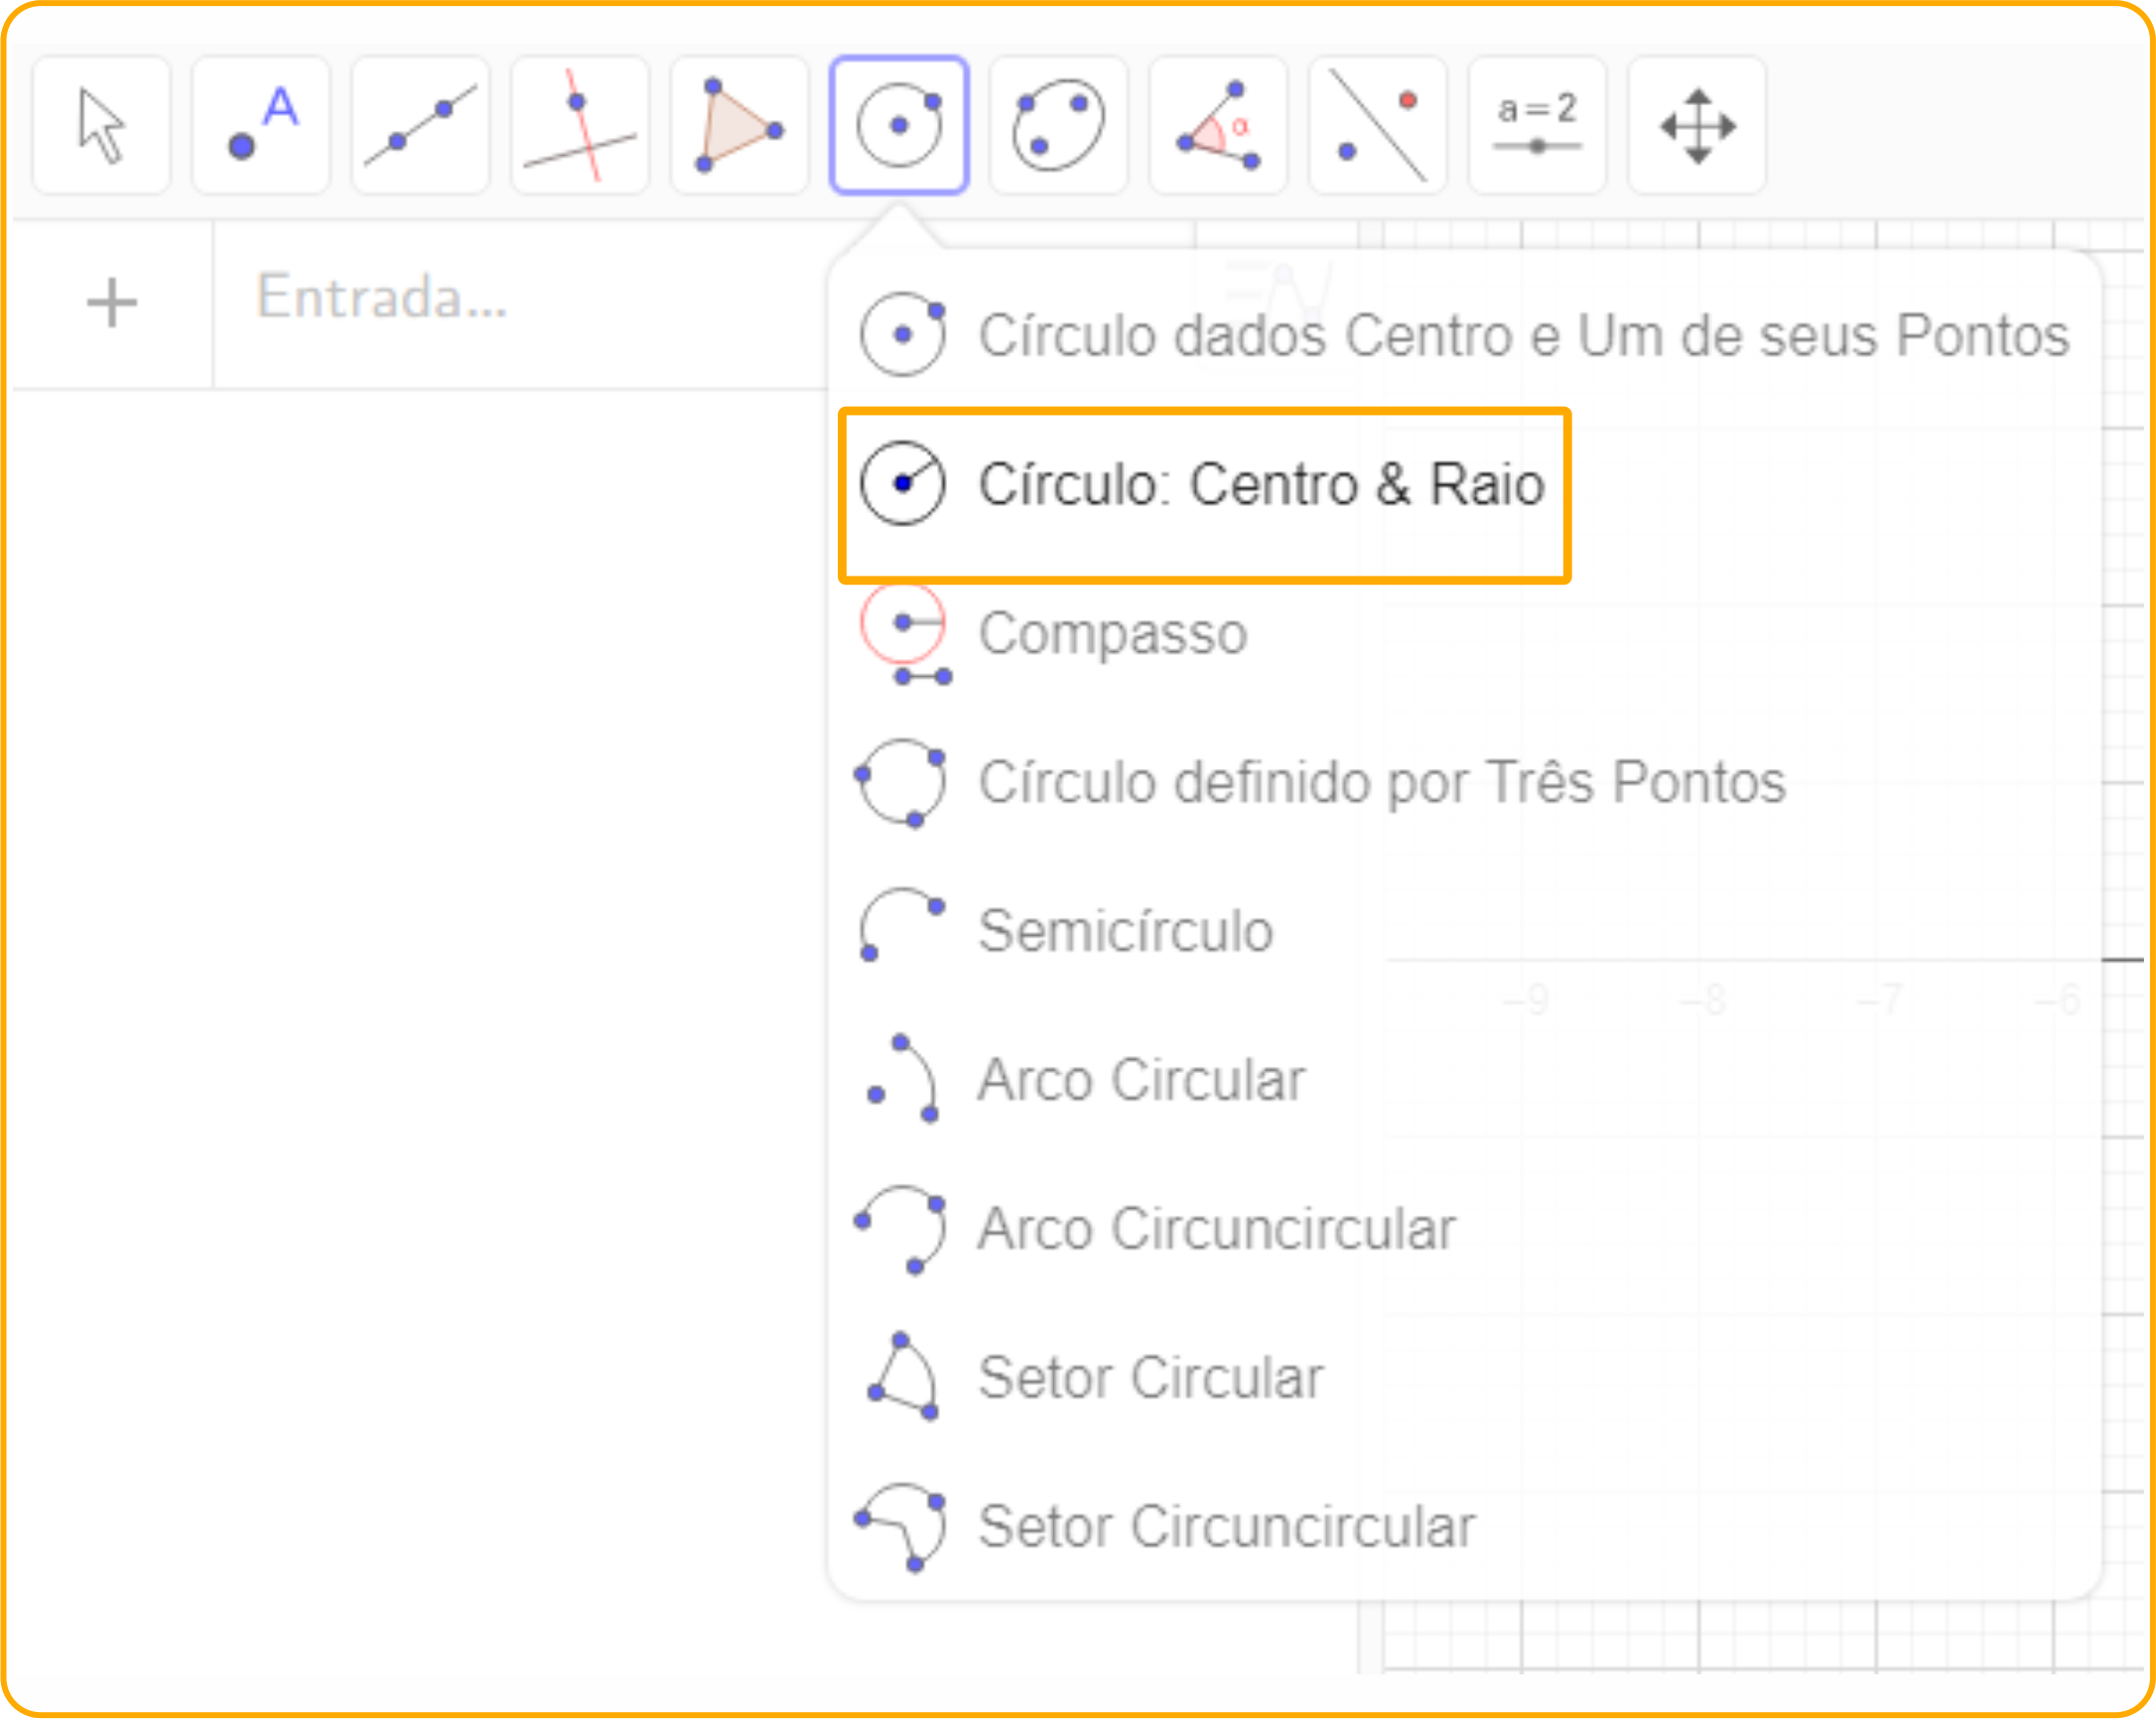
\includegraphics[height=8cm]{Figuras/T01_Elemento07.png}
    \caption{Atividade III - Etapa \ref{Atividade03_Etapa05}}
    \label{Atividade03_Etapa05_Imagem}
\end{figure}

\item Selecione o ponto ${\color{blue}{P}}$ e trace a circunferência ${\color{red}{c}}$ de raio $3$. \label{Atividade03_Etapa06}
\begin{figure}[H]
    \centering
    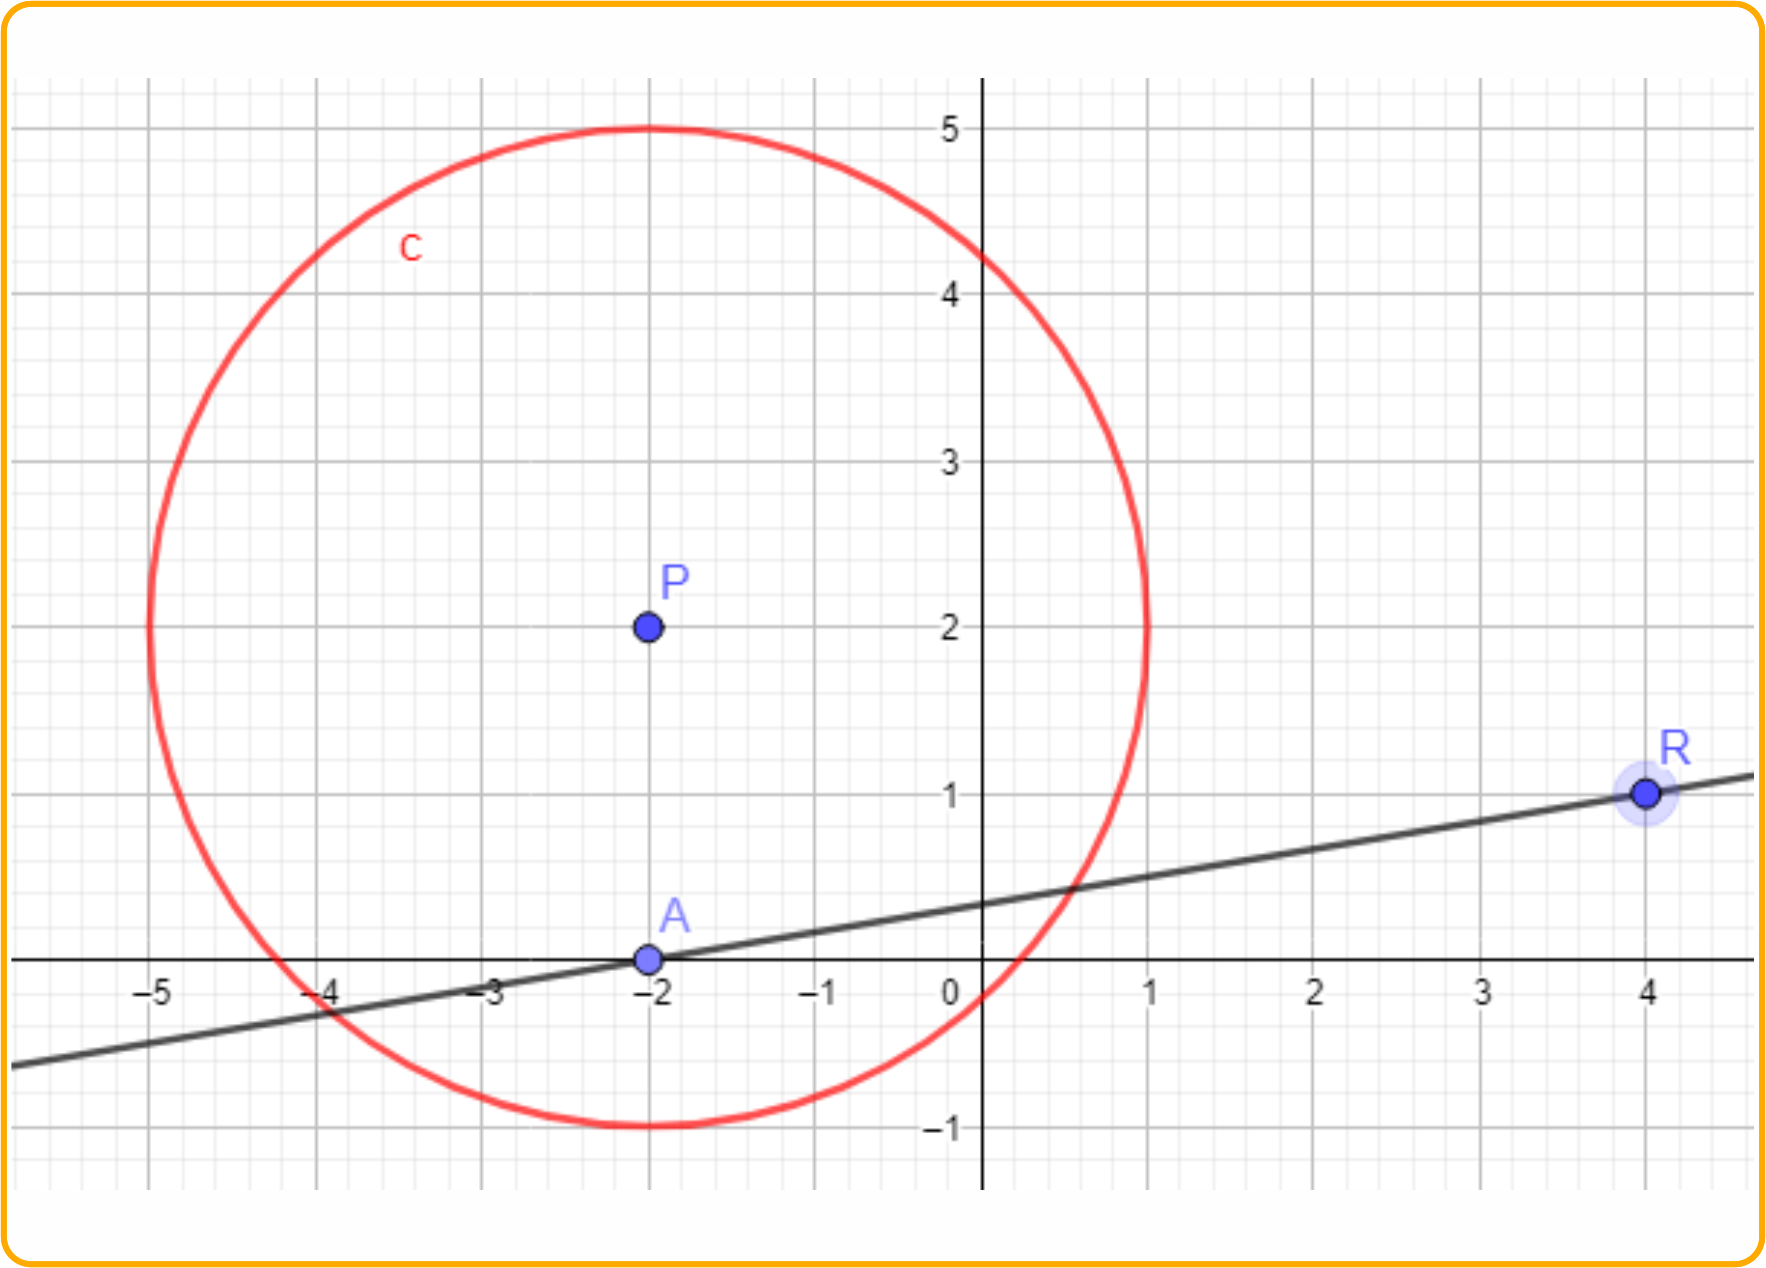
\includegraphics[height=8cm]{Figuras/T01_Atividade02_Fig03.png}
    \caption{Atividade III - Etapa \ref{Atividade03_Etapa06}}
    \label{Atividade03_Etapa06_Imagem}
\end{figure}

\item Selecione o ícone em destaque e clique na opção {\it interseção de dois objetos}. \label{Atividade03_Etapa07}
\begin{figure}[H]
    \centering
    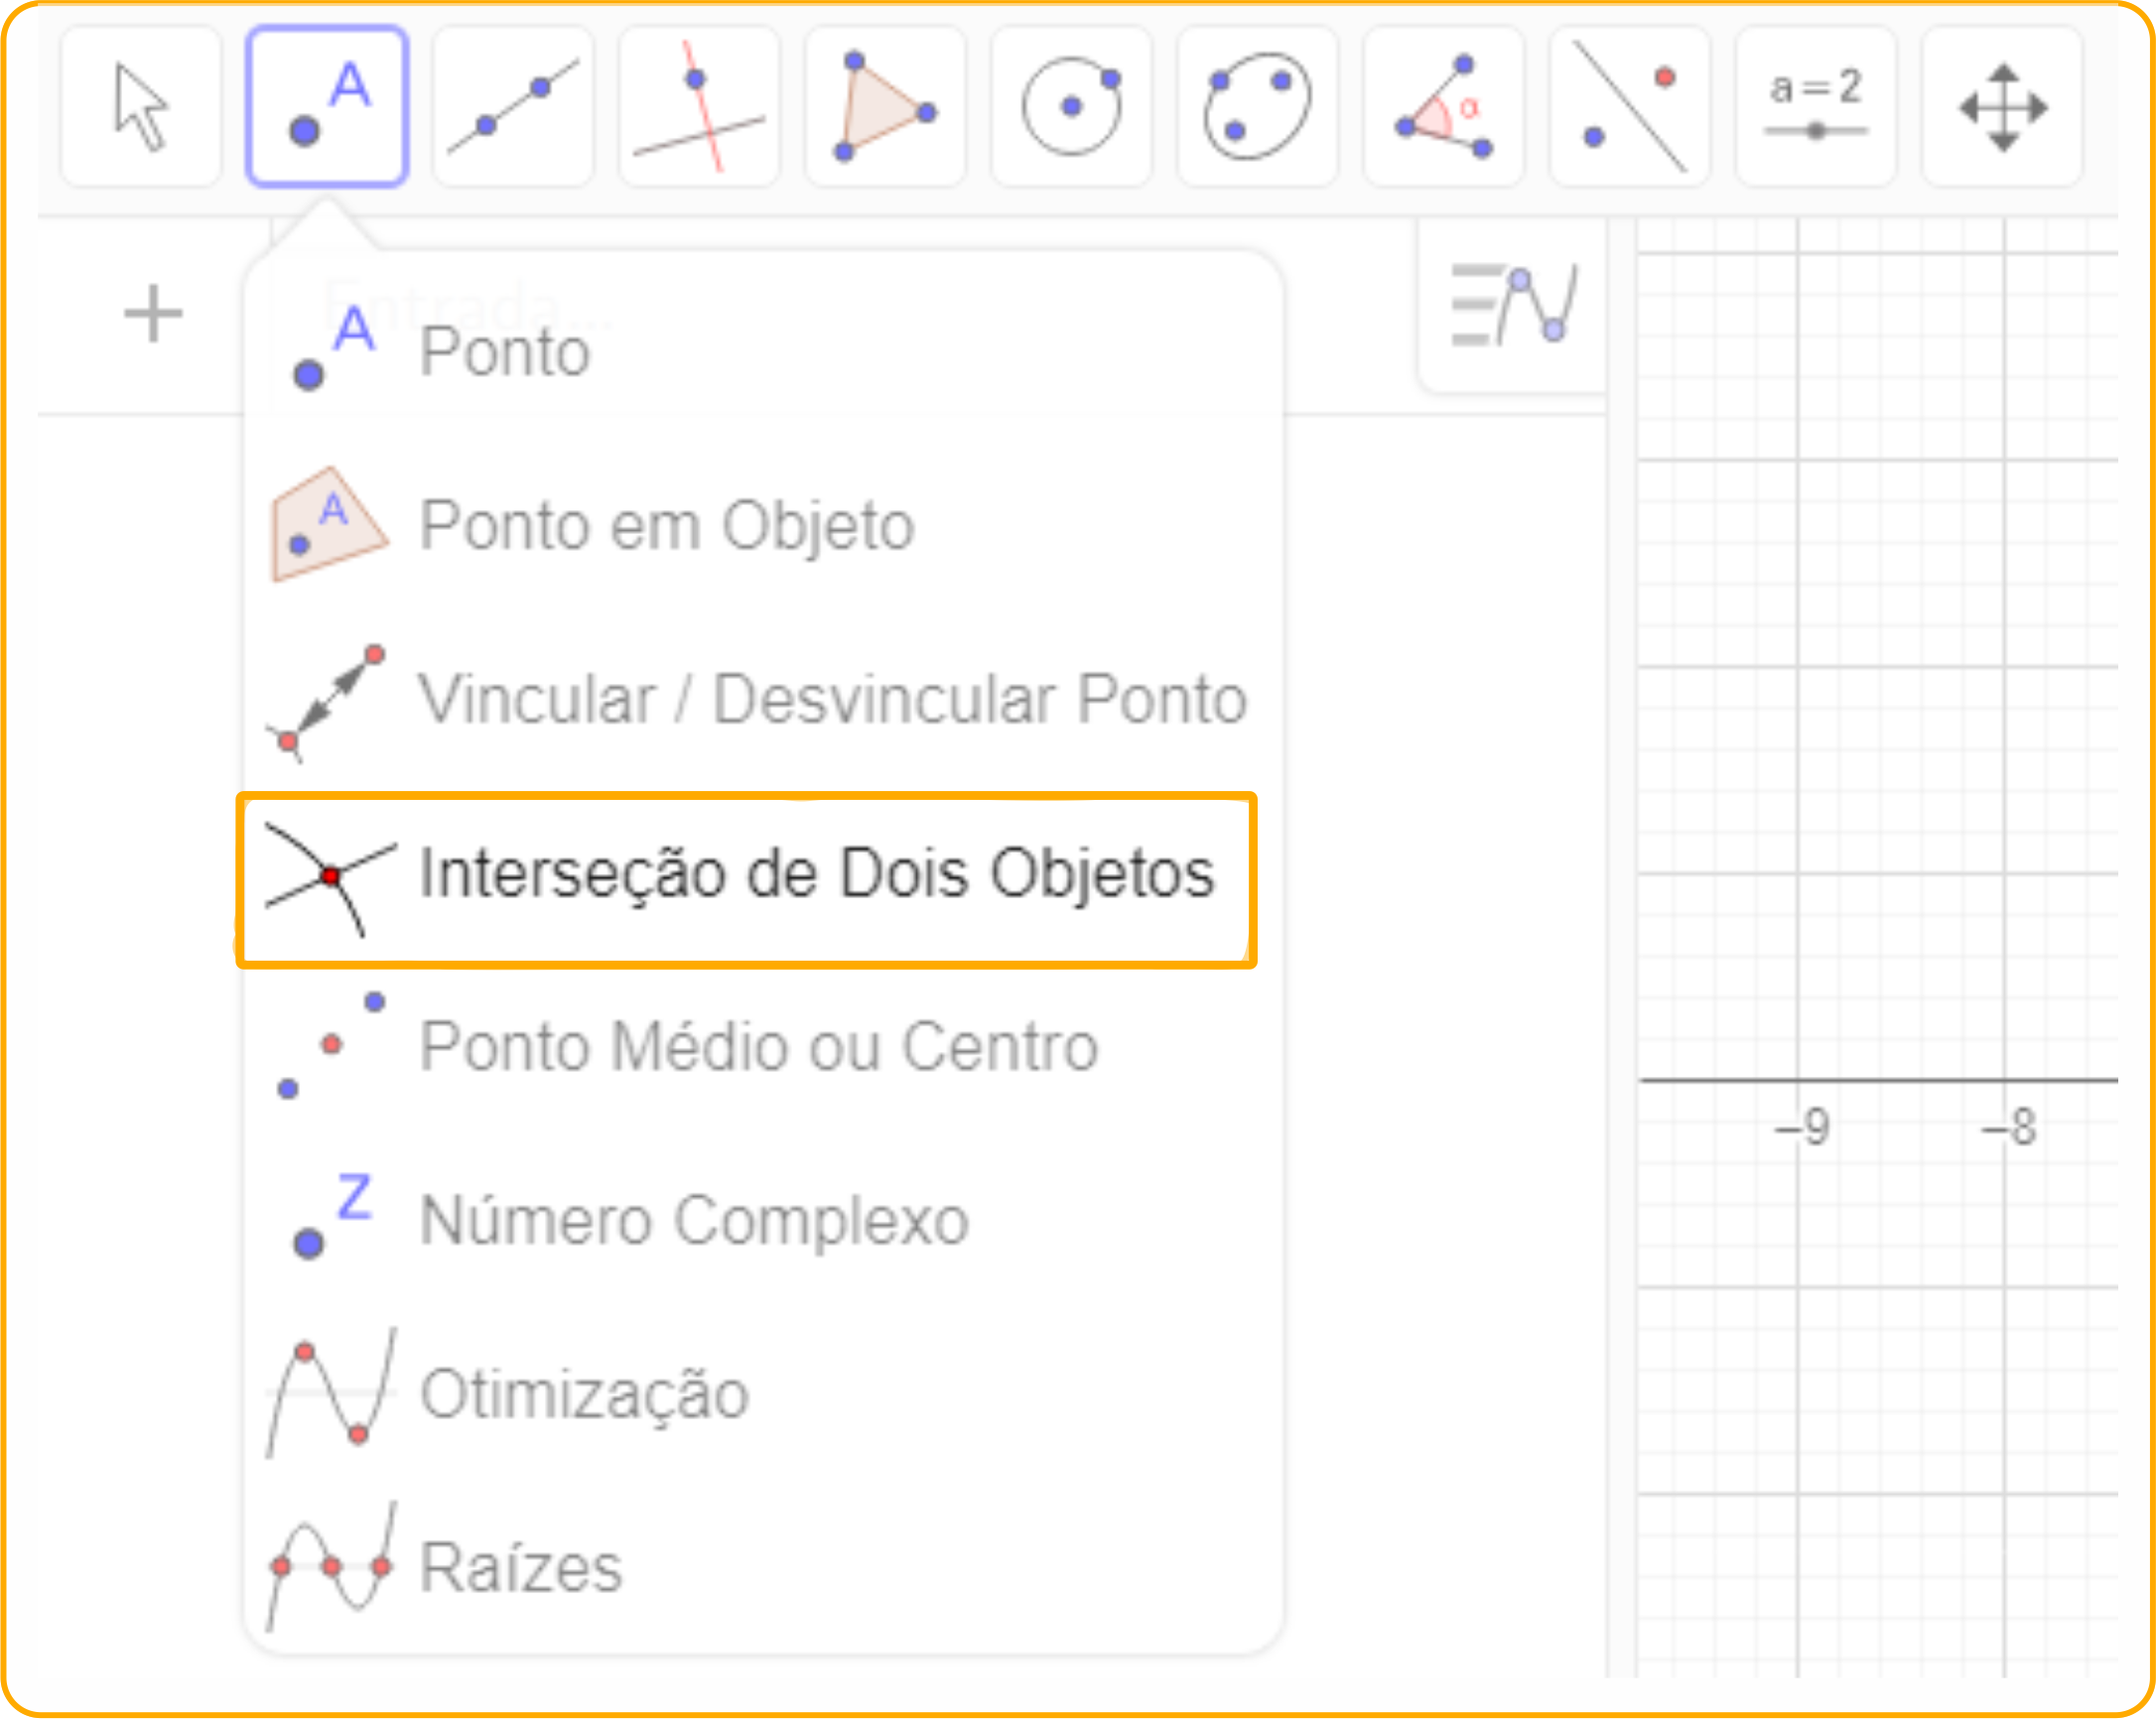
\includegraphics[height=8cm]{Figuras/T01_Elemento05.png}
    \caption{Atividade III - Etapa \ref{Atividade03_Etapa07}}
    \label{Atividade03_Etapa07_Imagem}
\end{figure}

\item Construa os pontos $E$ e $F$ nas interseções da circunferência ${\color{red}{c}}$ com a reta $r$. \label{Atividade03_Etapa08}
\begin{figure}[H]
    \centering
    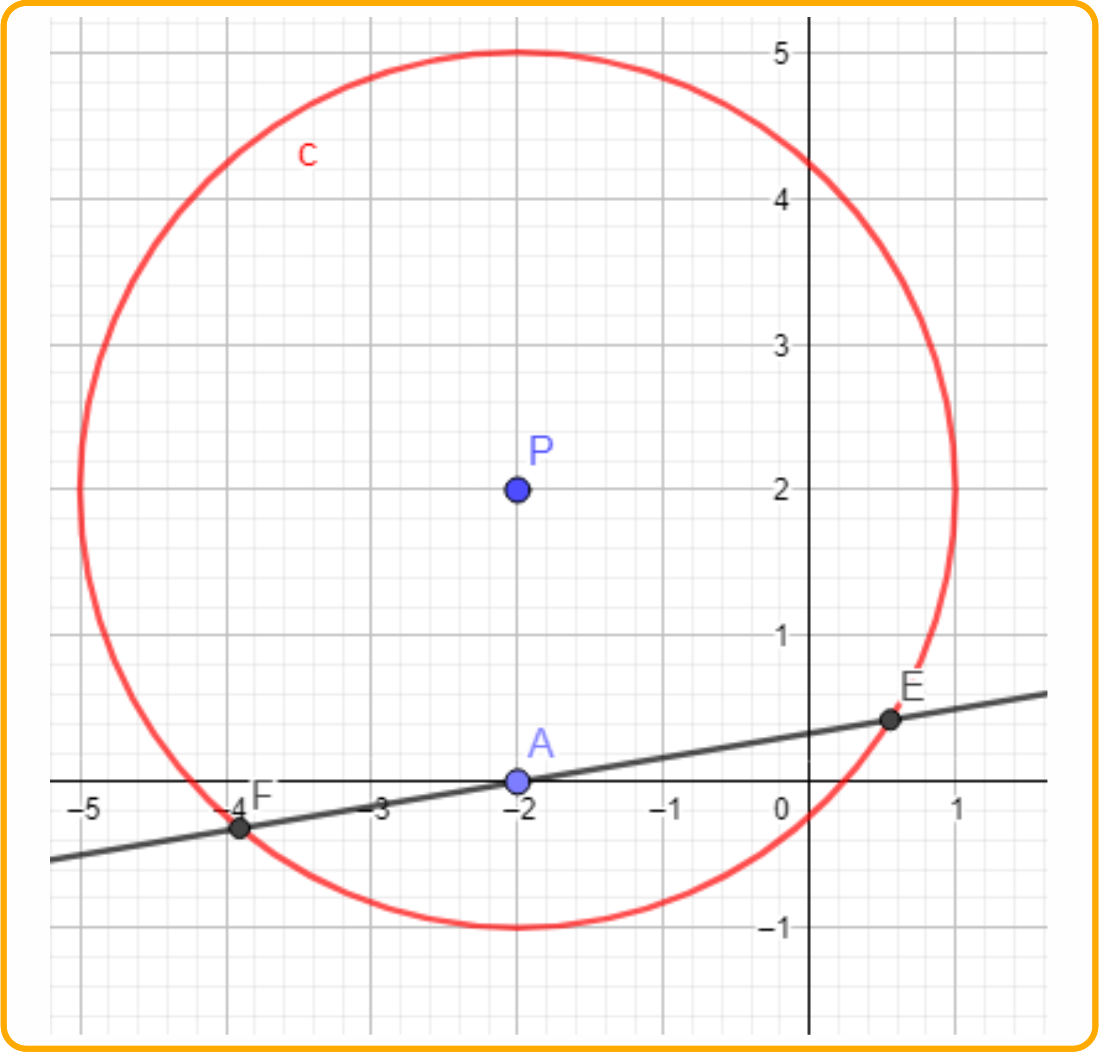
\includegraphics[height=6cm]{Figuras/T01_Atividade03_Fig01.png}
    \caption{Atividade III - Etapa \ref{Atividade03_Etapa08}}
    \label{Atividade03_Etapa08_Imagem}
\end{figure}

\item Selecione o ícone em destaque e clique na opção {\it compasso}. \label{Atividade03_Etapa09}
\begin{figure}[H]
    \centering
    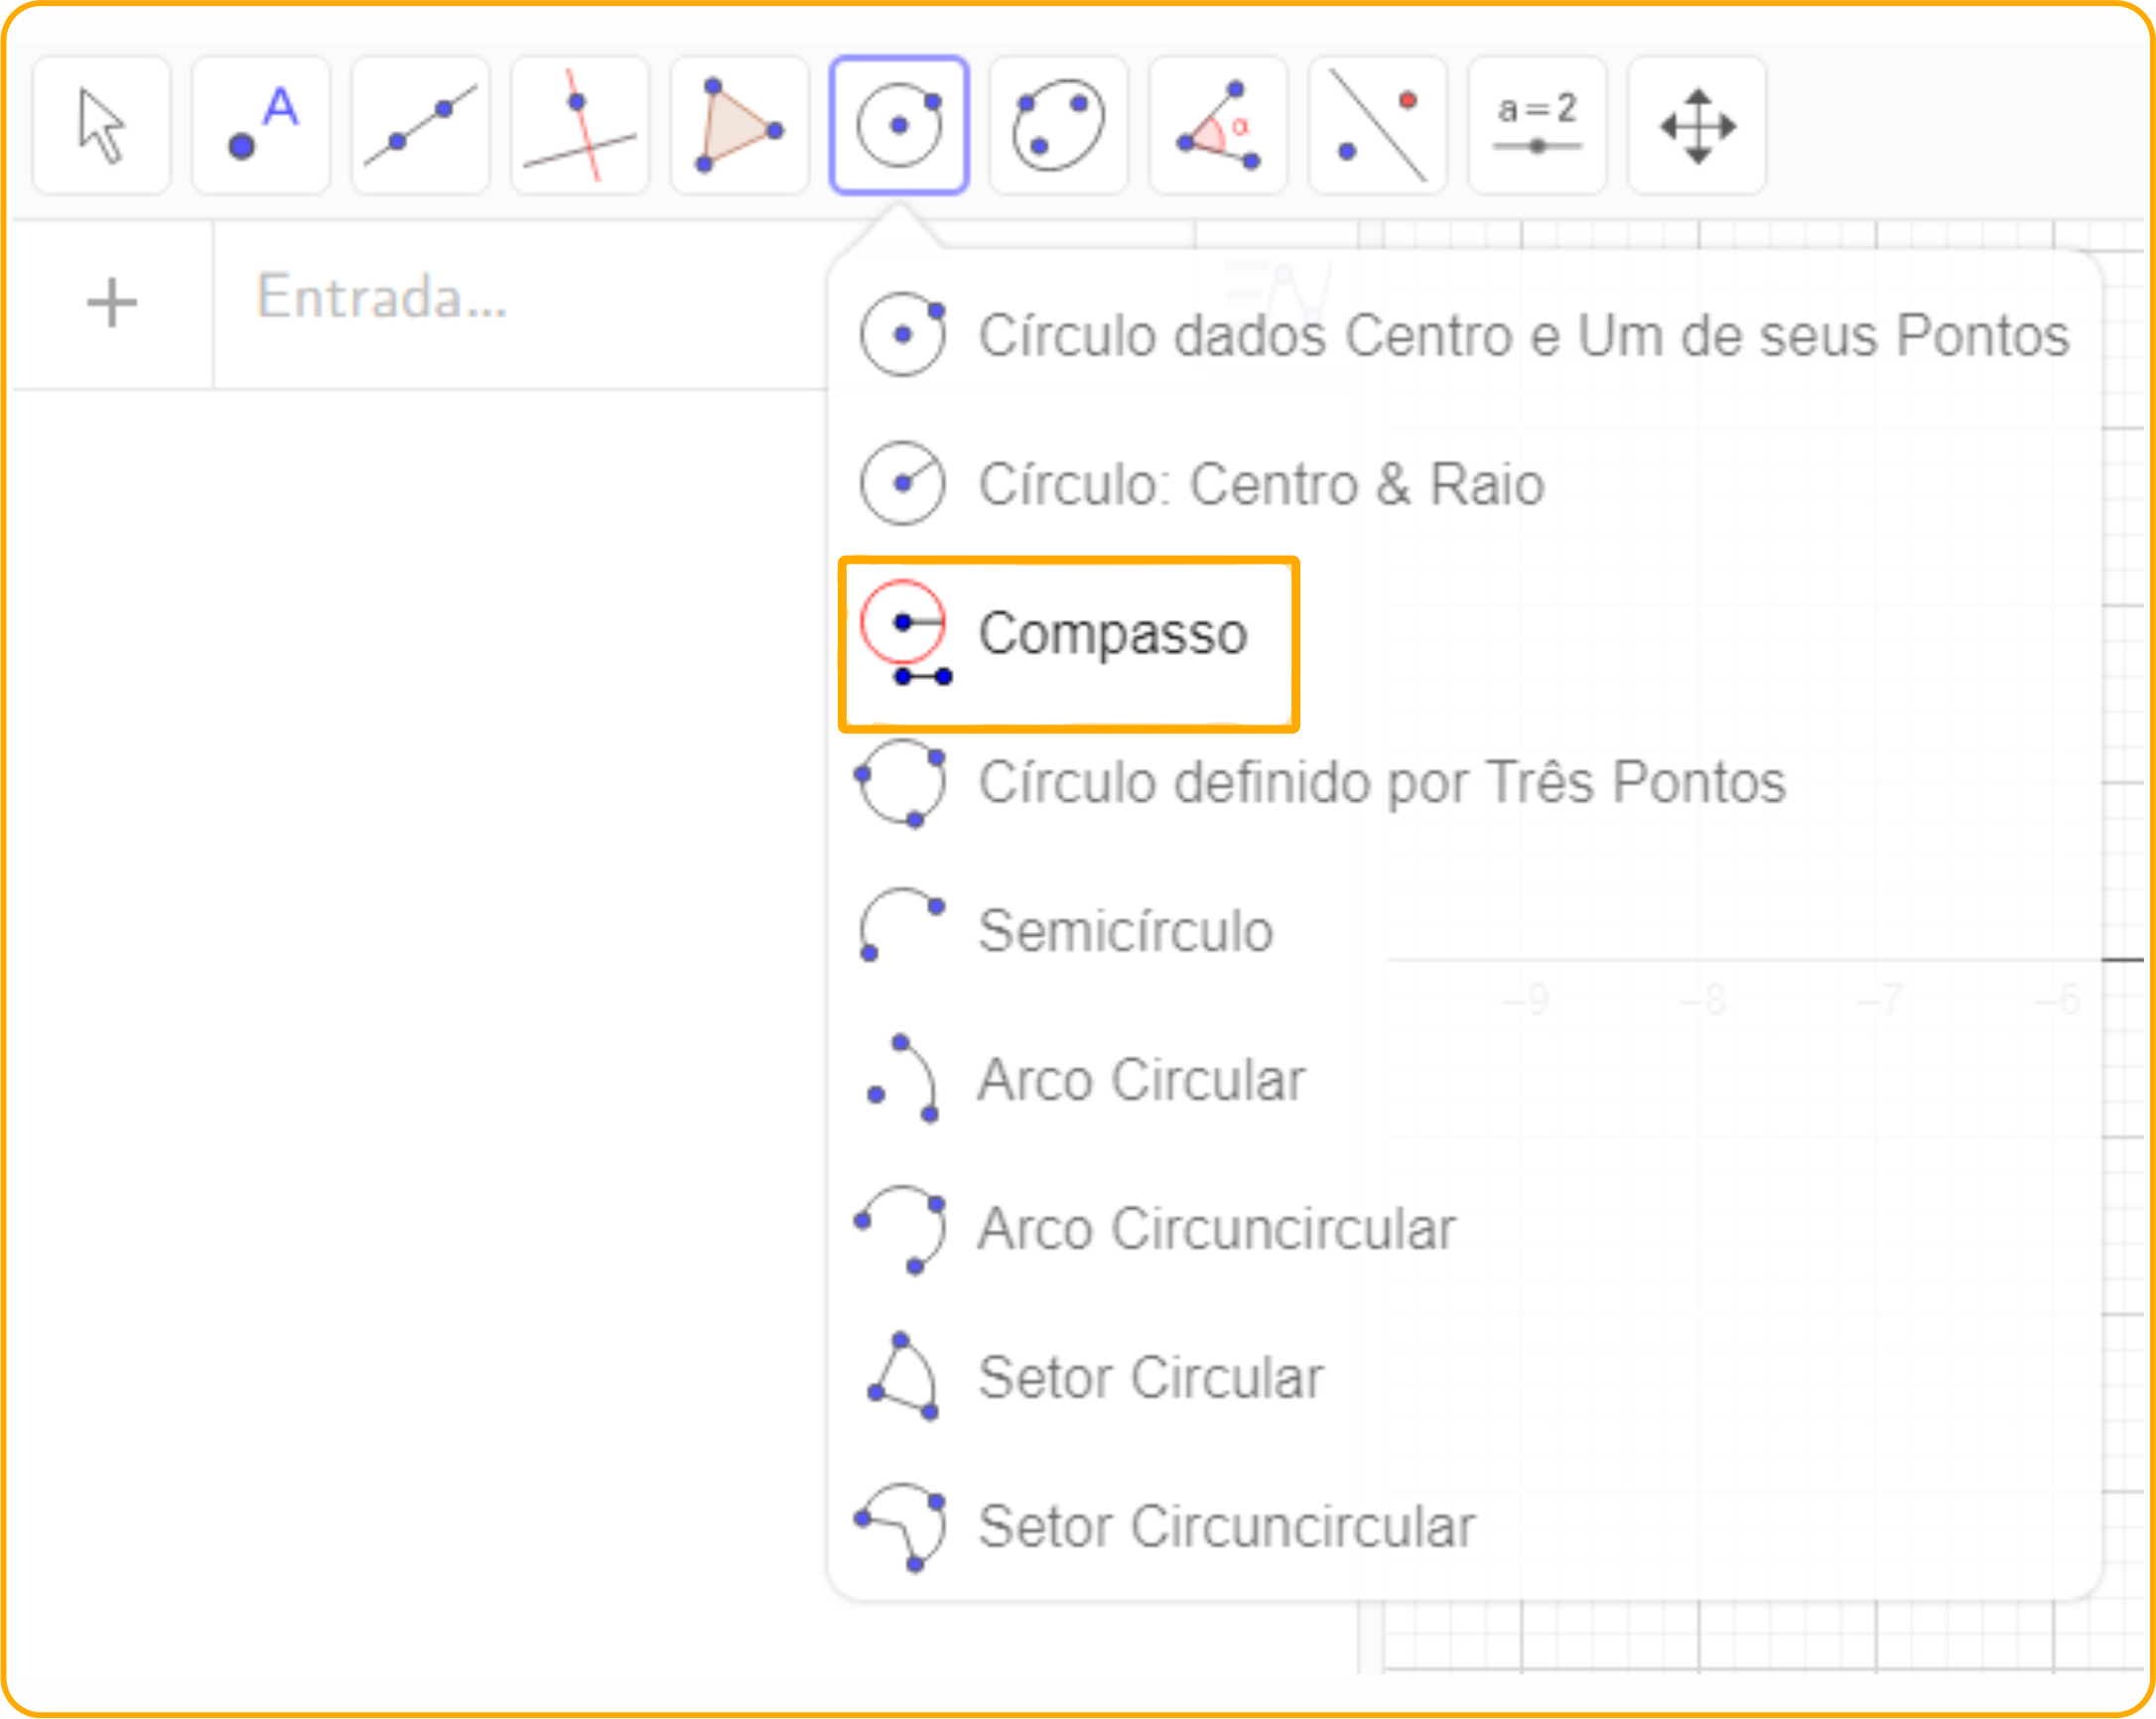
\includegraphics[height=8cm]{Figuras/T01_Elemento04.png}
    \caption{Atividade III - Etapa \ref{Atividade03_Etapa09}}
    \label{Atividade03_Etapa09_Imagem}
\end{figure}

\item Construa uma circunferência ${\color{green}{f}}$ com centro no ponto $F$ e com raio de mesma medida que o segmento $\overline{PF}$. \label{Atividade03_Etapa10}
\begin{figure}[H]
    \centering
    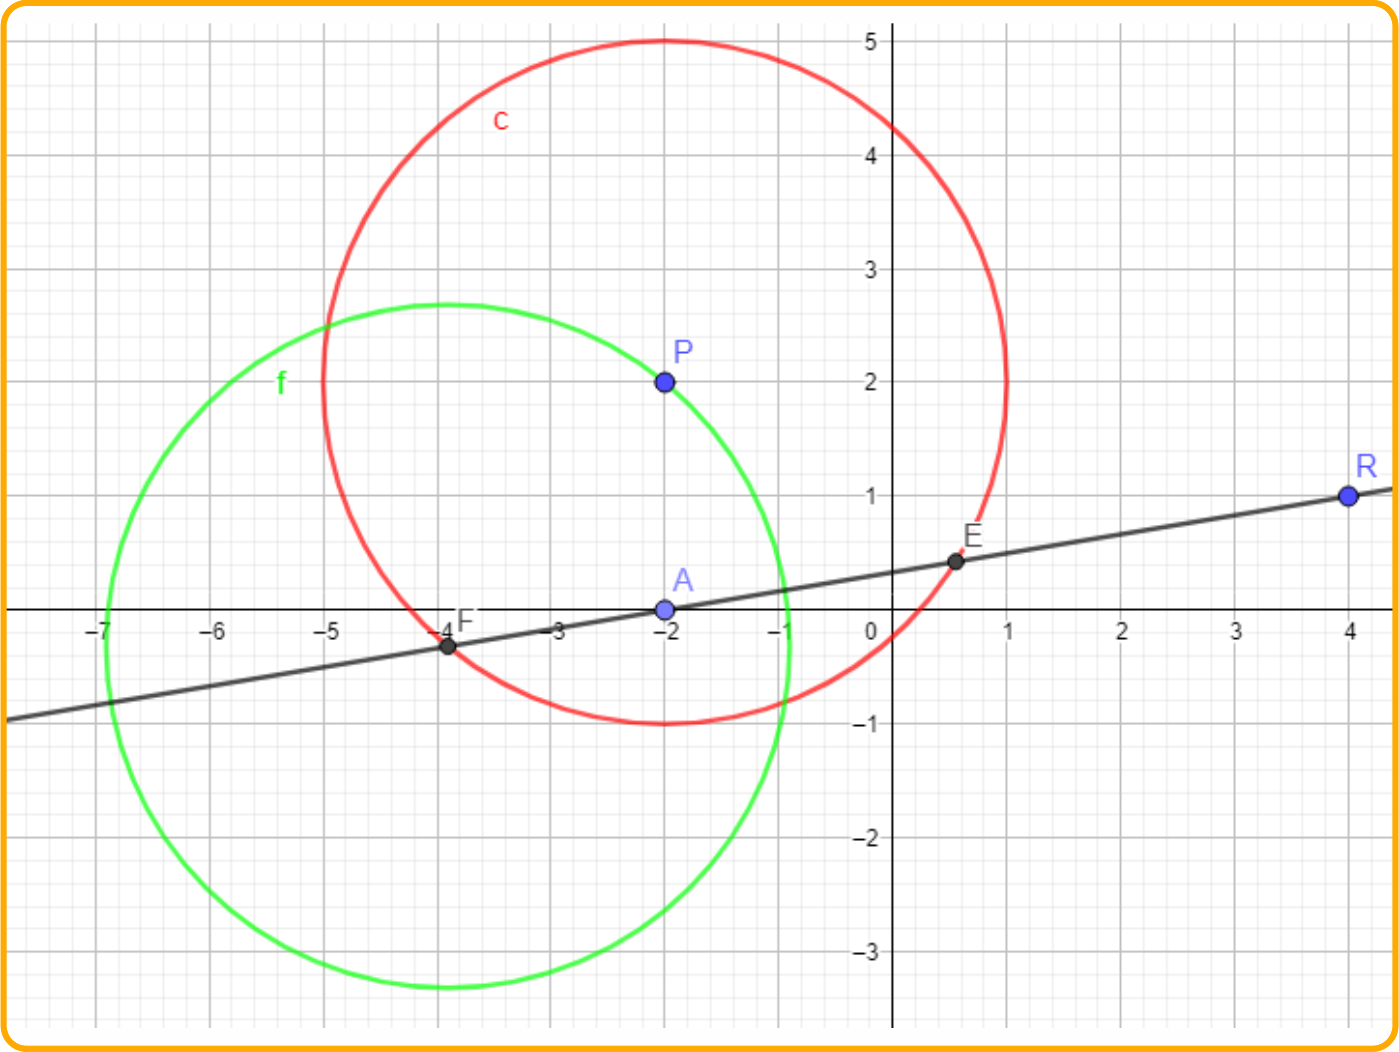
\includegraphics[height=8cm]{Figuras/T01_Atividade03_Fig02.png}
    \caption{Atividade III - Etapa \ref{Atividade03_Etapa10}}
    \label{Atividade03_Etapa10_Imagem}
\end{figure}

\item Repita a Etapa \ref{Atividade03_Etapa09} e construa uma circunferência ${\color{orange}{g}}$ com centro no ponto $E$ e com raio de mesma medida que o segmento $\overline{PE}$. \label{Atividade03_Etapa11}
\begin{figure}[H]
    \centering
    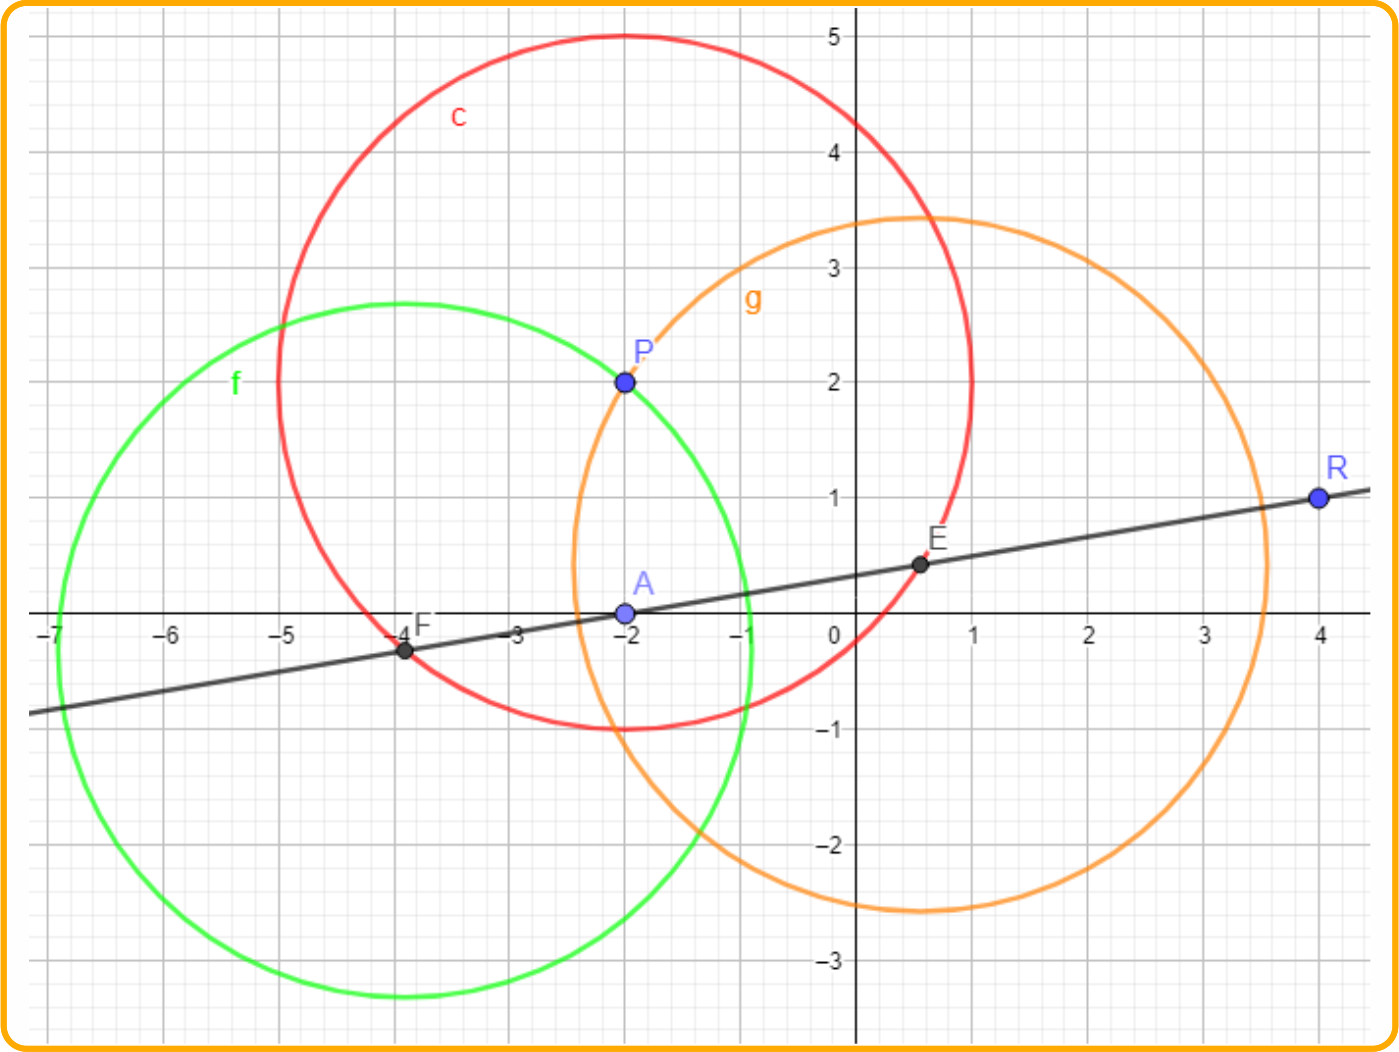
\includegraphics[height=8cm]{Figuras/T01_Atividade03_Fig03.png}
    \caption{Atividade III - Etapa \ref{Atividade03_Etapa11}}
    \label{Atividade03_Etapa11_Imagem}
\end{figure}

\item Repita a Etapa \ref{Atividade03_Etapa07} e marque o ponto $G$ na interseção das circunferências ${\color{ForestGreen}{f}}$ e ${\color{orange}{g}}$. \label{Atividade03_Etapa12}
\begin{figure}[H]
    \centering
    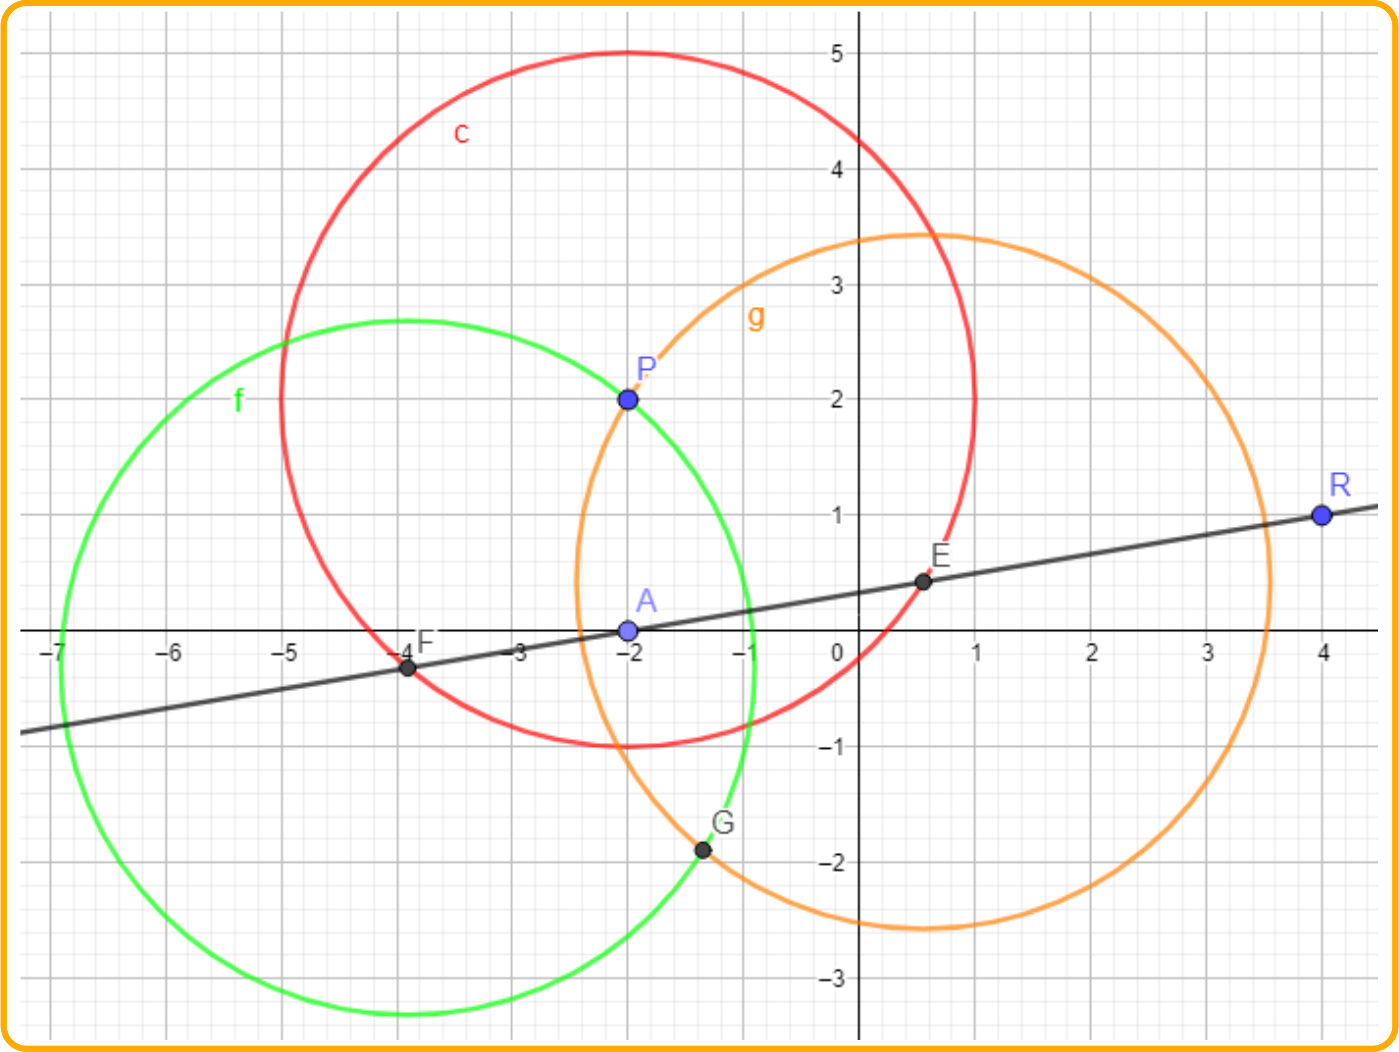
\includegraphics[height=8cm]{Figuras/T01_Atividade03_Fig04.png}
    \caption{Atividade III - Etapa \ref{Atividade03_Etapa12}}
    \label{Atividade03_Etapa12_Imagem}
\end{figure}

\item Repita a Etapa \ref{Atividade03_Etapa01} e construa a reta ${\color{magenta}{h}}$, que passa pelos pontos $P$ e $G$. \label{Atividade03_Etapa13}
\begin{figure}[H]
    \centering
    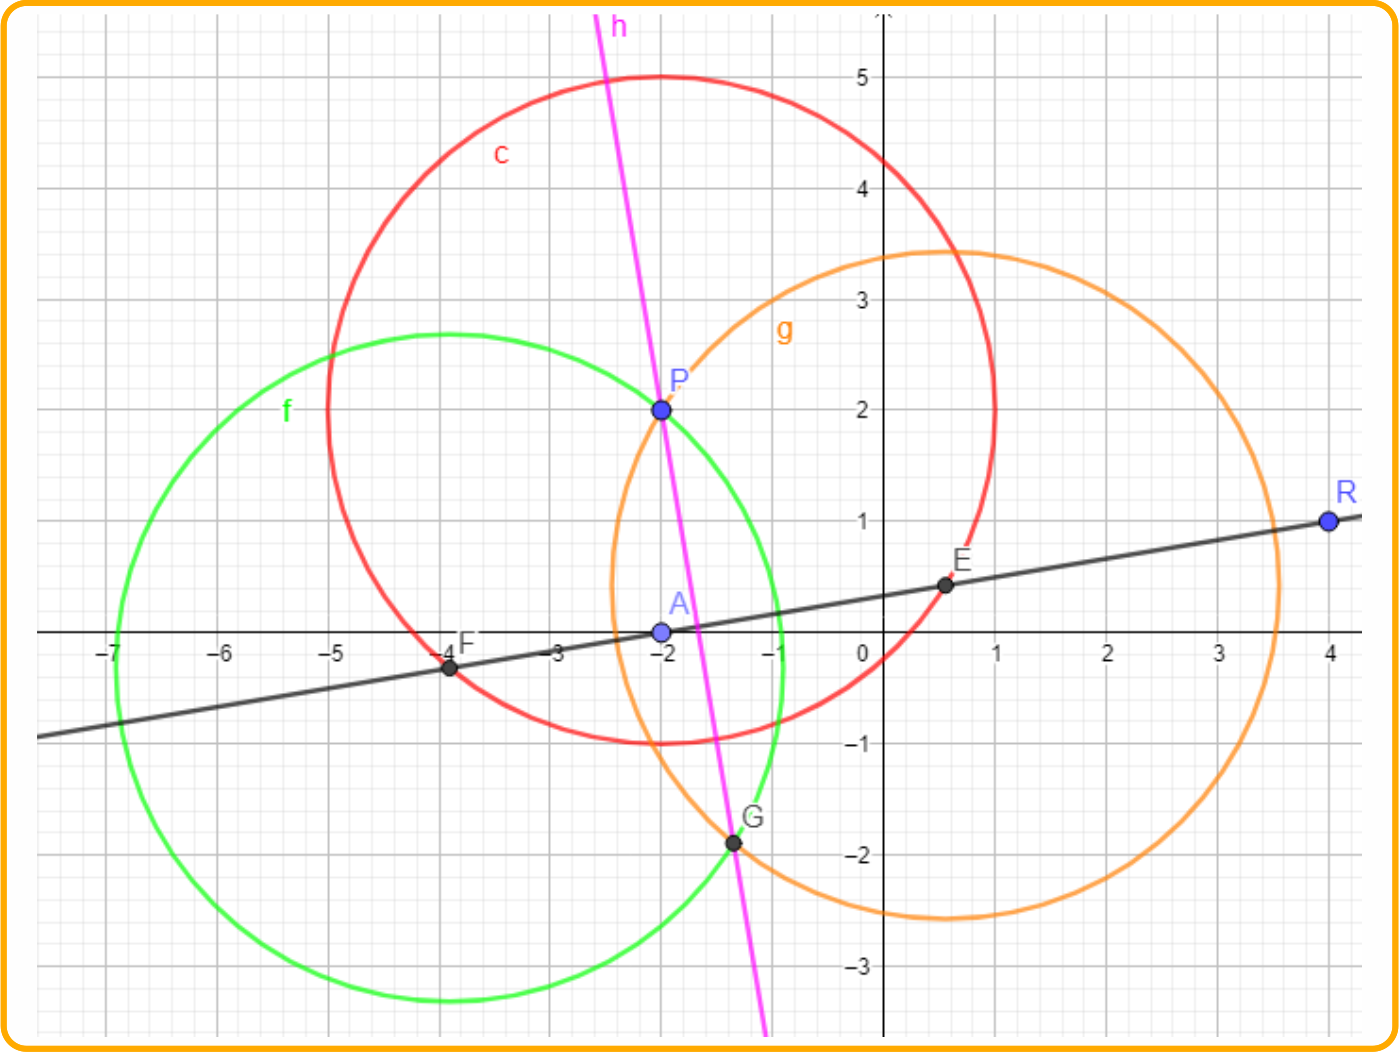
\includegraphics[height=8cm]{Figuras/T01_Atividade03_Fig05.png}
    \caption{Atividade III - Etapa \ref{Atividade03_Etapa13}}
    \label{Atividade03_Etapa13_Imagem}
\end{figure}

\item Selecione o ícone em destaque e clique na opção {\it ângulo}. \label{Atividade03_Etapa14}
\begin{figure}[H]
    \centering
    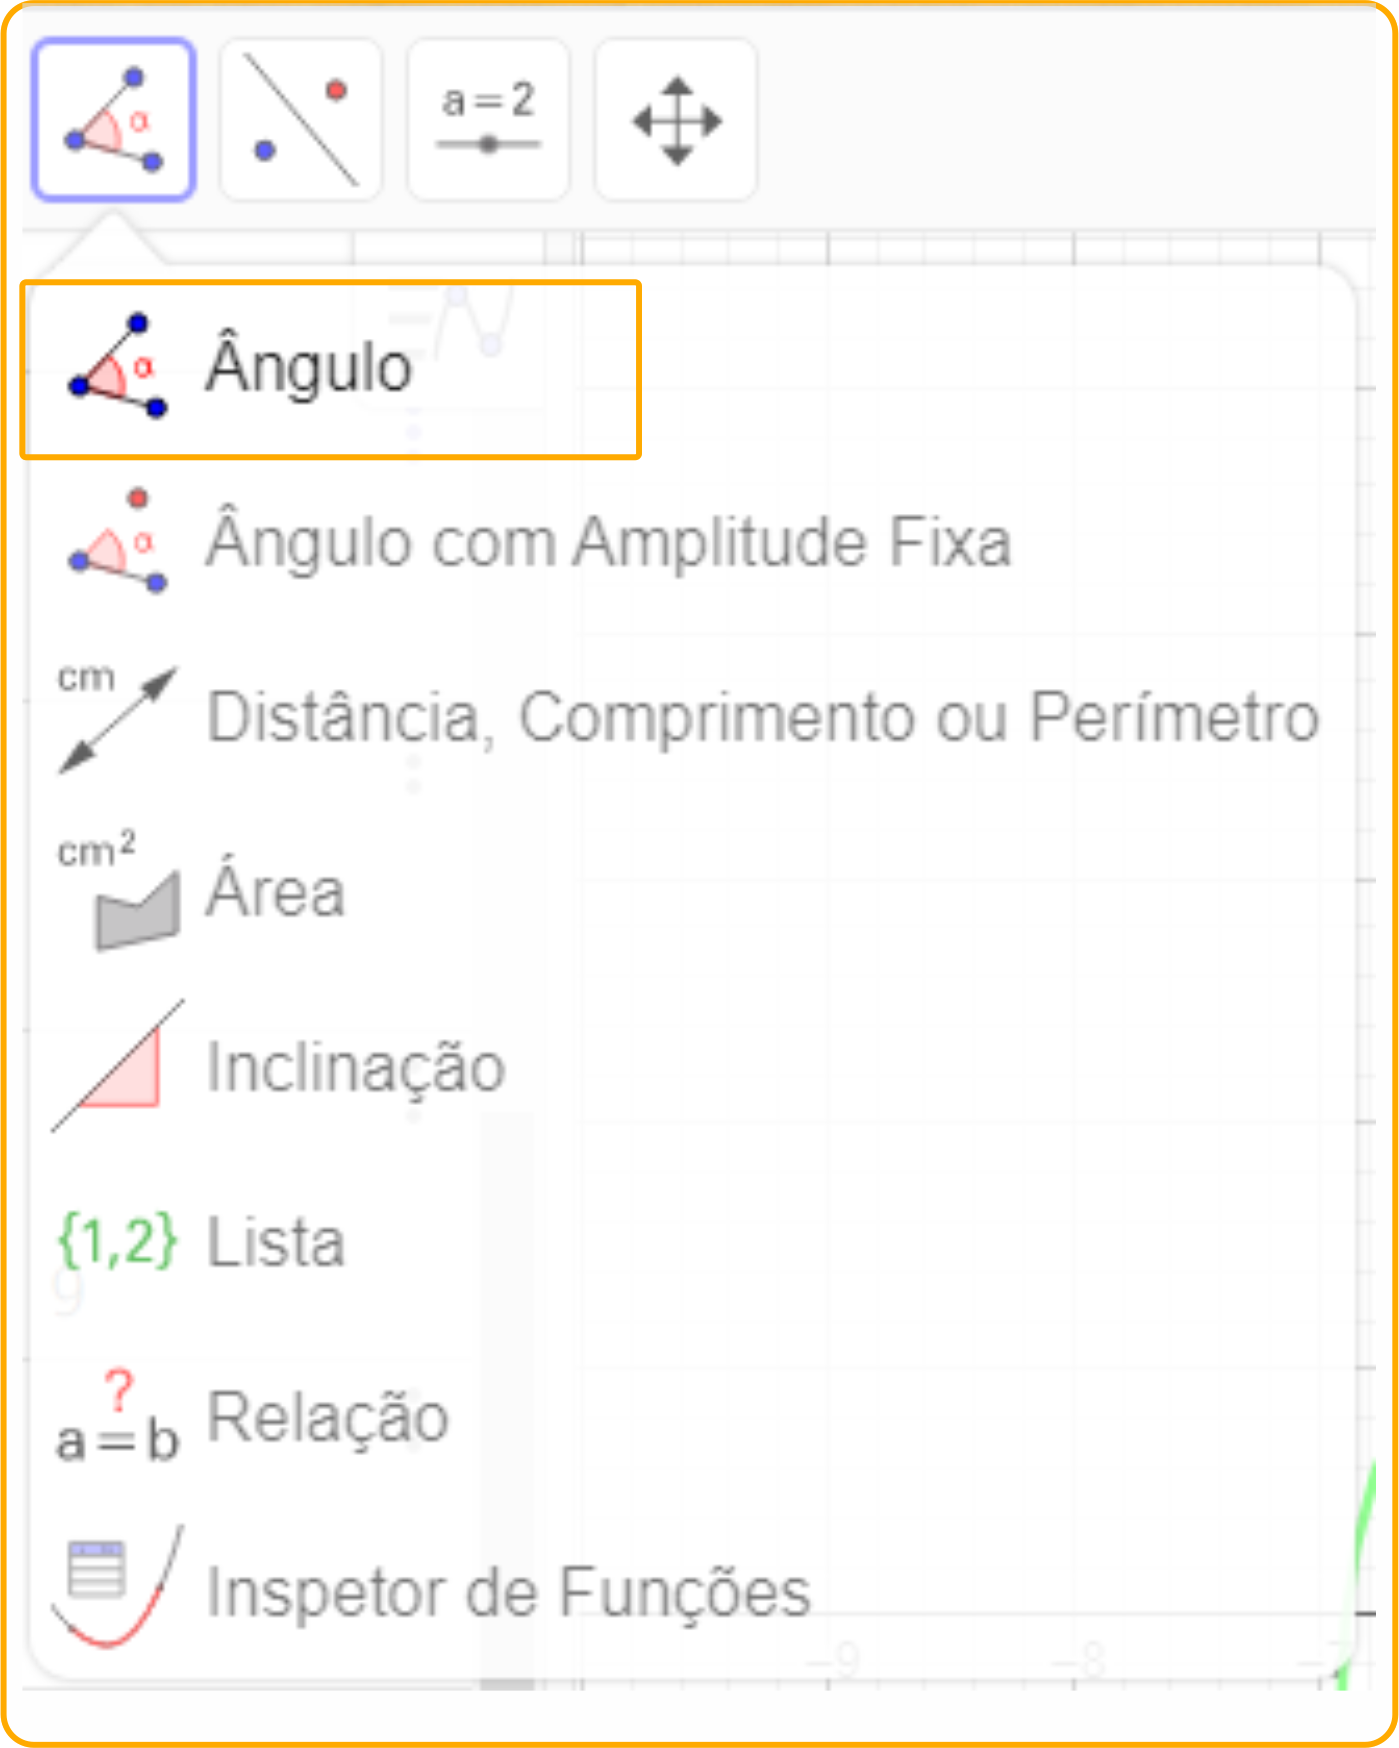
\includegraphics[height=8cm]{Figuras/T01_Elemento08.png}
    \caption{Atividade III - Etapa \ref{Atividade03_Etapa14}}
    \label{Atividade03_Etapa14_Imagem}
\end{figure}

\item Marque a interseção entre as retas $r$ e ${\color{magenta}{h}}$ para que o GeoGebra calcule o ângulo formado pelas retas. Note que o ângulo é de $90^\circ$! \label{Atividade03_Etapa15}
\begin{figure}[H]
    \centering
    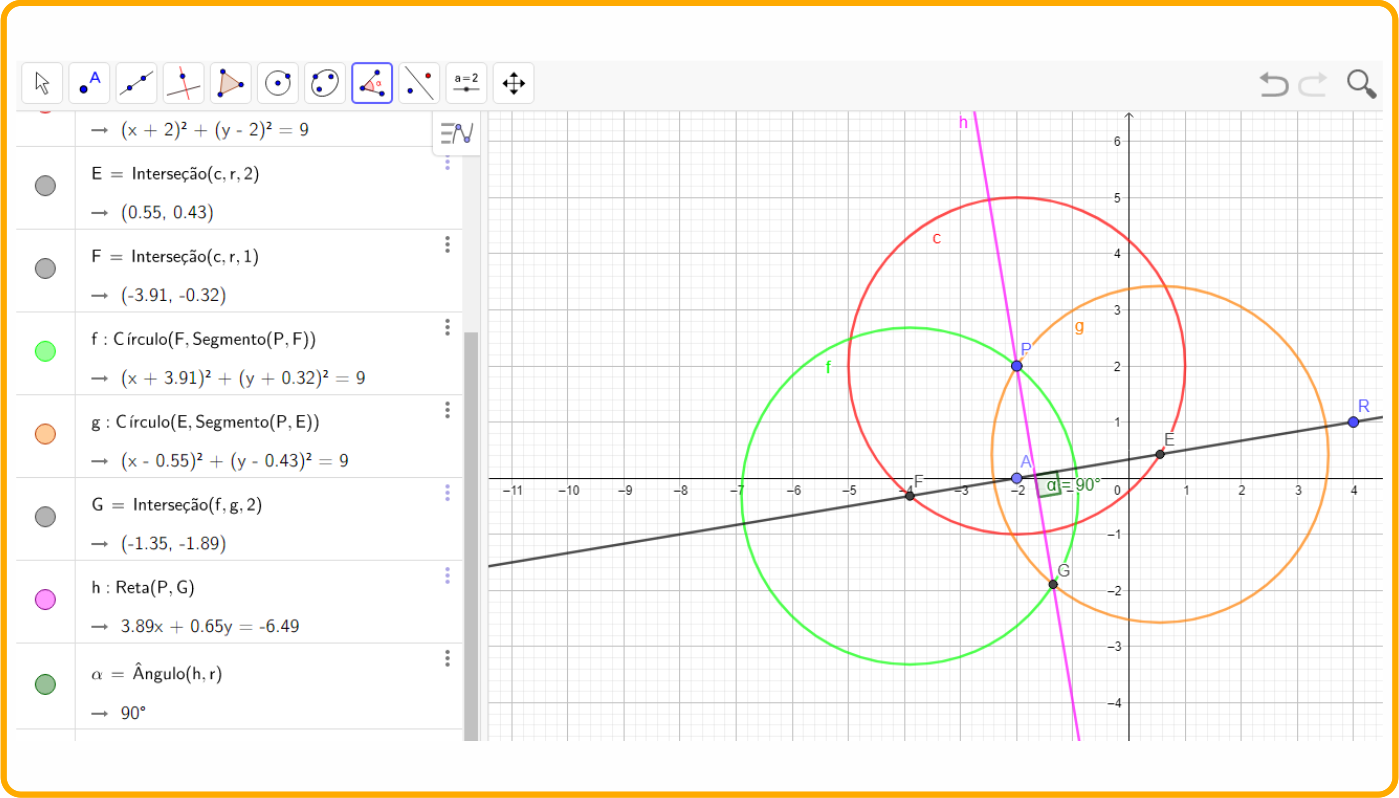
\includegraphics[height=7cm]{Figuras/T01_Atividade03_Fig06.png}
    \caption{Atividade III - Etapa \ref{Atividade03_Etapa15}}
    \label{Atividade03_Etapa15_Imagem}
\end{figure}

Isso ocorre pois como $\overline{PF}$ = $\overline{PE}$ e $\overline{GF}$ = $\overline{GE}$, então a reta $\overline{PG}$ é a mediatriz de $\overline{EF}$, e portanto, é perpendicular à $r$.
\end{enumerate}

\newpage 

%%%%%%% SEÇÃO 04 - VEJA A AULA PRONTA! %%%%%%%%
\section{Veja a aula!}
Você pode acessar o passo a passo desta aula com todas as atividades propostas clicando \bf{\href{https://www.geogebra.org/m/v5cyvu8t}{aqui}}.

\newpage
%%%%%%% SEÇÃO 05 - EXERCÍCIOS! %%%%%%%%
\section{Exercícios propostos}

Agora que você já aprendeu a usar o GeoGebra, que tal realizar alguns exercícios para praticar um pouco mais?

\begin{enumerate}[{Exercício} 1.]
\item Observe que os pontos $M$, $N$ e $O$ são pontos médios dos segmentos $\overline{AB}$, $\overline{BC}$ e $\overline{AC}$ respectivamente.
\begin{figure}[H]
    \centering
    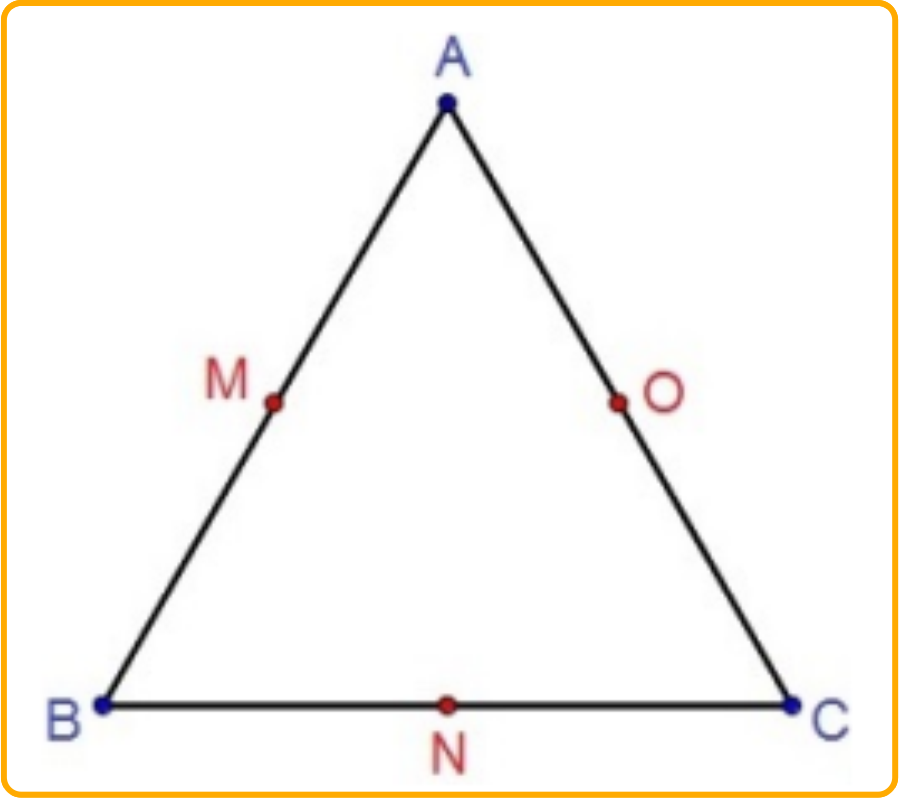
\includegraphics[height=7cm]{Figuras/T01_Exercicio01.png}
    \caption{Exercício 01}
\end{figure}
    \begin{enumerate}
        \item Desenhe uma circunferência com centro em $A$ passando por $M$.
        \item Desenhe outra circunferência com centro em $B$ passando por $N$.
        \item Desenhe uma terceira circunferência com centro em $C$ e passando por $O$.
    \end{enumerate}

\item Faça sete circunferências, cada uma com centro em cada um dos pontos dados abaixo, de modo que:
\begin{enumerate}
    \item A primeira tenha centro em $A$ e raio $\overline{AG}$.
    \item A segunda com centro em $B$ e raio $\overline{BG}$.
    \item A terceira com centro em $G$ e raio $\overline{GA}$.
    \item A quarta com centro em $F$ e raio $\overline{FG}$.
    \item A quinta com centro em $C$ e raio $\overline{CG}$.
    \item A sexta com centro em $E$ e raio $\overline{BG}$.
    \item A sétima com centro em $D$ e raio $\overline{DG}$.
\end{enumerate}
\begin{figure}[H]
    \centering
    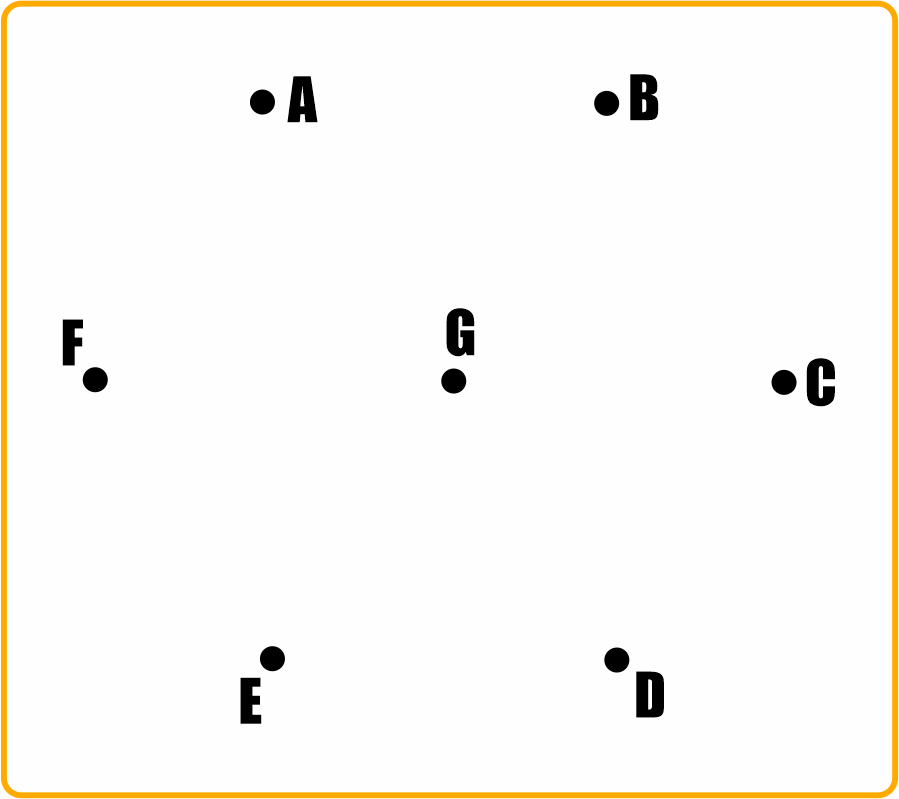
\includegraphics[height=7cm]{Figuras/T01_Exercicio02.png}
    \caption{Exercício 02}
\end{figure}

\item Dada uma reta $t$, construa duas circunferências $c$ e $d$, tal que $c$ seja tangente à circunferência $d$ e à reta $t$ no ponto $T$.

\end{enumerate}


\bibliography{referencias.bib}
\bibliographystyle{plain}
\end{document}
